% !TEX program = xelatex
\documentclass[UTF8,fontset=fandol,a4paper,11pt]{ctexart}
\usepackage[margin=21mm,top=23mm,bottom=22mm,headheight=16pt]{geometry}
\usepackage{amsmath,amssymb,mathtools,bm}
\usepackage{tikz}
\usetikzlibrary{arrows.meta,calc,angles,quotes,patterns}
\usepackage{xcolor,booktabs,array,longtable,enumitem,fancyhdr,needspace}
\usepackage[unicode,hidelinks]{hyperref}
\definecolor{ink}{HTML}{24343C}
\definecolor{accent}{HTML}{166A70}
\definecolor{muted}{HTML}{65747A}
\definecolor{rulegray}{HTML}{D4DDE0}
\definecolor{warm}{HTML}{966037}
\color{ink}
\setlength{\parindent}{2em}
\setlength{\parskip}{4pt}
\linespread{1.12}
\AtBeginDocument{\setlength{\abovedisplayskip}{6pt plus 2pt minus 1pt}
\setlength{\belowdisplayskip}{6pt plus 2pt minus 1pt}
\setlength{\abovedisplayshortskip}{0pt plus 1pt}
\setlength{\belowdisplayshortskip}{4pt plus 1pt}}
\setlist[enumerate]{label=(\arabic*),leftmargin=2.3em,itemsep=3pt,topsep=4pt}
\setlist[itemize]{leftmargin=2em,itemsep=2pt,topsep=4pt}
\allowdisplaybreaks[1]
\setlength{\emergencystretch}{2em}
\setcounter{secnumdepth}{0}
\providecommand{\tightlist}{\setlength{\itemsep}{0pt}\setlength{\parskip}{0pt}}
\ctexset{section={format=\Large\bfseries\color{accent},beforeskip=10pt,afterskip=9pt},
subsection={format=\normalsize\bfseries\color{accent},beforeskip=10pt,afterskip=4pt},
subsubsection={format=\normalsize\bfseries,beforeskip=8pt,afterskip=3pt}}
\pagestyle{fancy}
\fancyhf{}
\fancyhead[L]{\small\color{muted}物理学难题集萃}
% 页眉仅保留书名；版本名称只在封面显示。
\fancyfoot[L]{\small\color{muted}\chapterlabel}
\fancyfoot[R]{\small\thepage}
\renewcommand{\headrulewidth}{0.4pt}
\renewcommand{\footrulewidth}{0pt}
\newcommand{\dd}{\mathop{}\!\mathrm{d}}
\newcommand{\vect}[1]{\bm{#1}}
\newcommand{\tagline}[1]{\noindent{\small\color{muted}#1}\par}
\newcommand{\result}[1]{\begin{equation*}\boxed{#1}\end{equation*}}
\newcommand{\figcaption}[1]{\par\vspace{2pt}{\small\color{muted}#1}\par}
\newcommand{\teach}[2]{\Needspace{4\baselineskip}\subsection*{讲解要点与追问}#1\par\smallskip\noindent\textbf{追问：}#2\par}
\newcommand{\workarea}{\par\vspace{7mm}\noindent{\small\color{muted}作答区}\par\vspace{4mm}
\noindent\textcolor{rulegray}{\rule{\linewidth}{0.3pt}}\par\vspace{16mm}
\noindent\textcolor{rulegray}{\rule{\linewidth}{0.3pt}}\par\vspace{16mm}
\noindent\textcolor{rulegray}{\rule{\linewidth}{0.3pt}}\par\vspace{16mm}
\noindent\textcolor{rulegray}{\rule{\linewidth}{0.3pt}}}
\tikzset{axis/.style={-{Stealth[length=2mm]},thin,color=muted},
motion/.style={-{Stealth[length=2.3mm]},thick,color=accent},
force/.style={-{Stealth[length=2.3mm]},thick,color=warm},
traj/.style={thick,color=accent},guide/.style={dashed,thin,color=muted},
object/.style={thick,color=ink},every node/.style={font=\small}}\widowpenalty=10000\clubpenalty=10000\displaywidowpenalty=10000

\newcommand{\chapterlabel}{热学第二章\quad 热力学第一、第二定律}
\hypersetup{pdftitle={热学第二章 热力学第一、第二定律·学生解答版},pdfauthor={},pdfsubject={热学第二章第1--25题}}
\begin{document}
\pdfbookmark[0]{热学第二章 热力学第一、第二定律}{cover}
\thispagestyle{empty}\vspace*{20mm}
\noindent{\Huge\bfseries 物理学难题集萃}\par\vspace{8mm}
\noindent{\LARGE 热学第二章}\par\vspace{5mm}
\noindent{\LARGE 热力学第一、第二定律}\par\vspace{10mm}
\noindent{\Large\color{accent}学生解答版}\par\vspace{8mm}
\noindent\textcolor{accent}{\rule{\linewidth}{1pt}}\par\vspace{8mm}
\noindent 第1--25题\par\vspace{5mm}
\noindent 完整演算、图示分析与条件讨论。\par\vfill\clearpage
\pdfbookmark[1]{题目目录}{contents}\section*{题目目录}
\begin{longtable}{@{}>{\color{accent}\bfseries}r p{120mm}@{}}
\toprule 题号 & 题目\\\midrule
1 & 循环过程证明比热不可能恒定 \\
2 & 平移等温线确定过程比热曲线 \\
3 & 直线过程的温度图像与比热正负 \\
4 & 单原子双原子混合理想气体的绝热指数 \\
5 & 热功效率恒定过程中的总功 \\
6 & 变热容量过程的内能增量与作功 \\
7 & 钢丝棉氧化反应中的热量与内能变化 \\
8 & 双活塞气缸加热的分段末温 \\
9 & 绝热压缩后缓慢扩散的终温 \\
10 & 带阀绝热活塞与电热器的能量分配 \\
11 & 绝热左筒与等温右筒的活塞平衡 \\
12 & 带阀隔板气缸的分段绝热压缩功 \\
13 & 绝热容器中推活塞后混合的终压 \\
14 & 潮湿空气越山降雨的热力学估算 \\
15 & U形管水银振动与封闭空气绝热弹性 \\
16 & 由声速驻波判断碘蒸气分子类型 \\
17 & 两个三角循环效率的比较 \\
18 & 多条过程线构成循环的效率比较 \\
19 & 氦气三直线循环效率 \\
20 & 直线加绝热线循环的效率与极值温度 \\
21 & 圆形准静态循环的功、热量和转折点 \\
22 & 可逆卡诺空调的维持室温与最高外温 \\
23 & 绝热细棒热平衡过程的熵增 \\
24 & 氧气复合循环效率与 S-T 图像 \\
25 & 由 T-S 直线导出理想气体过程方程 \\\bottomrule\end{longtable}

\clearpage

\pdfbookmark[2]{第 1 题 循环过程证明比热不可能恒定}{q1}

\section*{第 1 题\quad 循环过程证明比热不可能恒定}

一定量理想气体经历图示顺时针准静态循环，$p-V$图中闭合曲线围成的面积不为零。以$\delta Q=M c\dd T$定义沿过程的质量比热，$M$为气体质量。证明该循环的过程比热$c$不可能处处为同一个有限常量，并讨论循环反向时的结论。

\begin{center}\begin{minipage}{0.96\linewidth}\centering
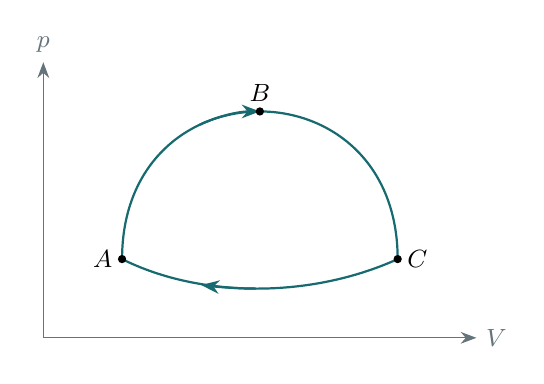
\begin{tikzpicture}[x=1cm,y=1cm,font=\small]
\draw[axis] (0,0)--(5.5,0) node[right] {$V$};
\draw[axis] (0,0)--(0,3.5) node[above] {$p$};
\draw[traj] (1,1) .. controls (1,3.5) and (4.5,3.5) .. (4.5,1)
 .. controls (3.4,.5) and (2,.5) .. (1,1);
\draw[motion] (1.986125,2.70625) .. controls (2.225,2.82) and (2.49,2.875) .. (2.75,2.875);
\draw[motion] (2.705,.625) .. controls (2.48,.625) and (2.23,.645) .. (2.006,.67);
\fill (1,1) circle(1.5pt) node[left] {$A$};
\fill (2.75,2.875) circle(1.5pt) node[above] {$B$};
\fill (4.5,1) circle(1.5pt) node[right] {$C$};
\end{tikzpicture}\figcaption{图 热2.1　闭合路径包围非零面积；箭头给出循环方向。}\end{minipage}\end{center}

\Needspace{8\baselineskip}\subsection*{解答}

\textbf{沿闭合路径列第一定律。}气体一周后回到同一状态，内能是状态函数，因此$\Delta U=0$。解图热2.1A沿$A\to B\to C\to A$运行，有向面积为正，气体对外功
\[W=\oint p\dd V>0.\]
取气体对外功为正，一周的\emph{净}吸热$Q=W>0$。这里各微元吸热取正、放热取负，求和得到净吸热。
\begin{center}\begin{minipage}{0.96\linewidth}\centering
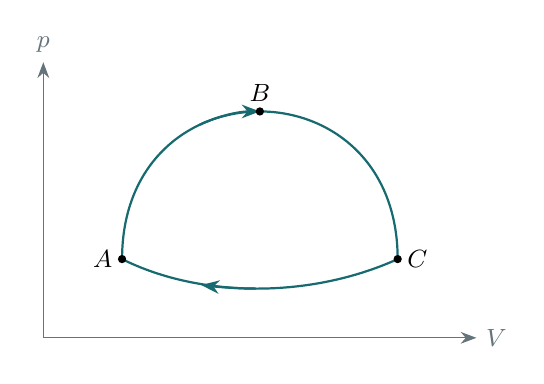
\begin{tikzpicture}[x=1cm,y=1cm,font=\small]
\draw[axis] (0,0)--(5.5,0) node[right] {$V$};
\draw[axis] (0,0)--(0,3.5) node[above] {$p$};
\draw[traj] (1,1) .. controls (1,3.5) and (4.5,3.5) .. (4.5,1)
 .. controls (3.4,.5) and (2,.5) .. (1,1);
\draw[motion] (1.986125,2.70625) .. controls (2.225,2.82) and (2.49,2.875) .. (2.75,2.875);
\draw[motion] (2.705,.625) .. controls (2.48,.625) and (2.23,.645) .. (2.006,.67);
\fill (1,1) circle(1.5pt) node[left] {$A$};
\fill (2.75,2.875) circle(1.5pt) node[above] {$B$};
\fill (4.5,1) circle(1.5pt) node[right] {$C$};
\end{tikzpicture}\figcaption{解图 热2.1A　循环面积给净功，闭合状态给内能增量；净热量由两者确定。}\end{minipage}\end{center}
反设每一微小过程的比热均为同一个有限常量$c$，则
\[\delta Q=Mc\dd T,\qquad Q=\oint\delta Q=Mc\oint\dd T.\]
温度也为状态量，闭合路径满足$\oint\dd T=0$，遂有$Q=0$，与$Q=W>0$矛盾。因此$c$不可能沿全循环保持同一有限值。

\textbf{反向循环与自交路径。}反向循环时$W<0$、$Q<0$，仍与反设的$Q=0$矛盾。若路径自交，只需总有向面积非零，即$W\ne0$，证明仍成立；面积相消为零时，整体积分给 $Q=W=0$，对非零面积的闭合子回路可分别使用同一论证。温度瞬时不变而热量微元不为零处，比热还可能无定义或发散。论证所用的状态函数、固定系统和第一定律也适用于具有这些条件的其他热力学系统。
\subsubsection*{把每一微元与闭路积分对应起来}
把解图热2.1A的循环依次分成足够短的过程段，以$T_i$表示分点温度。
各段温度变化满足
\[
\sum_i(T_{i+1}-T_i)=T_{\rm f}-T_{\rm i}=0.
\]
温差逐项相消，只使用了初、末状态相同。实际热量应为
$Q_{\rm net}=\sum_i\delta Q_i$；只有在反设$c_i=c_0$处处为同一有限值后，才能写成
\[
Q_{\rm net}=\lim\sum_i Mc_i(T_{i+1}-T_i)
=Mc_0(T_{\rm f}-T_{\rm i})=0.
\]
一般过程中各段的 $c_i$ 随状态及路径变化，热量相加时各自与对应温差相乘。
顺时针非零面积$\mathcal A$给$Q_{\rm net}=W_{\rm cyc}=\mathcal A>0$，
反向则给$-\mathcal A$；两种方向都与恒定有限比热的积分结果矛盾。

还可从局部第一定律看出图中各点的过程比热怎样产生。
对准静态理想气体，$c_V$按单位质量计，有
\[
\delta Q=Mc_V\dd T+p\dd V,\qquad
c=c_V+\frac pM\frac{\dd V}{\dd T}\quad(\dd T\ne0).
\]
同一种气体的$c_V$可以是常量，沿路径的$c$仍因$\dd V/\dd T$变化。
等温段若有$p\dd V\ne0$，则$\dd T=0$而$\delta Q\ne0$，此处无法定义有限$c$；
绝热且$\dd T\ne0$的段则有$c=0$。

\begin{center}\begin{minipage}{0.96\linewidth}\centering
\begin{tikzpicture}[x=1cm,y=1cm]
\draw[axis] (0,0)--(6,0) node[right] {$V$};
\draw[axis] (0,0)--(0,3.7) node[above] {$p$};
\coordinate (C) at (3,2);
\draw[traj] (C)--(1,3)--(1,1)--cycle;
\draw[traj] (C)--(5,3)--(5,1)--cycle;
\draw[motion] (1,2.6)--(1,1.7);
\draw[motion] (5,2.6)--(5,1.7);
\fill (C) circle(1.7pt) node[above] {$C$};
\node at (1.7,2) {$W_L<0$};
\node at (4.3,2) {$W_R>0$};
\node[below,align=center] at (3,.65) {两瓣面积相等，$W_L+W_R=0$};
\end{tikzpicture}
\figcaption{解图 热2.1B　同一交点$C$把自交路径分成两个非零净功的闭合子回路。}
\end{minipage}\end{center}
解图热2.1B的两个叶瓣各自围成非零面积，分别对应净功非零的闭合过程。
对全路径积分得到$0=0$时，前面的整体反证没有矛盾；
但左瓣从$C$出发又回到$C$，本身已满足$\Delta U_L=\Delta T_L=0$、
$Q_L=W_L\ne0$。单独对左瓣使用同一反证，便能排除全路径处处同一有限$c$。
整体积分由两瓣的有向面积相消给出 $0=0$，单瓣积分则分别给出非零净热量，提供了更细的路径信息。
相反，等压线上往返的每一闭合段都没有净面积，理想气体可始终取$c=c_p$。
推广到其他物质时，所需条件仍是明确的温度、内能状态和第一定律；
每次积分均跟随同一固定质量和组成的系统，初、末状态由该系统的一组状态量确定。


\Needspace{18\baselineskip}

\pdfbookmark[2]{第 2 题 平移等温线确定过程比热曲线}{q2}

\section*{第 2 题\quad 平移等温线确定过程比热曲线}

质量为$M$、摩尔质量为$\mu$的理想气体，定容比热$c_V$为常量。其准静态过程$x$在$p-V$平面上向下平移$p_0>0$后，恰成为温度$T_0$的等温线。求过程$x$的温度下限及其在曲线上的位置；导出$c$与$p$的关系，画出$c-p$曲线。

\begin{center}\begin{minipage}{0.96\linewidth}\centering
\begin{tikzpicture}[x=1cm,y=1cm,font=\small]\draw[axis] (0,0)--(5.5,0) node[right] {$V$};\draw[axis] (0,0)--(0,3.5) node[above] {$p$};
\draw[traj,domain=.65:5,samples=60] plot (\x,{1+1.6/\x});\draw[guide,domain=.65:5,samples=60] plot (\x,{1.6/\x});\draw[<->] (3,.533)--(3,1.533) node[right,midway]{$p_0$};\node[right] at (4.7,1.5) {$x$};\node[right] at (3.7,.25) {$T=T_0$};
\end{tikzpicture}\figcaption{图 热2.2　实线向下平移$p_0$成为等温虚线，同一体积处比较压强。}\end{minipage}\end{center}

\Needspace{8\baselineskip}\subsection*{解答}

\textbf{由同体积两点写方程。}设$\nu=M/\mu$。解图热2.2A中同一体积V上的两点压差为$p_0$，较低点在$T_0$等温线上：
\[(p-p_0)V=\nu RT_0,\qquad pV=\nu RT.\]
两式相减，或消去V，分别得到
\[T=T_0+\frac{p_0V}{\nu R},\qquad
V=\frac{\nu R}{p_0}(T-T_0),\qquad p=\frac{p_0T}{T-T_0}.\]
\begin{center}\begin{minipage}{0.96\linewidth}\centering
\begin{tikzpicture}[x=1cm,y=1cm,font=\small]
\draw[axis] (0,0)--(5.5,0) node[right] {$V$};
\draw[axis] (0,0)--(0,3.8) node[above] {$p$};
\draw[traj,domain=.65:5,samples=70] plot (\x,{1+1.6/\x});
\draw[guide,domain=.65:5,samples=70] plot (\x,{1.6/\x});
\draw[guide] (0,1) node[left] {$p_0$}--(5.1,1);
\node[below] at (4.1,.39) {$T_0$等温线};
\draw[guide] (2,0) node[below] {$V$}--(2,1.8);
\fill (2,.8) circle(1.5pt) node[below left] {$P_0$};
\fill (2,1.8) circle(1.5pt) node[above left] {$P$};
\draw[<->] (2.18,.8)--(2.18,1.8) node[midway,right] {$p_0$};
\fill (1,2.6) circle(1.5pt) node[above right] {$A$};
\fill (4,1.4) circle(1.5pt) node[above right] {$B$};
\draw[motion] (2.9,{1+1.6/2.9})--(3.4,{1+1.6/3.4});
\node[align=center] at (3.6,3.1) {$T=T_0+p_0V/(\nu R)$\\$V\to0^+:T\to T_0^+$};
\end{tikzpicture}\figcaption{解图 热2.2A\quad 同一$V$处，实线状态与$T_0$等温线状态的压强差为$p_0$；有限体积时$T>T_0$。}\end{minipage}\end{center}
物理区域为$V>0$、$p>p_0$，故$T>T_0$。随V增加，T单调增加；整条曲线的温度下限为$T_0$，只在左上方$V\to0^+$、$p\to\infty$时趋近，该端点为不取到的极限。若只取图上的有限曲线段，最低温度在其左上端，且大于$T_0$。

\textbf{由温度微元求比热。}这里$c_V,c$按单位质量计，故
\[\dd V=\frac{MR}{\mu p_0}\dd T,\qquad
\delta Q=Mc_V\dd T+p\dd V
=M\left(c_V+\frac{Rp}{\mu p_0}\right)\dd T.\]
可把所得热容量看成两项的和：单位质量升温$\dd T$使内能增加$c_V\dd T$，同时沿图热2.2A的平移曲线膨胀，对外功为
\[\frac{p\dd V}{M}=\frac{Rp}{\mu p_0}\dd T.\]
这条路径的单位质量体积变化率为 $R/(\mu p_0)$，相应作功项随当前压强 $p$ 增加。当$p$很大时，同样的温升仍对应相同的体积增量，却要克服更大的压强，所需热量便更多。

于是
\result{c(p)=c_V+\frac{R}{\mu p_0}p,\qquad p>p_0.}
\begin{center}\begin{minipage}{0.96\linewidth}\centering
\begin{tikzpicture}[x=1cm,y=1cm,font=\small]\draw[axis] (0,0)--(5.5,0) node[right] {$p$};\draw[axis] (0,0)--(0,3.5) node[above] {$c$};
\draw[traj] (1,1.3)--(4.8,3.2);\draw[guide] (1,0) node[below]{$p_0$}--(1,1.3)--(0,1.3) node[left]{$c_p$};\draw[ink,fill=white] (1,1.3) circle(2pt);\node[align=left] at (3.45,.75) {$p>p_0$\\斜率 $R/(\mu p_0)$};
\end{tikzpicture}\figcaption{解图 热2.2B　只取$p>p_0$的直线部分；端点$c_p$不属于有限体积过程。}\end{minipage}\end{center}
解图热2.2B的$c-p$图为斜率$R/(\mu p_0)$的直线，其实际定义域只取$p>p_0$。当$p\to p_0^+$时$c\to c_V+R/\mu=c_p$；这对应$V\to\infty,T\to\infty$。沿V增大的方向，温度上升、气体作正功且吸热，$c>c_p>0$，与公式相符。
\subsubsection*{两种温度表示及有限过程的热量}
解图热2.2A的竖线连接相同体积的两个状态，设上端为$P$、下端为$P_0$。
$P_0$在$T_0$等温线上，故$(p-p_0)V=\nu RT_0$；
上端$P$的温度为$T$，有$pV=\nu RT$。分别作差和取比，给出
\[
p_0V=\nu R(T-T_0),\qquad
\frac T{T_0}=\frac p{p-p_0}.
\]
因此当$V$由小变大时，$T$按直线规律升高，$p$却沿双曲线下降。
每一条温度高于$T_0$的等温线与过程$x$只交于一个状态；
对应的体积$V=\nu R(T-T_0)/p_0$随温度增加。
若实际过程从有限的$V_a$开始，其最低温度为$T_a$；
只有把整条正体积曲线都作为定义域时，才以$T_0$为不取到的下确界。

将比热写成温度的函数，再分别取低温和高温极限。
由$p/p_0=T/(T-T_0)$，有
\[
c(T)=c_V+\frac R\mu\frac T{T-T_0}
=c_p+\frac{RT_0}{\mu(T-T_0)},\qquad T>T_0.
\]
求导得到
\[
\frac{\dd c}{\dd T}=-\frac{RT_0}{\mu(T-T_0)^2}<0,\qquad
\frac{\dd c}{\dd V}=-\frac{\nu R^2T_0}{\mu p_0V^2}<0.
\]
所以$c$随$p$增加而增加，随$V$和$T$增加却减小。
解图热2.2B的左端$c_p$对应很大的体积和温度；左上方的低温极限反而有$c\to+\infty$。
在图中标出两个状态$A,B$，令$0<V_a<V_b$，则
$p_a>p_b>p_0$、$T_b>T_a>T_0$、$c_a>c_b>c_p$。

有限膨胀段的比热随温度变化，将 $c(T)$ 沿全段积分求热量。先由体积功求得
\[
\begin{aligned}
W_{a\to b}
&=\int_{V_a}^{V_b}\left(p_0+\frac{\nu RT_0}{V}\right)\dd V\\
&=p_0(V_b-V_a)+\nu RT_0\ln\frac{V_b}{V_a}\\
&=\nu R(T_b-T_a)+\nu RT_0
 \ln\frac{T_b-T_0}{T_a-T_0},\\
\Delta U&=Mc_V(T_b-T_a),\\
Q_{a\to b}&=Mc_p(T_b-T_a)+\nu RT_0
 \ln\frac{T_b-T_0}{T_a-T_0}.
\end{aligned}
\]
也可直接由$M\int_{T_a}^{T_b}c(T)\dd T$得到最后一式。
前一算法用图中$A\to B$曲线下的功面积，后一算法用$c(T)$积分，两者给同一热量。
对膨胀段，上述对数和温差均为正，所以吸热且作正功；反向压缩时二者同时反号，
但局部$c=\delta Q/(M\dd T)$仍为同一正值函数。
例如取$V_b=2V_a$且$V_a=\nu RT_0/p_0$，
则$T_a=2T_0,T_b=3T_0,p_a=2p_0,p_b=3p_0/2$，
\[
W=\nu RT_0(1+\ln2),\qquad
Q=Mc_pT_0+\nu RT_0\ln2.
\]
两端的局部比热分别为 $c_a=c_V+2R/\mu$ 与 $c_b=c_V+3R/(2\mu)$。全段平均比热为 $Q/[M(T_b-T_a)]$，由上式中的对数项确定。
比热的单位是$\mathrm{J/(kg\cdot K)}$，$R/\mu$与$c_V$同量纲；
对数的自变量 $V_b/V_a$ 为同种量的比值，量纲约去。


\Needspace{18\baselineskip}

\pdfbookmark[2]{第 3 题 直线过程的温度图像与比热正负}{q3}

\section*{第 3 题\quad 直线过程的温度图像与比热正负}

质量为$M$、摩尔质量为$\mu$的理想气体，定容比热$c_V=3R/(2\mu)$。气体沿直线由$A(V_0,2p_0)$到$B(2V_0,p_0)$。求$T(V)$并作图；求过程比热$c(V)$并作图，结合$\delta Q/(M\dd T)$解释各段$c$的正负。

\begin{center}\begin{minipage}{0.96\linewidth}\centering
\begin{tikzpicture}[x=1cm,y=1cm,font=\small]\draw[axis] (0,0)--(5.5,0) node[right] {$V/V_0$};\draw[axis] (0,0)--(0,3.5) node[above] {$p/p_0$};
\draw[traj] (1,2)--(2,1);\draw[motion] (1.25,1.75)--(1.65,1.35);\fill[ink] (1,2) circle(1.4pt);\node[above right] at (1,2) {A};
\fill[ink] (2,1) circle(1.4pt);\node[above right] at (2,1) {B};
\draw[guide] (1,0) node[below]{1}--(1,2)--(0,2) node[left]{2};\draw[guide] (2,0) node[below]{2}--(2,1)--(0,1) node[left]{1};
\end{tikzpicture}\figcaption{图 热2.3　直线连接两端状态；坐标按$V_0,p_0$归一化。}\end{minipage}\end{center}

\Needspace{8\baselineskip}\subsection*{解答}

\textbf{温度曲线。}由题图两端点，令$x=V/V_0$，$T_*=\mu p_0V_0/(MR)$，则
\[p=p_0(3-x),\qquad T=T_*x(3-x),\qquad 1\le x\le2.\]
这是开口向下的抛物线。$\dd T/\dd x=T_*(3-2x)$，故
\[T_{\max}=\frac94T_*\quad(x=3/2),\qquad T_A=T_B=T_{\min}=2T_*.\]
\begin{center}\begin{minipage}{0.96\linewidth}\centering
\begin{tikzpicture}[x=2.8cm,y=1cm]
\draw[axis] (.8,0)--(2.3,0) node[right] {$x=V/V_0$};
\draw[axis] (.8,0)--(.8,3.1) node[above] {$T/T_*$};
\draw[traj,domain=1:2,samples=70] plot (\x,{\x*(3-\x)});
\draw[guide] (1.5,0) node[below] {$3/2$}--(1.5,2.25)--(.8,2.25) node[left] {$9/4$};
\draw[guide] (.8,2) node[left] {$2$}--(2,2);
\fill (1,2) circle(1.5pt) node[above left] {$A$};
\fill (2,2) circle(1.5pt) node[above right] {$B$};
\draw (1,.04)--(1,-.04) node[below] {$1$};
\draw (2,.04)--(2,-.04) node[below] {$2$};
\fill[accent] (1.5,2.25) circle(1.5pt) node[above] {$T_{\max}$};
\end{tikzpicture}\figcaption{解图 热2.3A\quad 纵轴按温度尺度$T_*=\mu p_0V_0/(MR)$归一化；$x=3/2$处温度最高。}\end{minipage}\end{center}
\textbf{热量微元与转折。}气体沿A到B膨胀，$\dd V>0$。从状态方程和内能式分别有
\[M c_V\dd T=\frac32p_0(3-2x)\dd V,\qquad
p\dd V=p_0(3-x)\dd V.\]
相加得
\[\delta Q=p_0\left(\frac{15}{2}-4x\right)\dd V.\]
题图热2.3上某点的压强决定单位体积增量的功，温度曲线的斜率决定单位体积增量的内能变化。具体写成
\[\frac{\dd U}{\dd V}=\frac32p_0(3-2x),\qquad
\frac{\delta W}{\dd V}=p_0(3-x).\]
从$x=3/2$到$x=15/8$，第一项已为负，第二项仍为正且绝对值更大，因此$\delta Q=\dd U+\delta W>0$。这段过程中内能随温度下降，膨胀功大于吸热量，内能的减少补足两者之差。

因此吸放热转折在$x=15/8$，而温度极大在$x=3/2$，两点不同。用比热定义相除：
\result{c=\frac{R}{\mu}\frac{15-8x}{2(3-2x)}.}
\begin{center}\begin{minipage}{0.96\linewidth}\centering
\begin{tikzpicture}[x=5cm,y=.38cm]
\draw[axis] (.88,0)--(2.18,0) node[right] {$x=V/V_0$};
\draw[axis] (.88,-8)--(.88,9) node[above] {$c/(R/\mu)$};
\node[left] at (.88,0) {$0$};
\draw[guide] (1.5,-8)--(1.5,8.7) node[above] {$3/2$};
\draw[traj,domain=1:1.37,samples=75] plot (\x,{(15-8*\x)/(2*(3-2*\x))});
\draw[traj,domain=1.59:2,samples=90] plot (\x,{(15-8*\x)/(2*(3-2*\x))});
\draw[motion] (1.35,7)--(1.37,7.77);
\draw[motion] (1.62,-4.25)--(1.59,-6.333333);
\fill (1,3.5) circle(1.4pt) node[above left] {$A$};
\fill (2,.5) circle(1.4pt) node[above right] {$B$};
\draw (1,.12)--(1,-.12) node[below] {$1$};
\draw (2,.12)--(2,-.12) node[below] {$2$};
\fill[accent] (1.875,0) circle(1.5pt);
\draw[guide] (1.875,0)--(1.875,-1.6) node[below] {$15/8$};
\node at (1.12,6.4) {$c>0$};
\node at (1.72,-4.5) {$c<0$};
\node at (2.04,3.5) {$c>0$};
\end{tikzpicture}\figcaption{解图 热2.3B　横向实轴为$c=0$，两支在$x=3/2$处不连接；箭头指向被截去的发散部分。}\end{minipage}\end{center}
沿解图热2.3B的两条分支，将温差和热量的符号分别列为
\begin{center}\begin{tabular}{cccc}\toprule
体积区间 & $\dd T$ & $\delta Q$ & $c$\\\midrule
$1<x<3/2$ & $+$ & $+$ & $+$\\
$3/2<x<15/8$ & $-$ & $+$ & $-$\\
$15/8<x<2$ & $-$ & $-$ & $+$\\\bottomrule\end{tabular}\end{center}
在$x\to(3/2)^-$时$c\to+\infty$，从右侧趋近时$c\to-\infty$；极大温度点$\dd T=0$而热量一阶不为零，比热无有限值。在 $x=15/8$ 处 $c=0$，热量微元过零，该点左侧吸热、右侧放热。当地绝热线与直线过程相切。负比热段中气体吸热却降温，是因为对外作功超过吸热量，内能仍减少。在两端代入各自的体积，得 $c_A=7R/(2\mu)$、$c_B=R/(2\mu)$。
\subsubsection*{直线过程中的温度极大点与热量零点}
题图热2.3中，压强随体积线性变化，温度则由沿途各状态的压强与体积之积决定。
直线斜率为$(p_B-p_A)/(V_B-V_A)=-p_0/V_0$，因此
\[
p=2p_0-\frac{p_0}{V_0}(V-V_0)=3p_0-\frac{p_0}{V_0}V.
\]
代入$pV=(M/\mu)RT$，展开为
\[
T=-\frac{\mu p_0}{MRV_0}V^2+\frac{3\mu p_0}{MR}V.
\]
这与前面的$T_*x(3-x)$完全相同，并给出
\[
\dd T=\frac{\mu p_0}{MR}(3-2x)\dd V.
\]
解图热2.3A的抛物线关于$x=3/2$对称，所以两个端点虽温度相等，
中间仍先升温后降温，形成图中的抛物线温度曲线。

在负比热区间，内能变化和膨胀功分别进入热力学第一定律。
取$x=7/4$、$\dd V>0$，有
\[
\dd U=-\frac34p_0\dd V,\qquad
\delta W=\frac54p_0\dd V,\qquad
\delta Q=\frac12p_0\dd V>0.
\]
气体吸入的热量不足以补偿对外作功，故仍降温。
在温度顶点$x=3/2$，$\dd T=0$，但
$\delta Q=(3/2)p_0\dd V$不为零，过程比热无有限值。
在$x_D=15/8$，则
\[
p_D=\frac98p_0,\qquad
\dd U=-\frac98p_0\dd V,\qquad
\delta W=\frac98p_0\dd V,\qquad\delta Q=0.
\]
此点的温度仍在下降，比热恰为零；两种特殊点由不同的微分量决定。

若另画经过$D$的单原子气体可逆绝热线，其局部斜率为
\[
\left.\frac{\dd p}{\dd V}\right|_{\rm ad,D}
=-\gamma\frac{p_D}{V_D}
=-\frac53\frac{(9/8)p_0}{(15/8)V_0}
=-\frac{p_0}{V_0}.
\]
它与题给直线在$D$相切。绝热线在邻近状态满足$pV^{5/3}=\mathrm{const}$，题给过程满足直线关系；两条曲线在$D$处有相同斜率，曲率则不同。

\subsubsection*{各子段的吸热、放热与全程能量变化}
由$\dd V=V_0\dd x$，任意子段的热量为
\[
Q_{a\to b}=p_0V_0
 \left[\frac{15}{2}x-2x^2\right]_{x_a}^{x_b}.
\]
正吸热累计到$D$，放热只发生在$D$之后，故
\[
Q_{\rm in}=\frac{49}{32}p_0V_0,\qquad
Q_{\rm out}=\frac1{32}p_0V_0,\qquad
Q_{\rm net}=\frac32p_0V_0.
\]
这里$Q_{\rm out}$表示放热量的正的绝对值。
另一方面，直线下方梯形面积给
\[
W_{A\to B}=\frac{p_A+p_B}{2}(V_B-V_A)=\frac32p_0V_0,
\]
初、末温度相同给$\Delta U=0$，所以$Q_{\rm net}=W$，与微元积分一致。
末段放热的$1/32$已计入积分，故净热量小于累计吸热量。
比热图上$3/2$处两支分开，$15/8$处平滑穿过零线，端点分别为$7R/(2\mu)$与$R/(2\mu)$；
温度转折、热量变号和两段有限热量因而在图上分别对应不同的位置与面积。


\Needspace{18\baselineskip}

\pdfbookmark[2]{第 4 题 单原子双原子混合理想气体的绝热指数}{q4}

\section*{第 4 题\quad 单原子双原子混合理想气体的绝热指数}

由$\nu_1$ mol单原子气体和$\nu_2$ mol双原子气体组成的理想混合气体，在常温下的准静态绝热方程为$pV^{11/7}=\text{常量}$。忽略双原子分子的振动自由度，求摩尔数比$\alpha=\nu_1/\nu_2$。

\begin{center}\begin{minipage}{0.96\linewidth}\centering
\begin{tikzpicture}[x=1cm,y=1cm,font=\small]\draw[object,fill=accent!6] (0,0) rectangle (6,1.8);\draw[guide] (3,0)--(3,1.8);\node[align=center] at (1.5,.9) {$\nu_1$ mol\\单原子};\node[align=center] at (4.5,.9) {$\nu_2$ mol\\双原子};\node[above] at (3,2.1){两组分混合，温度共同为$T$};
\end{tikzpicture}\figcaption{图 热2.4　图中虚线区分两组分的名称；两种分子均分布在总容积中。}\end{minipage}\end{center}

\Needspace{8\baselineskip}\subsection*{解答}

\textbf{两组分内能与热容量。}总摩尔数$\nu=\nu_1+\nu_2$；常温下单、双原子定容摩尔热容量分别为$3R/2$、$5R/2$。解图热2.4A中两份内能相加：
\[U=\frac32\nu_1RT+\frac52\nu_2RT=\nu C_VT,\qquad
C_V=\frac{(3\nu_1+5\nu_2)R}{2(\nu_1+\nu_2)}.\]
\begin{center}\begin{minipage}{0.96\linewidth}\centering
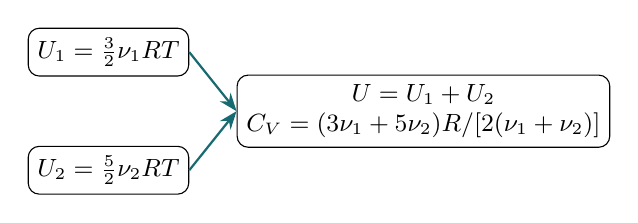
\begin{tikzpicture}[x=1cm,y=1cm,font=\small]\node[draw,rounded corners,align=center] (a) at (0,1.5){$U_1=\frac32\nu_1RT$};\node[draw,rounded corners,align=center] (b) at (0,0){$U_2=\frac52\nu_2RT$};\node[draw,rounded corners,align=center] (c) at (4,.75){$U=U_1+U_2$\\$C_V=(3\nu_1+5\nu_2)R/[2(\nu_1+\nu_2)]$};\draw[motion] (a.east)--(c.west);\draw[motion] (b.east)--(c.west);
\end{tikzpicture}\figcaption{解图 热2.4A　先把两组分总内能相加，再除以总摩尔数求混合气体摩尔热容量。}\end{minipage}\end{center}
定压过程由$p\dd V=\nu R\dd T$与第一定律得到
\[\delta Q=\nu C_V\dd T+p\dd V=\nu(C_V+R)\dd T,\qquad C_p=C_V+R.\]
\textbf{混合气体的绝热方程。}准静态绝热时$\nu C_V\dd T+p\dd V=0$。微分$pV=\nu RT$，消去$\dd T$：
\[(C_V+R)p\dd V+C_VV\dd p=0.\]
除以$C_VpV$，在组分和热容量不变时积分，得
\[\frac{\dd p}{p}+\gamma\frac{\dd V}{V}=0,\qquad
pV^\gamma=\text{常量},\quad\gamma=\frac{C_p}{C_V}.\]
将$\alpha=\nu_1/\nu_2$代入热容量，可直接写出组成与指数的关系：
\[\gamma=1+\frac R{C_V}
=\frac{5\alpha+7}{3\alpha+5}.\]
若$\alpha=0$，只有双原子气体，得$7/5$；若$\alpha\to\infty$，得$5/3$。题给$11/7$位于二者之间，故应有正的有限组成比。解图热2.4A中，各份内能相加得到总热容量，再求两个总热容量之比。这使 $\gamma$ 的组成权重由 $C_V$ 和 $C_p$ 共同决定。

由$\gamma=11/7$反求$C_V=R/(\gamma-1)=7R/4$，再与加权式联立：
\[\frac74=\frac{3\alpha+5}{2(\alpha+1)},\qquad
7(\alpha+1)=2(3\alpha+5).\]
\result{\alpha=3.}
取3 mol单原子与1 mol双原子，$C_V=(9/2+5/2)R/4=7R/4$，$C_p=11R/4$，指数确为11/7。加权依据是摩尔数；若振动自由度激发，$5R/2$不再适用，指数也可能随温度变化。
\subsubsection*{从总热容量逐步得到绝热指数}
解图热2.4A先相加的是两种分子在共同温度下的内能。
用$\mathcal C_V$表示这整份混合气体的定容热容量，用$C_V$表示每摩尔的量，则
\[
\mathcal C_V=\frac{\dd U}{\dd T}
=\nu_1C_{V1}+\nu_2C_{V2},\qquad
C_V=\frac{\mathcal C_V}{\nu_1+\nu_2}.
\]
单原子平动自由度为3，常温双原子取3个平动与2个转动自由度，
所以$C_{V1}=3R/2$、$C_{V2}=5R/2$；题设忽略振动，且混合后组分不反应、不解离。
两种气体均匀分布在同一容积 $V$ 内，各组分的内能按其分子数和共同温度相加。

在定压、组成不变的小过程中，状态方程给
$p\dd V=\nu R\dd T$。按定压摩尔热容量的定义，
\[
C_p=\frac{\delta Q_p}{\nu\dd T}
=\frac{\nu C_V\dd T+p\dd V}{\nu\dd T}
=C_V+R.
\]
若使用整份气体的总热容量，相应关系应是
$\mathcal C_p-\mathcal C_V=\nu R$，对应各摩尔的 $R$ 贡献在整份气体中相加。

再将绝热第一定律和微分状态方程并列：
\[
\nu C_V\dd T=-p\dd V,\qquad
\nu R\dd T=p\dd V+V\dd p.
\]
消去$\nu\dd T$后有
\[
(C_V+R)p\dd V+C_VV\dd p=0,\qquad
C_pp\dd V+C_VV\dd p=0.
\]
除以$C_VpV$，并在组分和有效自由度不变的温区积分：
\[
\ln\frac p{p_a}+\gamma\ln\frac V{V_a}=0,\qquad
pV^\gamma=p_aV_a^\gamma.
\]
因此这里的$\gamma=C_p/C_V$是从同一混合物的两种热容量得到的，
推导中的体积功取 $p\dd V$，对应准静态机械平衡的绝热过程。

\begin{center}\begin{minipage}{0.96\linewidth}\centering
\begin{tikzpicture}[x=1cm,y=1cm]
\fill[accent!16] (0,2) rectangle (2.7,2.5);
\draw[object] (0,2) rectangle (2.7,2.5);
\node[left,align=right] at (-.15,2.25) {单原子3 mol};
\node[right] at (2.8,2.25) {$3\times3R/2=9R/2$};
\fill[warm!16] (0,1) rectangle (1.5,1.5);
\draw[object] (0,1) rectangle (1.5,1.5);
\node[left,align=right] at (-.15,1.25) {双原子1 mol};
\node[right] at (1.6,1.25) {$1\times5R/2=5R/2$};
\fill[accent!16] (0,0) rectangle (2.7,.5);
\fill[warm!16] (2.7,0) rectangle (4.2,.5);
\draw[object] (0,0) rectangle (4.2,.5);
\node[left] at (-.15,.25) {总计4 mol};
\node[right] at (4.3,.25) {$\mathcal C_V=7R$};
\end{tikzpicture}
\figcaption{解图 热2.4B　$3:1$ 组成的两项定容热容量相加为 $7R$，总物质的量为 4 mol，故 $C_V=7R/4$。}
\end{minipage}\end{center}
由$\gamma=11/7$得目标$C_V=7R/4$，由解图热2.4A的加权式得
\[
\frac{3\alpha+5}{2(\alpha+1)}=\frac74
\ \Longrightarrow\ 6\alpha+10=7\alpha+7
\ \Longrightarrow\ \alpha=3.
\]
解图热2.4B 中两条长度相加，得到 $\mathcal C_V=7R$、
$\mathcal C_p=11R$，每摩尔分别为$7R/4$、$11R/4$，两种计量所得指数均为$11/7$。

若将题给指数保留为一般$\gamma$，可得
\[
\alpha=\frac{5\gamma-7}{5-3\gamma},\qquad
\frac{\dd\gamma}{\dd\alpha}=\frac4{(3\alpha+5)^2}>0.
\]
故只有$7/5<\gamma<5/3$对应两组分都存在的正有限摩尔数比。
端点分别对应纯双原子与纯单原子气体，两者之间对应两种正摩尔数的混合。
若转动冻结或振动激发，须先更换各组分的热容量，再讨论幂律能否用同一常指数表示。


\Needspace{18\baselineskip}

\pdfbookmark[2]{第 5 题 热功效率恒定过程中的总功}{q5}

\section*{第 5 题\quad 热功效率恒定过程中的总功}

1 mol单原子理想气体经历准静态过程，初态$(4p_0,V_0)$，终态$(p_0/4,8V_0)$。每一微小过程的热功比$\delta W/\delta Q$均相同。求全过程气体对外所作的功$W$。

\begin{center}\begin{minipage}{0.96\linewidth}\centering
\begin{tikzpicture}[x=1cm,y=1cm,font=\small]\draw[axis] (0,0)--(5.5,0) node[right] {$V/V_0$};\draw[axis] (0,0)--(0,3.5) node[above] {$p/p_0$};
\draw[traj,domain=1:8,samples=70] plot ({.6*\x},{.75*4/pow(\x,4/3)});\fill[ink] (0.6,3) circle(1.4pt);\node[above right] at (0.6,3) {初态 $(1,4)$};
\fill[ink] (4.8,0.1875) circle(1.4pt);\node[above right] at (4.8,0.1875) {末态 $(8,1/4)$};

\end{tikzpicture}\figcaption{图 热2.5　曲线满足微元热功比恒定；图中横纵比例不同。}\end{minipage}\end{center}

\Needspace{8\baselineskip}\subsection*{解答}

\textbf{恒定热功比给出的约束。}记$\eta=\delta W/\delta Q$，$C_V=3R/2$。第一定律为$\delta Q=C_V\dd T+\delta W$，因此
\[(1-\eta)\delta Q=C_V\dd T,\qquad C=\frac{\delta Q}{\dd T}=\frac{C_V}{1-\eta}.\]
本题初末温度不同，所取分支为 $\eta\ne1$，故 $C$ 为有限常量。由$(C-C_V)\dd T=p\dd V=RT\dd V/V$，积分得到
\[\dd\ln T=\frac{R}{C-C_V}\dd\ln V,\quad
TV^{n-1}=\text{常量},\quad pV^n=\text{常量},\]
其中$n=1-R/(C-C_V)$。代初末点：
\[4p_0V_0^n=\frac{p_0}{4}(8V_0)^n,\quad 8^n=16,\quad n=4/3.\]
\begin{center}\begin{minipage}{0.96\linewidth}\centering
\begin{tikzpicture}[x=.62cm,y=.75cm,font=\small]
\fill[accent!12,domain=1:8,samples=70] (1,0)--plot (\x,{4/pow(\x,4/3)})--(8,0)--cycle;
\draw[axis] (0,0)--(9,0) node[right] {$V/V_0$};
\draw[axis] (0,0)--(0,4.55) node[above] {$p/p_0$};
\draw[guide] (0,4) node[left] {$4$}--(1,4)--(1,0) node[below] {$1$};
\draw[guide] (0,.25) node[left] {$1/4$}--(8,.25)--(8,0) node[below] {$8$};
\draw[traj,domain=1:8,samples=70] plot (\x,{4/pow(\x,4/3)});
\fill[accent] (1,4) circle(1.5pt) (8,.25) circle(1.5pt);
\node[align=center] at (5.5,2.8) {$pV^{4/3}=\text{常量}$};
\end{tikzpicture}\figcaption{解图 热2.5A　阴影面积乘 $p_0V_0$ 得对外功。}\end{minipage}\end{center}
解图热2.5A 的坐标分别为 $V/V_0$ 和 $p/p_0$。阴影面积乘 $p_0V_0$ 给出对外功 $W=\int p\dd V$。两端的 $pV$ 给出温差和内能变化，再由 $Q=\Delta U+W$ 求吸热量。这段膨胀中，气体一面吸热，一面降温，吸收的热量和减少的内能共同提供了对外功。

据此
\[C=C_V+\frac{R}{1-n}=-\frac32R,\qquad \eta=1-\frac{C_V}{C}=2.\]
初末温度$T_i=4p_0V_0/R$、$T_f=2p_0V_0/R$，所以
\[\Delta U=-3p_0V_0,\qquad Q=C(T_f-T_i)=3p_0V_0.\]
\result{W=Q-\Delta U=6p_0V_0.}
以$p_0V_0$为能量单位，解图热2.5B左箭头给输入热量，右箭头给输出功；框内同时标出气体自身内能的减少。
\begin{center}\begin{minipage}{0.94\linewidth}\centering
\begin{tikzpicture}[x=1cm,y=1cm]
\node[draw,rounded corners,minimum width=3.7cm,minimum height=1.9cm,align=center] (G) at (0,0)
 {气体\\$\Delta U=-3p_0V_0$};
\draw[force] (-4.8,0)--(G.west) node[midway,above] {$Q=3p_0V_0$};
\draw[motion] (G.east)--(5,0) node[midway,above] {$W=6p_0V_0$};
\node[below,align=center] at (0,-1.15) {$Q-W=\Delta U$；内能减少补足作功所需能量};
\end{tikzpicture}
\figcaption{解图热2.5B\quad 一次降温膨胀的热、功与内能变化；输出功包含释放的内能。}
\end{minipage}\end{center}
解图热2.5B明确了$W/Q=2$的含义。这里气体最终内能较低，若另取回程构成循环，回程的热量和功也计入全周期。

用过程曲线下的面积求对外功，
\[W=\int_{V_0}^{8V_0}4p_0(V_0/V)^{4/3}\dd V
=12p_0V_0(1-8^{-1/3})=6p_0V_0.\]
面积积分同时给出整个过程的正功，数值与吸热量及内能减少量相加相符。
\subsubsection*{恒定微元比值怎样限定整条路径}
设比值$\eta$为同一个有限常数，逐微元写$\delta W=\eta\delta Q$。
若$\eta=0$，准静态正压气体须有$p\dd V=0$，只能等体，
与本题体积增大到8倍不符；若$\eta=1$，第一定律给$\dd U=0$，
理想气体温度恒定，也与端点$pV$减半不符。
因此本题可在$\eta\ne0,1$的分支上定义有限常量
$C=C_V/(1-\eta)$，且$C-C_V\ne0$，前面的除法、积分均有效。

把多方热容量与指数的关系完整展开：
\[
(C-C_V)\dd T=RT\frac{\dd V}{V},\qquad
\frac{\dd T}{T}=\frac{R}{C-C_V}\frac{\dd V}{V}.
\]
记$1-n=R/(C-C_V)$，于是
\[
\ln\frac T{T_i}=(1-n)\ln\frac V{V_i},\qquad
TV^{n-1}=T_iV_i^{n-1}.
\]
将$T=pV/R$代入，便得$pV^n=p_iV_i^n$。反过来，
\[
C=C_V+\frac{R}{1-n}
=\frac{\gamma-n}{1-n}C_V,\qquad
\eta=1-\frac{C_V}{C}
=\frac{\gamma-1}{\gamma-n}.
\]
本题$n=4/3$、$\gamma=5/3$，所以$C=-C_V$、$\eta=2$。
这条路径上 $C=-3R/2$，表示吸热时降温；同一单原子气体的定容热容量为 $C_V=3R/2$。

用$x=V/V_0$把各量写成整条路径上的函数：
\[
p=4p_0x^{-4/3},\qquad
T=\frac{4p_0V_0}{R}x^{-1/3},\qquad
\dd U=-2p_0V_0x^{-4/3}\dd x.
\]
膨胀时$\dd x>0$，而
\[
\delta W=4p_0V_0x^{-4/3}\dd x,\qquad
\delta Q=\dd U+\delta W
=2p_0V_0x^{-4/3}\dd x>0.
\]
两种微元具有相同的 $x^{-4/3}\dd x$ 因子，因此每一位置都有 $\delta W/\delta Q=2$。
由积分得到$Q=3p_0V_0$、$W=6p_0V_0$、$\Delta U=-3p_0V_0$，
也与解图热2.5B标出的能量传递和内能变化相符。

只给端点和总比值 $W/Q=2$ 时，端点仍给 $\Delta U=-3p_0V_0$，第一定律足以求出 $W,Q$。本题用局部条件 $\delta W=2\delta Q$ 确定沿程压强变化；只给总比值时，功和热的积分值保持相同，沿程函数还可以变化。
若加上回程组成循环，整周内能增量为零，净功等于各段有符号热量之和。计算总吸热时，沿循环只积分 $\delta Q>0$ 的部分。


\Needspace{18\baselineskip}

\pdfbookmark[2]{第 6 题 变热容量过程的内能增量与作功}{q6}

\section*{第 6 题\quad 变热容量过程的内能增量与作功}

2 mol单原子理想气体经历总过程热容量$C(T)=2R(1+bT)$的准静态过程，$b=0.01\,\mathrm{K^{-1}}$。终温为初温的2倍，终体积为初体积的$\sqrt2$倍。求内能增量$\Delta U$及气体对外作功$W$。

\begin{center}\begin{minipage}{0.96\linewidth}\centering
\begin{tikzpicture}[x=3.5cm,y=.7cm]
\draw[axis] (0,0)--(1.75,0) node[right] {$u=bT$};
\draw[axis] (0,0)--(0,5.7) node[above] {$C/R$};
\draw[traj,domain=0:1.55,samples=60] plot (\x,{2*(1+\x)});
\draw[guide] (0,3) node[left] {$3$}--(1.6,3) node[right] {$C_V^{\rm total}/R=3$};
\node[left] at (0,2) {$2$};
\draw[guide] (.6931471806,0) node[below] {$\ln2$}--(.6931471806,3.3862943611);
\draw[guide] (1.3862943611,0) node[below] {$2\ln2$}--(1.3862943611,4.7725887222);
\fill (.6931471806,3.3862943611) circle(1.5pt) node[above left] {$A$};
\fill (1.3862943611,4.7725887222) circle(1.5pt) node[above left] {$B$};
\end{tikzpicture}\figcaption{图 热2.6　按$u=bT$和$C/R$标定；实线有非零截距，虚线给整份气体的定容热容量。}\end{minipage}\end{center}

\Needspace{8\baselineskip}\subsection*{解答}

\textbf{先反求初温。}题给C是2 mol气体的总热容量，总定容热容量为$3R$。第一定律与状态方程给出
\[2R(1+bT)\dd T=3R\dd T+p\dd V,\qquad p=2RT/V.\]
整理成
\[b\dd T=\frac{\dd T}{2T}+\frac{\dd V}{V}.\]
由第一定律直接写出气体所做的微元功，
\[p\dd V=[2R(1+bT)-3R]\dd T
=R(2bT-1)\dd T.\]
再用$p=2RT/V$约去$R$与正温度$T$，
\[\frac{\dd V}{V}=\left(b-\frac1{2T}\right)\dd T.\]
左边积分为体积比的对数，右边的常量项积分为温差，$1/T$ 项积分为温度比的对数。解图热2.6A中的阴影面积乘$R/b$给热量，温度区间本身还要先由体积条件确定。

从$(T_0,V_0)$积分到$(T,V)$，得到
\[b(T-T_0)=\frac12\ln\frac{T}{T_0}+\ln\frac{V}{V_0}.\]
代$T_f=2T_0,V_f=\sqrt2V_0$，右侧为$\ln2$，故
\[T_0=\frac{\ln2}{b}=69.3147\,\mathrm K,\qquad T_f=138.6294\,\mathrm K.\]
\begin{center}\begin{minipage}{0.96\linewidth}\centering
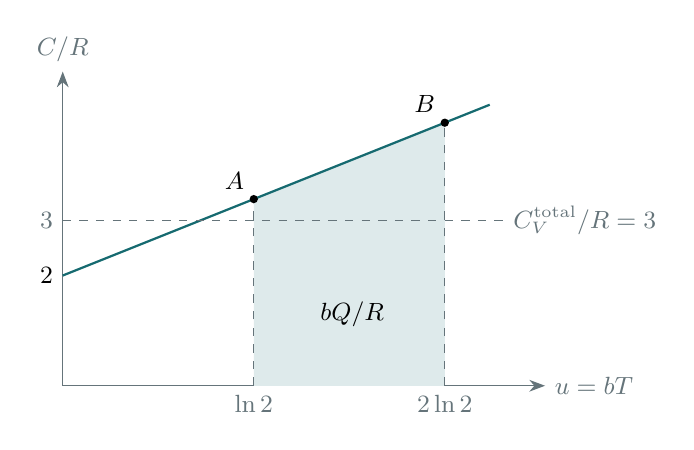
\begin{tikzpicture}[x=3.5cm,y=.7cm]
\draw[axis] (0,0)--(1.75,0) node[right] {$u=bT$};
\draw[axis] (0,0)--(0,5.7) node[above] {$C/R$};
\fill[accent!14] (.6931471806,0)--(.6931471806,3.3862943611)
--(1.3862943611,4.7725887222)--(1.3862943611,0)--cycle;
\node at (1.05,1.3) {$bQ/R$};
\draw[traj,domain=0:1.55,samples=60] plot (\x,{2*(1+\x)});
\draw[guide] (0,3) node[left] {$3$}--(1.6,3) node[right] {$C_V^{\rm total}/R=3$};
\node[left] at (0,2) {$2$};
\draw[guide] (.6931471806,0) node[below] {$\ln2$}--(.6931471806,3.3862943611);
\draw[guide] (1.3862943611,0) node[below] {$2\ln2$}--(1.3862943611,4.7725887222);
\fill (.6931471806,3.3862943611) circle(1.5pt) node[above left] {$A$};
\fill (1.3862943611,4.7725887222) circle(1.5pt) node[above left] {$B$};
\end{tikzpicture}\figcaption{解图 热2.6A　无量纲阴影面积为$bQ/R$；乘$R/b$给热量，内能增量以总定容热容量$3R$另算。}\end{minipage}\end{center}
\textbf{积分热量再作能量差。}图中梯形的无量纲面积为$bQ/R$；以物理温度为横坐标时，面积才直接等于$Q$。
\[\begin{aligned}
\Delta U&=3R(T_f-T_0)=3RT_0,\\
Q&=\int_{T_0}^{2T_0}2R(1+bT)\dd T
=2RT_0+3bRT_0^2,\\
W&=Q-\Delta U=RT_0(3bT_0-1).
\end{aligned}\]
取$R=8.314\,\mathrm{J/(mol\cdot K)}$，有
\result{\Delta U\approx1.729\times10^3\,\mathrm J,\qquad W\approx6.22\times10^2\,\mathrm J.}
由过程式$V/V_0=\exp[b(T-T_0)]\sqrt{T_0/T}$，可另求
\[\delta W=2RT\frac{\dd V}{V}=(2bRT-R)\dd T.\]
积分同得W。整个温区$T>1/(2b)=50\,\mathrm K$，所以体积随温度增加、功为正，满足给定终体积。
\subsubsection*{定量图上的截距、面积与体积分支}
图热2.6及解图热2.6A采用$u=bT$与$C/R$为坐标。
直线方程为$C/R=2(1+u)$，纵轴截距为2，而非零。
本题$u_0=\ln2$、$u_f=2\ln2$，端点热容量分别为
\[
\frac{C(T_0)}R=2+2\ln2\simeq3.38629,\qquad
\frac{C(2T_0)}R=2+4\ln2\simeq4.77259.
\]
温度翻倍不使热容量翻倍。总定容热容量为$3R$，在同一图中以水平虚线表示；
过程直线在整个题给温区都高于这条虚线，所以每次升温均有正的作功项。

阴影面积在所用无量纲坐标下等于
\[
\int_{u_0}^{2u_0}\frac CR\dd u
=2u_0+3u_0^2=\frac{bQ}{R}.
\]
乘上$R/b$后才是以焦耳计的热量。
因为$C(T)$确为一次函数，也可用梯形公式准确求出
\[
Q=\frac{C(T_0)+C(2T_0)}2(T_f-T_0)
=RT_0(2+3bT_0).
\]
梯形可分成以左端热容量为高的矩形和上方三角形。若把任一端点的热容量当成全程常量，矩形估算与精确热量的差的绝对值就是三角形面积 $bRT_0^2$。内能增加仍是$3RT_0$，与过程热容量的图形面积分开计算。

\begin{center}\begin{minipage}{0.96\linewidth}\centering
\begin{tikzpicture}[x=3.5cm,y=2cm]
\draw[axis] (0,0)--(1.7,0) node[right] {$u=bT$};
\draw[axis] (0,0)--(0,1.75) node[above] {$V/V_0$};
\draw[guide,domain=.3:.6931471806,samples=60]
 plot (\x,{exp(\x-.6931471806)*sqrt(.6931471806/\x)});
\draw[traj,domain=.6931471806:1.3862943611,samples=80]
 plot (\x,{exp(\x-.6931471806)*sqrt(.6931471806/\x)});
\draw[guide] (0,1) node[left] {$1$}--(.6931471806,1)--(.6931471806,0) node[below] {$\ln2$};
\draw[guide] (0,1.4142135624) node[left] {$\sqrt2$}--(1.3862943611,1.4142135624)--(1.3862943611,0) node[below] {$2\ln2$};
\fill[accent] (.6931471806,1) circle(1.5pt) node[above left] {$A$};
\fill[accent] (1.3862943611,1.4142135624) circle(1.5pt) node[above left] {$B$};
\fill (.5,.97061047422839) circle(1.4pt);
\draw[guide] (.5,.97061047422839)--(.5,.55) node[below] {$u=1/2$};
\draw[motion,domain=.95:1.1,samples=20] plot (\x,{exp(\x-.6931471806)*sqrt(.6931471806/\x)});
\end{tikzpicture}
\figcaption{解图 热2.6B　实线是本题$A\to B$的升温膨胀段；虚线是同一数学过程线在题给温区之外的延伸。}
\end{minipage}\end{center}
从过程式求得
\[
\frac{V}{V_0}=e^{b(T-T_0)}\sqrt{\frac{T_0}{T}},\qquad
\frac1V\frac{\dd V}{\dd T}=b-\frac1{2T}.
\]
解图热2.6B的极小体积出现在$u=1/2$，即50 K，
低于本题初温69.3147 K，故实际从$A$到$B$始终沿膨胀分支。
沿这段过程，$V$ 随 $T$ 增大，$\dd V>0$，因此气体对外做正功。

若保持同一路径而将端点温度比记作$r=T_f/T_0$、体积比记作$\lambda=V_f/V_0$，
则
\[
bT_0(r-1)=\ln\lambda+\frac12\ln r.
\]
在$r\ne1$时，
\[
T_0=\frac{\ln\lambda+\tfrac12\ln r}{b(r-1)}.
\]
给定的两个比例须对应 $T_0>0$。过程在各温度处膨胀或收缩，由 $b-1/(2T)$ 的符号确定。
本题$r=2,\lambda=\sqrt2$给$bT_0=\ln2$，两项对数各贡献一半。


\Needspace{18\baselineskip}

\pdfbookmark[2]{第 7 题 钢丝棉氧化反应中的热量与内能变化}{q7}

\section*{第 7 题\quad 钢丝棉氧化反应中的热量与内能变化}

空气中氮气、氧气的质量分数分别为76.9\%、23.1\%，其余成分忽略。气缸内装有空气和钢丝棉，活塞无摩擦地移动，使气压保持$1\,\mathrm{atm}$。在$300\,\mathrm K$下缓慢反应，生成1 mol $\mathrm{Fe_2O_3}$后，氧气恰耗尽；全过程向外释放$8.24\times10^5\,\mathrm J$热量。求系统内能变化、缸内气体内能变化和氮气密度变化。系统包括全部气体、铁及氧化物；固体体积忽略，氧气和氮气每摩尔内能均为$5RT/2$。

\begin{center}\begin{minipage}{0.96\linewidth}\centering
\begin{tikzpicture}[x=1cm,y=1cm]
\foreach \x/\h in {0/2.5256827048,5/2}{
 \fill[accent!7] (\x,0) rectangle ++(2.2,\h);
 \draw[object] (\x,3.15)--(\x,0)--++(2.2,0)--++(0,3.15);
 \draw[object,line width=2pt] (\x,\h)--++(2.2,0);
}
\node[align=center] at (1.1,1.3) {$\mathrm{N_2,O_2}$\\$V_i$};
\node[align=center] at (6.1,1.3) {$\mathrm{N_2}$\\$V_f\simeq0.792V_i$};
\node at (1.1,.25) {钢丝棉};
\node[align=center] at (6.1,.5) {$\mathrm{Fe_2O_3}$\\可有剩余铁};
\draw[guide] (5,2.5256827048)--(7.2,2.5256827048);
\draw[motion] (2.55,1.3)--(4.65,1.3);
\node[above,align=center] at (3.6,1.6) {恒温恒压\\反应};
\node[above] at (1.1,3.2) {初态};
\node[above] at (6.1,3.2) {末态};
\end{tikzpicture}\figcaption{图 热2.7　同一气缸的初、末状态分别画出；气相体积减小，钢丝棉只作符号示意。}\end{minipage}\end{center}

\Needspace{8\baselineskip}\subsection*{解答}

\textbf{总系统与气相分别求内能差。}解图热2.7A中氧气进入固体，氮气摩尔数不变。反应式为
\[2\mathrm{Fe}+\tfrac32\mathrm{O_2}\longrightarrow\mathrm{Fe_2O_3}.\]
生成1 mol氧化物恰消耗1.5 mol氧气，气相总摩尔数改变$\Delta\nu=-1.5\,\mathrm{mol}$。等温等压下
\[\Delta V=\Delta\nu RT/p_0,\qquad W=p_0\Delta V=-1.5RT=-3741.3\,\mathrm J.\]
\begin{center}\begin{minipage}{0.96\linewidth}\centering
\begin{tikzpicture}[x=1cm,y=1cm]
\foreach \x/\h in {0/2.5256827048,5/2}{
 \fill[accent!7] (\x,0) rectangle ++(2.2,\h);
 \draw[object] (\x,3.15)--(\x,0)--++(2.2,0)--++(0,3.15);
 \draw[object,line width=2pt] (\x,\h)--++(2.2,0);
}
\node[align=center] at (1.1,1.3) {$\mathrm{N_2,O_2}$\\$V_i$};
\node[align=center] at (6.1,1.3) {$\mathrm{N_2}$\\$V_f\simeq0.792V_i$};
\node at (1.1,.25) {钢丝棉};
\node[align=center] at (6.1,.5) {$\mathrm{Fe_2O_3}$\\可有剩余铁};
\draw[guide] (5,2.5256827048)--(7.2,2.5256827048);
\draw[motion] (2.55,1.3)--(4.65,1.3);
\node[above,align=center] at (3.6,1.6) {恒温恒压\\反应};
\node[above] at (1.1,3.2) {初态};
\node[above] at (6.1,3.2) {末态};
\draw[force] (6.1,-.1)--(6.1,-.95) node[below] {$Q=-8.24\times10^5\,\mathrm J$};
\node[below,align=center] at (1.1,-.2) {$\Delta\nu_{\rm gas}=-1.5\,\mathrm{mol}$\\$W=p_0\Delta V<0$};
\end{tikzpicture}\figcaption{解图 热2.7A　右筒的实线为末态、虚线为初始活塞高度；氧气进入固相，热向外传出。}\end{minipage}\end{center}
外界压缩系统，故对外功为负。总系统吸热$Q=-8.24\times10^5\,\mathrm J$，于是
\result{\Delta U_{\mathrm{tot}}=Q-W=-8.2026\times10^5\,\mathrm J.}
两种内能变化对应不同的对象。把气体与固体一起取为系统，反应释放的化学内能全部包含在$\Delta U_{\rm tot}$中；若只清点气相，按题给热运动内能模型，减少1.5 mol氧气便使气相内能减少。两者相减还能求固相的净变化：
\[\Delta U_{\rm solid}=\Delta U_{\rm tot}-\Delta U_{\rm gas}
\simeq-8.1091\times10^5\,\mathrm J.\]
解图热2.7A中温度保持不变，气相物质的量减少，固相中铁转为氧化物。这两种变化分别进入对应对象的内能差。

再求气相内能差。氮气量和温度不变，其内能不变；氧气量减少。按题给每摩尔内能，
\result{\Delta U_{\mathrm{gas}}=\tfrac52RT\Delta\nu=-9353.25\,\mathrm J.}
这里求的是气相初末内能差；题给$Q$对应全部反应物质。

\textbf{氮气密度。}初始氧气质量$M_O=1.5\times32=48\,\mathrm g$，氮气质量与摩尔数为
\[M_N=48\frac{76.9}{23.1}=159.7922\,\mathrm g,\qquad
\nu_N=\frac{159.7922}{28}=5.70686\,\mathrm{mol}.\]
初末体积
\[V_i=\frac{(\nu_N+1.5)RT}{p_0},\qquad V_f=\frac{\nu_NRT}{p_0}.\]
氮气初始分压$p_{N,i}=p_0\nu_N/(\nu_N+1.5)$，终态分压为$p_0$。用$\mu_N=0.028\,\mathrm{kg/mol}$，
\[\begin{aligned}
\Delta\rho_N&=\frac{M_N}{V_f}-\frac{M_N}{V_i}\\
&=\frac{\mu_Np_0}{RT}\frac{1.5}{\nu_N+1.5}
\approx0.2367\,\mathrm{kg/m^3}.
\end{aligned}\]
取$p_0=101325\,\mathrm{Pa}$。氮气的固定质量除以缩小后的气相总体积，得到较大的密度。初末两次计算的分子都取同一份氮气质量 $M_N$。
\subsubsection*{固定总系统、气相和氮气分别比较初末状态}
题中给出的放热量对应全部反应物质组成的封闭系统，
即氮气、氧气、铁和氧化物都放在活塞边界以内。
氧从气相进入固相时没有离开这一总系统，但离开了单独选取的气相。
所以总系统可以直接用$\Delta U_{\rm tot}=Q-W$，
气相内能则按两态的各组分摩尔数和题给的摩尔内能求差。

化学计量式表示每生成1 mol氧化物消耗2 mol铁和1.5 mol氧气。
氧气初量由产物数量确定；若初始铁多于反应所需量，剩余铁在相同温度下的内能贡献前后抵消。
解图热2.7A将气缸前后状态分开画出，末态气相只剩氮气，固相可同时含氧化物和剩余铁。
温度、总压强不变，但气相总摩尔数减少，因此
\[
\frac{V_f}{V_i}=\frac{\nu_N}{\nu_N+1.5}\simeq0.791865,\qquad
V_i-V_f=\frac{1.5RT}{p_0}\simeq0.0369238\,\mathrm{m^3}.
\]
活塞向内，系统对外功$W<0$，外界对总系统输入的机械功为$-W>0$。
外界的正压缩功补回一部分向外传出的热量，因此总内能下降的绝对值小于放热绝对值。

将三个研究对象并列，初、末内能变化分别为
\[
\begin{aligned}
\Delta U_{\rm tot}&=-824000+1.5RT=-820258.7\,\mathrm J,\\
\Delta U_{\rm gas}&=-\frac{15}{4}RT=-9353.25\,\mathrm J,\\
\Delta U_N&=0.
\end{aligned}
\]
差值给固相净变化$\Delta U_{\rm solid}=-810905.45\,\mathrm J$。
这些数值都取$R=8.314\,\mathrm{J/(mol\cdot K)}$与300 K。
总系统的变化还包含化学内能，气相的变化来自粒子数减少，氮气本身的内能不变；
三式分别跟随总系统、气相和氮气，使用各自初末状态求差。

\subsubsection*{氮气分压、共同体积与反应前后的密度}
初态两种气体均充满整个体积$V_i$，各自的分压满足该组分的理想气体状态方程。
初态分压关系完整写成
\[
p_{N,i}V_i=\nu_NRT,\qquad
(p_0-p_{N,i})V_i=1.5RT.
\]
相加求初始总容积；末态纯氮满足$p_0V_f=\nu_NRT$。
密度也可直接由分压写成
\[
\rho_{N,i}=\frac{\mu_Np_{N,i}}{RT},\qquad
\rho_{N,f}=\frac{\mu_Np_0}{RT}.
\]
用题给质量分数先换摩尔数，所得初态氧摩尔分数约为0.208135，由氧和氮各自的质量除摩尔质量后求比得到。由此
\[
p_{N,i}\simeq80235.7\,\mathrm{Pa},\quad
\rho_{N,i}\simeq0.900730\,\mathrm{kg/m^3},\quad
\rho_{N,f}\simeq1.137479\,\mathrm{kg/m^3}.
\]
二者相减给$0.236749\,\mathrm{kg/m^3}$，与同一氮气质量除初、末体积所得结果一致。
氮气的质量和摩尔数在反应前后保持；其分压由混合气体总压与摩尔分数确定，密度则由这份固定质量除以各状态的体积得到。


\Needspace{18\baselineskip}

\pdfbookmark[2]{第 8 题 双活塞气缸加热的分段末温}{q8}

\section*{第 8 题\quad 双活塞气缸加热的分段末温}

固定直立气缸由相连通的上下圆筒构成。上筒容积$V_m$，其中薄活塞A质量$2m$、面积$2S$；足够长的下筒有活塞B，质量$m$、面积$S$。A上方有1 mol理想气体，A、B之间有另一气体，B下方与压强$p_0$的大气连通。两活塞无摩擦、不漏气；筒壁、短连接管和活塞均绝热。初态平衡，A上方温度$T_0$，每摩尔内能$U=CT$，$C$为常量。通过顶部电热丝向A上方气体缓慢输入热量$Q_0\ge0$，求终态温度$T_f$，讨论A是否到达上筒底端的各种情况。取$p_0>2mg/S$。

\begin{center}\begin{minipage}{0.96\linewidth}\centering
\begin{tikzpicture}[x=1cm,y=1cm,font=\small]\draw[object] (0,4)--(0,1.8)--(.6,1.8)--(.6,0);\draw[object] (2,4)--(2,1.8)--(1.6,1.8)--(1.6,0);\draw[object] (0,4)--(2,4);\fill[accent!8] (0,2.6) rectangle(2,4);\draw[object,line width=2pt] (0,2.6)--(2,2.6);\draw[object,line width=2pt] (.6,.7)--(1.6,.7);\node at (1,3.3){$T,V$};\node[right] at (2.15,2.6){A：$2m,2S$};\node[right] at (2.15,.7){B：$m,S$};\node[below] at (1,0){大气$p_0$};\draw[force] (1,4.6)--(1,3.8) node[pos=0,left]{$Q_0$};
\end{tikzpicture}\figcaption{图 热2.8　A向下移动使其上方气体膨胀，A到上筒底端后体积固定。}\end{minipage}\end{center}

\Needspace{8\baselineskip}\subsection*{解答}

\textbf{先由两活塞平衡确定移动段压强。}解图热2.8A中B下受大气向上作用，上受中间气体和自重向下作用；A下受中间气体向上作用，上受待加热气体和自重向下作用。未碰底时
\[p_2S+mg=p_0S,\qquad 2Sp_1+2mg=2Sp_2.\]
因此
\[p_2=p_0-mg/S,\qquad p_1=p_*=p_0-2mg/S>0.\]
A向下移动使上方气体膨胀，直到其体积达到$V_m$。定义
\[T_*=\frac{p_*V_m}{R}.\]
\begin{center}\begin{minipage}{0.96\linewidth}\centering
\begin{tikzpicture}[x=1cm,y=1cm,font=\small]\draw[object] (0,4)--(0,1.8)--(.6,1.8)--(.6,0);\draw[object] (2,4)--(2,1.8)--(1.6,1.8)--(1.6,0);\draw[object] (0,4)--(2,4);\fill[accent!8] (0,2.6) rectangle(2,4);\draw[object,line width=2pt] (0,2.6)--(2,2.6);\draw[object,line width=2pt] (.6,.7)--(1.6,.7);\node at (1,3.3){$T,V$};\node[right] at (2.15,2.6){A：$2m,2S$};\node[right] at (2.15,.7){B：$m,S$};\node[below] at (1,0){大气$p_0$};\draw[force] (1,4.6)--(1,3.8) node[pos=0,left]{$Q_0$};\node[left] at (-.2,3){$p_*=p_0-2mg/S$};\node[left] at (-.2,1.5){$p_2=p_0-mg/S$};\draw[force] (3.5,2.3)--(3.5,1.6) node[right,midway]{$2mg$};
\end{tikzpicture}\figcaption{解图 热2.8A　分别对A、B列力平衡；各支压力按相应活塞面积计算。}\end{minipage}\end{center}
\textbf{初态已碰底。}若$T_0\ge T_*$，A已在底端，接触反力承担多余压差。加热全程等容，$W=0$，
\[Q_0=C(T_f-T_0),\qquad T_f=T_0+Q_0/C.\]
\textbf{初态可移动。}若$T_0<T_*$，初始$V_0=RT_0/p_*<V_m$。碰底前等压，有
\[W=p_*(V-V_0)=R(T-T_0),\qquad
Q=(C+R)(T-T_0).\]
刚碰底时$T=T_*$，所需热量
\[Q_*=(C+R)(T_*-T_0).\]
若$0\le Q_0\le Q_*$，全程等压（等号时恰碰底），$T_f=T_0+Q_0/(C+R)$。

若$Q_0>Q_*$，先等压到$T_*$，再等容加热：
\[Q_0=Q_*+C(T_f-T_*),\qquad
T_f=T_*+\frac{Q_0-Q_*}{C}.\]
将临界量代回，也可写为$[Q_0-p_*V_m+(C+R)T_0]/C$。
\begin{center}\begin{minipage}{0.96\linewidth}\centering
\begin{tikzpicture}[x=2cm,y=.9cm]
\draw[axis] (0,0)--(3.3,0) node[right] {$q=Q/Q_*$};
\draw[axis] (0,0)--(0,4.2) node[above] {$\theta=(T-T_0)/(T_*-T_0)$};
\draw[traj] (0,0)--(1,1)--(2.5,3.5);
\draw[traj,warm] (1,1)--(2.5,3.1);
\draw[guide] (1,0) node[below] {$1$}--(1,1)--(0,1) node[left] {$1$};
\fill[accent] (1,1) circle(1.7pt);
\node at (.35,1.55) {$\theta=q$};
\node[right] at (2.55,3.5) {$C/R=3/2$};
\node[right] at (2.55,3.05) {$C/R=5/2$};
\end{tikzpicture}\figcaption{解图 热2.8B　未碰底初态的归一化加热曲线；两种热容量示例都在$(1,1)$转折，碰底后斜率增大。}\end{minipage}\end{center}
\result{T_f=\begin{cases}
T_0+Q_0/C,&T_0\ge T_*,\\
T_0+Q_0/(C+R),&T_0<T_*,\ Q_0\le Q_*,\\
T_*+(Q_0-Q_*)/C,&T_0<T_*,\ Q_0>Q_*.
\end{cases}}
解图热2.8B中的温度曲线在碰底处连续，之后的斜率变大，对应等压段转为等容段。第三式与第二式在$Q_0=Q_*$时均给出$T_*$，且$Q_0\to0$均回到初温。底端限制使等压段结束、等容段开始，热容量相应由$C+R$变为$C$。
\subsubsection*{自由移动时的受力平衡与碰底后的支承力}
对活塞$B$，向上的压力为$p_0S$，向下为$p_2S$与$mg$；
对自由活塞$A$，向上为$2Sp_2$，向下为$2Sp_1$与$2mg$。
先由 $B$ 的平衡求 $p_2=p_0-mg/S$，再将此压强代入 $A$ 的平衡，得到待加热气体的压强 $p_1=p_*$。
题设$p_0>2mg/S$保证自由段的$p_*>0$。

\begin{center}\begin{minipage}{0.96\linewidth}\centering
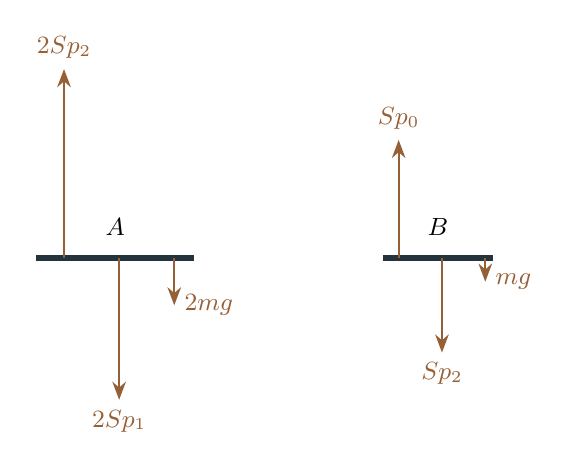
\begin{tikzpicture}[x=1cm,y=1cm]
\draw[object,line width=2pt] (0,1)--(2,1);
\node at (1,1.4) {$A$};
\draw[force] (.35,1)--(.35,3.4) node[above] {$2Sp_2$};
\draw[force] (1.05,1)--(1.05,-.8) node[below] {$2Sp_1$};
\draw[force] (1.75,1)--(1.75,.4) node[right] {$2mg$};
\draw[object,line width=2pt] (4.4,1)--(5.8,1);
\node at (5.1,1.4) {$B$};
\draw[force] (4.6,1)--(4.6,2.5) node[above] {$Sp_0$};
\draw[force] (5.15,1)--(5.15,-.2) node[below] {$Sp_2$};
\draw[force] (5.7,1)--(5.7,.7) node[right] {$mg$};
\end{tikzpicture}
\figcaption{解图 热2.8C　自由移动时的受力。按 $p_0=5mg/S$ 画箭头，两个活塞各自的向上力与两项向下力平衡。}
\end{minipage}\end{center}
当 $A$ 碰底时，上方体积达到几何上限 $V_m$。令支承反力为$N\ge0$，平衡式变为
\[
2Sp_2+N=2Sp_1+2mg,\qquad N=2S(p_1-p_*).
\]
自由时$N=0$给$p_1=p_*$；碰底后可有$p_1>p_*$，多出的压力由支承力平衡。
初态若$T_0\ge T_*$，在$V_m$内的压强为$RT_0/V_m\ge p_*$，
故支承力非负，初始状态就在底端，几何约束由这支反力维持。
若$T_0<T_*$，初始自由体积$RT_0/p_*$小于$V_m$，存在实际的等压移动段。

\subsubsection*{碰底所需的临界热量与分段能量关系}
初态未碰底时，对任一未接触状态有
\[
p_*V=RT,\qquad p_*V_0=RT_0,\qquad
p_*(V-V_0)=R(T-T_0).
\]
第一定律逐项给
\[
Q=C(T-T_0)+p_*(V-V_0)=(C+R)(T-T_0).
\]
将$V$解出来，更便于判定是否达到限位：
\[
V=\frac R{p_*}\left(T_0+\frac Q{C+R}\right).
\]
$V\le V_m$等价于$Q\le(C+R)(p_*V_m/R-T_0)=Q_*$；
这一步把几何条件转成题给输入热量可直接比较的条件。

若越过临界，整个过程的功在碰底后不再增加，其总值为
\[
W_{\rm tot}=p_*(V_m-V_0)=R(T_*-T_0).
\]
把碰底前的总功代入全程热力学第一定律，
\[
\begin{aligned}
Q_0&=C(T_f-T_0)+R(T_*-T_0),\\
T_f&=\frac{Q_0-RT_*+(C+R)T_0}{C}
=T_*+\frac{Q_0-Q_*}{C}.
\end{aligned}
\]
该式把碰底前的膨胀功与全程内能变化相加，直接给出越过临界热量后的末温。
若初态已碰底，则$W_{\rm tot}=0$，同一第一定律给$T_f=T_0+Q_0/C$。

解图热2.8B只适用于$T_0<T_*$的起点。用
$q=Q/Q_*$、$\theta=(T-T_0)/(T_*-T_0)$表示，曲线为
\[
\theta=q\quad(0\le q\le1),\qquad
\theta=1+\frac{C+R}{C}(q-1)\quad(q>1).
\]
图中分别以$C=3R/2$与$5R/2$展示后段斜率，转折点都在$(1,1)$；
一般$C>0$时，前段实际导数为$1/(C+R)$，后段为$1/C$。
温度连续，但导数跳变，表示加热时膨胀功的支出停止。
$Q_0=0$时末温保持初温；$Q_0=Q_*$时恰到限位温度$T_*$；$T_0=T_*$时初态已位于底端，随后沿等容段升温。
\subsubsection*{三类初态和热量条件怎样实际选用}
给定参数$T_0,Q_0,V_m,p_0,m/S$共同决定初始位置和最终接触状态，各分支按这些参数的大小关系选取。
先求$T_*$，是把初态位置判定转成已知温度的比较；
再求$Q_*$，才把加热后的接触判定转成已知热量的比较。
先按$T_0$与$T_*$比较初态位置。$T_0\ge T_*$时活塞从底端开始，加热沿等容段进行；$T_0<T_*$时存在等压移动段，再按$Q_0$与正的$Q_*$比较末态位置。
两种气体之间不导热，取上方气体为热力学系统，输入热量为题给$Q_0$，内能变化为$C(T_f-T_0)$，对外传递的能量通过膨胀功计入。

以下选解图热2.8B中的单原子示例，令$C=3R/2$、$R=8.314$，
并取装置参数使$T_*=300\,\mathrm K$。
以下三个初温、热量组合分别对应初态已碰底、加热中保持自由移动以及加热后碰底的过程。
先取$T_0=400\,\mathrm K$，输入$Q_0=1247.1\,\mathrm J$。
初温已经大于临界温度，活塞从受支承状态开始，
\[
T_f=400+\frac{1247.1}{12.471}=500\,\mathrm K,\qquad
W=0,\quad \Delta U=1247.1\,\mathrm J.
\]
没有等压段，末压比初压提高到$500/400$，
支承力随温度和压强一同增加，所输入的热量全部用于内能增加。

再取自由初态$T_0=150\,\mathrm K$。
到限位的温差为150 K，故
\[
Q_*=(C+R)(300-150)=3117.75\,\mathrm J.
\]
若只输入$2078.5\,\mathrm J<Q_*$，则
\[
T_f=150+\frac{2078.5}{20.785}=250\,\mathrm K,\qquad
\frac{V_f}{V_m}=\frac{T_f}{T_*}=\frac56<1.
\]
活塞尚未碰底，$N=0$；
内能增加$1247.1\,\mathrm J$，作功$831.4\,\mathrm J$，两者相加等于输入热量。
末体积仍小于挡块所限定的体积，活塞在整段中保持自由移动。

保持同一自由初态，将热量增至$4988.4\,\mathrm J>Q_*$。
先到300 K，再以剩余热量$1870.65\,\mathrm J$等容升温，
\[
T_f=300+\frac{1870.65}{12.471}=450\,\mathrm K.
\]
全程功仍只有碰底前的$R(300-150)=1247.1\,\mathrm J$，
内能增加$C(450-150)=3741.3\,\mathrm J$，
和为$4988.4\,\mathrm J$。末体积等于$V_m$、末压为$1.5p_*$，
因此解图热2.8C中的 $A$ 受到正的向上支承力。
三个算例分别对应不同的初态位置与输入热量。自由移动时，一部分热量用于膨胀功，温度变化按$C+R$计算；碰底后膨胀停止，温度变化按$C$计算。



\Needspace{18\baselineskip}

\pdfbookmark[2]{第 9 题 绝热压缩后缓慢扩散的终温}{q9}

\section*{第 9 题\quad 绝热压缩后缓慢扩散的终温}

两个对外绝热容器A、B经短细管相连，阀门K导热良好，活塞F绝热、无摩擦、不漏气；装置热容量忽略。初始K关，A内有$n$ mol理想气体，温度$T_0$，B为真空。推F将A中气体压缩到与B容积相等，外界作功$W$，温度升为$T_1$。再稍开K，使气体缓慢流入B，同时缓慢推F，保持F附近气压近似不变。直到两容器达到共同平衡，求终温。气体定容摩尔热容量为常量。

\begin{center}\begin{minipage}{0.96\linewidth}\centering
\begin{tikzpicture}[x=1cm,y=1cm]
\fill[accent!7] (.4,0) rectangle (3.4,1.8);
\draw[object] (-.6,1.8)--(3.4,1.8)--(3.4,1.05);
\draw[object] (-.6,0)--(3.4,0)--(3.4,.75);
\draw[object] (4.4,1.05)--(4.4,1.8)--(7.4,1.8)--(7.4,0)--(4.4,0)--(4.4,.75);
\draw[object] (3.4,.75)--(4.4,.75) (3.4,1.05)--(4.4,1.05);
\draw[object,line width=2pt] (.4,0)--(.4,1.8);
\draw[object] (-1.2,.9)--(.4,.9);
\node[above] at (-.8,.9) {$F$};
\draw[object] (3.9,.75)--(3.9,1.05);
\node[above] at (3.9,1.15) {$K$};
\node[align=center] at (1.9,.9) {$A$\\$n,T_1,V_1$};
\node[align=center] at (5.9,.9) {$B$\\真空，$V_1$};
\end{tikzpicture}\figcaption{图 热2.9　第一阶段结束后，A、B几何容积相等，B仍为真空。}\end{minipage}\end{center}

\Needspace{8\baselineskip}\subsection*{解答}

\textbf{第一阶段确定热容量。}整体对外绝热，第一阶段外界对气体作功W，故
\[W=nC_V(T_1-T_0),\qquad C_V=\frac{W}{n(T_1-T_0)}.\]
记B容积为$V_1$，第二阶段开始时A也为$V_1$，A内气压$p=nRT_1/V_1$。解图热2.9A中阀门小开，活塞附近气压保持p，外界功按$p$乘活塞扫过体积计算；流入初始真空区的气体同时经历不可逆扩散。
\begin{center}\begin{minipage}{0.96\linewidth}\centering
\begin{tikzpicture}[x=1cm,y=1cm]
\fill[accent!7] (2.2,0) rectangle (3.4,1.8);
\draw[object] (-.6,1.8)--(3.4,1.8)--(3.4,1.05);
\draw[object] (-.6,0)--(3.4,0)--(3.4,.75);
\fill[accent!7] (4.4,0) rectangle (7.4,1.8);
\draw[object] (4.4,1.05)--(4.4,1.8)--(7.4,1.8)--(7.4,0)--(4.4,0)--(4.4,.75);
\draw[object] (3.4,.75)--(4.4,.75) (3.4,1.05)--(4.4,1.05);
\draw[object,line width=2pt] (2.2,0)--(2.2,1.8);
\draw[object] (-.6,.9)--(2.2,.9);
\node[above] at (-.8,.9) {$F$};
\draw[object] (3.8,.73)--(4,1.07);
\node[above] at (3.9,1.15) {$K$};
\node[align=center] at (2.8,.9) {$A$\\$T_2,V^\prime$};
\node[align=center] at (5.9,.9) {$B$\\$T_2,V_1$};
\draw[guide] (.4,0)--(.4,1.8);
\draw[motion] (.7,2.2)--(1.9,2.2) node[midway,above] {外活塞右移};
\node[below] at (3.9,-.4) {初始气体占据$V_1$；末态占据$V_1+V^\prime$};
\end{tikzpicture}\figcaption{解图 热2.9A　末态两室同温同压。图取单原子气体，A 室末体积为 $2V_1/5$。虚线和实线分别是活塞 $F$ 的初位和末位。}\end{minipage}\end{center}
\textbf{末态还留有A中气体。}设终态A内体积$V'$、共同温度$T_2$。平衡时B的气压等于A的p，总状态方程为
\[p(V_1+V')=nRT_2.\]
与初态$pV_1=nRT_1$相减，得
\[pV'=nR(T_2-T_1).\]
活塞从$V_1$压到$V'$，外界作功$W'=p(V_1-V')$。对两室全部气体列第一定律：
\[p(V_1-V')=nC_V(T_2-T_1).\]
将$pV_1=nRT_1$及$pV'$代入，
\[nRT_1=n(C_V+R)(T_2-T_1),\qquad
T_2=\frac{C_V+2R}{C_V+R}T_1.\]
\Needspace{10\baselineskip}
\result{T_2=\frac{W+2nR(T_1-T_0)}{W+nR(T_1-T_0)}T_1.}
由前式还得
\[\frac{V'}{V_1}=\frac{R}{C_V+R},\qquad
W'=nRT_1\frac{C_V}{C_V+R}.\]
$V^{\prime}>0$ 且 $T_1<T_2<2T_1$，末态两室均有气体。活塞输入的正功使总内能增加，终温高于开阀前温度。
\subsubsection*{三个体积与两个独立方程}
第二阶段开始时，气体实际只占$A$的$V_1$，
而装置中可以被气体占据的总空间为$2V_1$，其中$B$还是空的。
末态$A$剩余$V'$，$B$几何容积始终为$V_1$，
气体占据的总体积和装置剩余可用体积都为$V_1+V'$。
因此气体占据体积从$V_1$增大到$V_1+V'$，
外活塞同时向内扫去体积 $V_1-V^{\prime}>0$，提供压缩功。
解图热2.9A的$F$是外部活动边界，阀$K$是两室之间的内部通路，
外界通过 $F$ 输入的功按它扫过的体积 $V_1-V^{\prime}$ 计算。

由第一阶段得$C_V=W/[n(T_1-T_0)]$，要求$W>0,T_1>T_0$。
记第二阶段初压为$p$，逐步比较初、末平衡态：
\[
pV_1=nRT_1,\qquad p(V_1+V')=nRT_2,
\]
所以
\[
pV'=nR(T_2-T_1).
\]
另一方面，两室全部气体组成的固定系统对外绝热，
活塞受压为$p$，故
\[
W'_{\rm in}=\int_{V'}^{V_1}p\dd V_A=p(V_1-V'),
\qquad nC_V(T_2-T_1)=W'_{\rm in}.
\]
从后一式也得到
$pV'=nRT_1-nC_V(T_2-T_1)$。
将这两个 $pV^{\prime}$ 相等，整体的能量与末态状态方程给出温升
\[
(C_V+R)(T_2-T_1)=RT_1,\qquad
T_2-T_1=\frac{R}{C_V+R}T_1.
\]
阀门导热良好、等待充分平衡使两室最终同温，但没有外界热量输入。

由 $C_V>0$，剩余体积比例 $R/(C_V+R)$ 介于0和1之间。末态同压同温，摩尔数按两室体积配分，因此有
\[
\frac{V'}{V_1}=\frac{R}{C_V+R},\qquad
\frac{n_{A,f}}n=\frac{R}{C_V+2R},\qquad
\frac{n_{B,f}}n=\frac{C_V+R}{C_V+2R}.
\]


例如单原子气体$C_V=3R/2$时，
$T_2=7T_1/5,V'=2V_1/5$，两室分别留有$2n/7$与$5n/7$，
输入功为$3nRT_1/5$。此时总占气体积为 $7V_1/5$，温度同样变为 $7T_1/5$，压强保持；输入的 $3nRT_1/5$ 全部成为内能增加。
整个过程含向初始真空区的不可逆扩散，其总熵增为
\[
\Delta S=nC_V\ln\frac{T_2}{T_1}
+nR\ln\frac{V_1+V'}{V_1}
=n(C_V+R)\ln\frac{C_V+2R}{C_V+R}>0.
\]
装置整体对外绝热，能量由外界推动活塞输入。气体向初始真空区扩散产生正熵增，两个平衡态由总能量和状态方程联系。


\Needspace{18\baselineskip}

\pdfbookmark[2]{第 10 题 带阀绝热活塞与电热器的能量分配}{q10}

\section*{第 10 题\quad 带阀绝热活塞与电热器的能量分配}

刚性封闭绝热圆筒内装有带阀门L的绝热活塞，左端A装电热器H。初始活塞紧贴右端B内壁，L关，气体温度$T_0$。将活塞推到中央并固定，外界对气体作功$W$，温度升为$T$；右半为真空。开L，充分平衡后关L，再解除固定，活塞无摩擦地自由移动。加热后，左室压强为加热前的1.5倍，右室体积为加热前的0.75倍。求电热器输入的能量$Q$。气体内能正比于温度；初末活塞均静止。

\begin{center}\begin{minipage}{0.96\linewidth}\centering
\begin{tikzpicture}[x=1cm,y=1cm,font=\small]\draw[object,fill=accent!6] (0,0) rectangle (6,1.8);\draw[object,line width=2pt] (6,0)--(6,1.8);\node[align=center] at (2.9,.9) {气体\\$T_0$};\node[align=center] at (5.9,.9) {};\node[above] at (6,2.1){活塞L关};\draw[force] (.4,-.7)--(.4,.1) node[pos=0,below]{H};
\end{tikzpicture}\figcaption{图 热2.10　起始气体占据整个圆筒，电热器位于左端。}\end{minipage}\end{center}

\Needspace{8\baselineskip}\subsection*{解答}

\textbf{三个阶段开始时的状态。}设全部气体内能$U=kT$。从初态到活塞被固定在中央，装置绝热，故
\[W=k(T-T_0),\qquad k=\frac{W}{T-T_0}.\]
开阀时外边界刚性、活塞固定，气体向右半真空自由膨胀，$Q=W_{\mathrm{out}}=0$。理想气体内能和温度不变；足够久后两半同温T、同压p、同体积V，因此各有一半摩尔数。
\begin{center}\begin{minipage}{0.96\linewidth}\centering
\begin{tikzpicture}[x=1cm,y=1cm]
\foreach \y/\xp/\state in {5.8/3/{压缩后：$L$关，活塞固定},2.9/3/{开阀平衡后再关阀},0/3.75/{加热末态：$L$关}}{
 \draw[object] (0,\y) rectangle ++(6,1.8);
 \draw[object,line width=2pt] (\xp,\y)--++(0,1.8);
 \node[right,align=left] at (6.2,\y+.9) {\state};
}
\fill[accent!7] (0,5.8) rectangle (3,7.6);
\draw[object] (0,5.8) rectangle (6,7.6);
\draw[object,line width=2pt] (3,5.8)--(3,7.6);
\node[align=center] at (1.5,6.7) {$A:T,V$\\$p_A=2p$};
\node[align=center] at (4.5,6.7) {$B$真空\\$V$};
\fill[accent!7] (0,2.9) rectangle (6,4.7);
\draw[object] (0,2.9) rectangle (6,4.7);
\draw[object,line width=2pt] (3,2.9)--(3,4.7);
\node[align=center] at (1.5,3.8) {$A:T,V,p$\\$n/2$};
\node[align=center] at (4.5,3.8) {$B:T,V,p$\\$n/2$};
\fill[warm!7] (0,0) rectangle (3.75,1.8);
\fill[accent!7] (3.75,0) rectangle (6,1.8);
\draw[object] (0,0) rectangle (6,1.8);
\draw[object,line width=2pt] (3.75,0)--(3.75,1.8);
\node[align=center] at (1.875,.9) {$T_A,5V/4$\\$p_A=3p/2$};
\node[align=center] at (4.875,.9) {$T_B,3V/4$\\$p_B=3p/2$};
\draw[force] (-1,.9)--(.2,.9) node[pos=0,left] {$Q$};
\end{tikzpicture}\figcaption{解图 热2.10A　三阶段分别对应外界压缩作功、自由膨胀和电热输入。}\end{minipage}\end{center}
解图热2.10A中，压缩时活塞向气体输入功，开阀时刚性外壳及固定活塞保持，最后由电热丝输入能量。图中末态A、B两室容积分别为$5V/4$和$3V/4$，相加仍是$2V$；末态的共同压强与各自的末体积相乘，分别给两份固定摩尔数气体的温度。

\textbf{关阀后两室量分别守恒。}最终右室为$3V/4$，总容积$2V$固定，左室为$5V/4$。活塞末态平衡，两室压强均$3p/2$。分别列状态方程：
\[\frac{T_A}{T}=\frac{(3p/2)(5V/4)}{pV}=\frac{15}{8},\qquad
\frac{T_B}{T}=\frac{(3p/2)(3V/4)}{pV}=\frac98.\]
每室内能系数为$k/2$，故
\[\Delta U_A=\frac{k}{2}\frac{7T}{8}=\frac{7kT}{16},\qquad
\Delta U_B=\frac{k}{2}\frac{T}{8}=\frac{kT}{16}.\]
右室虽没电热器，仍因被压缩而升温。左室对右室的功属于内部交换；整个刚性装置无外边界功，初末活塞动能均零。因此输入电能等于总内能增加：
\result{Q=\Delta U_A+\Delta U_B=\frac{kT}{2}=\frac{WT}{2(T-T_0)}.}
由初末静止状态与整体能量即可求出输入能量。右室的初末态还满足封闭绝热系统的熵不减条件，下面由此确定热容量的范围。
\subsubsection*{三次操作中各守恒什么}
第一次在阀关闭时推活塞，固定的是总气体量，外界功使总内能由$kT_0$增至$kT$。
第二次将活塞固定、打开阀门，外壳不变形且没有外热交换，
因此总内能仍为$kT$，理想气体温度仍为$T$。
充分平衡后两室同压、同温、同体积，状态方程才保证各含一半摩尔数。
第三次先关阀再解除固定，从这一刻起左右摩尔数分别守恒；
关阀后每室气体量固定，内能系数各为 $k/2$。

解图热2.10A的末态，右室体积减少$V/4$，
刚性外筒的总体积固定，左室增加同样的量，故 $V_A=5V/4,V_B=3V/4$。
两份固定量的气体分别满足各自的状态比例式，得
\[
\frac{pV}{T}=\frac{(3p/2)(5V/4)}{T_A},\qquad
\frac{pV}{T}=\frac{(3p/2)(3V/4)}{T_B}.
\]
于是$T_A=15T/8,T_B=9T/8$，两室末温不同，
这与绝热活塞允许机械平衡而不传热相容。
总内能为
\[
U_f=\frac k2T_A+\frac k2T_B=\frac32kT,\qquad
Q=U_f-U_{\rm heat,i}=\frac12kT.
\]
加热阶段从开阀平衡后的状态开始，初态内能为 $U_{\rm heat,i}=kT$；
计算电热输入时应从开阀平衡后的状态开始。

\begin{center}\begin{minipage}{0.96\linewidth}\centering
\begin{tikzpicture}[x=1cm,y=1cm]
\node[draw,minimum width=2.6cm,minimum height=1.5cm,align=center] (A) at (0,0)
 {左室$A$\\$\Delta U_A=7kT/16$};
\node[draw,minimum width=2.6cm,minimum height=1.5cm,align=center] (B) at (5,0)
 {右室$B$\\$\Delta U_B=kT/16$};
\draw[force] (-4.6,0)--(A.west) node[midway,above] {$Q=8kT/16$};
\draw[motion] (A.east)--(B.west);
\draw[guide] (2.5,.05)--(2.5,.85);
\node[above] at (2.5,.85) {$W_{A\to B}=kT/16$};
\node[below] at (2.5,-1.1) {活塞的功在两室整体中相消};
\end{tikzpicture}
\figcaption{解图 热2.10B　加热阶段的电能输入、两室内能增加与内部传功。}
\end{minipage}\end{center}
右室没有加热器，也不经壁或活塞受热，它的内能增加来自活塞的输入功，
所以$W_{\rm in,B}=\Delta U_B=kT/16$。
活塞初末静止，其对左右气体传递的功在整体方程中相消，
左室有$Q=\Delta U_A+W_{\rm out,A}=8kT/16$。
解图热2.10B的两个局部方程相加，内部传功相消，留下输入能量和两室内能增加之和。

\subsubsection*{右室熵变与热容量的范围}
右室是封闭绝热子系统，给定初、末状态的熵变化应满足绝热过程的熵增条件。
设全部气体共有$n$ mol，定容摩尔热容量为常量$C_V=k/n$。
关阀后的右室是封闭绝热子系统，故应有
\[
\Delta S_B=\frac n2\left[
C_V\ln\frac98+R\ln\frac34\right]\ge0.
\]
因此必要条件为
\[
\frac{C_V}{R}\ge
\frac{\ln(4/3)}{\ln(9/8)}
\simeq2.442475.
\]
常温双原子模型$C_V/R=5/2$可满足这个不等式，
单原子模型 $C_V/R=3/2$ 代入该式得到负熵变，给定的这组末态对应于上述允许热容量范围。
等号对应右室可逆绝热，所需指数为
\[
\gamma_{\rm eq}=
\frac{\ln(3/2)}{\ln(4/3)}
\simeq1.409421.
\]
若实际$C_V$更大，右室可有正熵产生；该必要条件本身不指定沿途的具体活塞运动。
给定末态在能量上确定 $Q$，熵变条件则进一步限定可采用的气体热容量；具体的活塞运动由加热和力学过程决定。


\Needspace{18\baselineskip}

\pdfbookmark[2]{第 11 题 绝热左筒与等温右筒的活塞平衡}{q11}

\section*{第 11 题\quad 绝热左筒与等温右筒的活塞平衡}

两个圆筒截面积均为$S=100\,\mathrm{cm^2}$，活塞用轻杆相连，外部为真空。左筒绝热，内有同种理想气体$4\,\mathrm g$，初始$22.4\,\mathrm L$、$1\,\mathrm{atm}$、$273\,\mathrm K$；右筒有$7.44\,\mathrm g$，初始$22.4\,\mathrm L$、$273\,\mathrm K$，靠大热库保持$273\,\mathrm K$。放开活塞后，移动$50\,\mathrm{cm}$并最终静止。摩擦忽略，气体定容比热$c_V=3.14\,\mathrm{J/(g\cdot K)}$。求右筒从热库吸收的热量。

\begin{center}\begin{minipage}{0.96\linewidth}\centering
\begin{tikzpicture}[x=1cm,y=1cm]
\fill[accent!8] (0,0) rectangle (2.24,1.8);
\fill[warm!7] (4.96,0) rectangle (7.2,1.8);
\draw[object] (3.1,1.8)--(0,1.8)--(0,0)--(3.1,0);
\draw[object] (4.1,1.8)--(7.2,1.8)--(7.2,0)--(4.1,0);
\draw[object,line width=2pt] (2.24,0)--(2.24,1.8) (4.96,0)--(4.96,1.8);
\draw[object] (2.24,.9)--(4.96,.9);
\node[align=center] at (1.12,.9) {左：绝热\\4 g，273 K};
\node[align=center] at (6.08,.9) {右：等温\\7.44 g，273 K};
\node[above] at (1.12,1.95) {$V_0=22.4\,\mathrm L$};
\node[above] at (6.08,1.95) {$V_0=22.4\,\mathrm L$};
\draw[motion] (3.85,1.3)--(3.35,1.3) node[midway,above] {$0.50\,\mathrm m$};
\node[below] at (3.6,-.2) {相连活塞同时左移，杆长不变};
\end{tikzpicture}\figcaption{图 热2.11　杆连活塞一起向左移动：左气体压缩，右气体膨胀。}\end{minipage}\end{center}

\Needspace{8\baselineskip}\subsection*{解答}

\textbf{方向与几何。}两室同种气体、初温和初体积相等，所以
\[p_{R,i}/p_{L,i}=M_R/M_L=7.44/4=1.86.\]
右筒推动相连活塞向左，左气体被压缩。解图热2.11A中位移使体积改变
\[Sl=100\times10^{-4}\times0.50=0.0050\,\mathrm{m^3}=5.0\,\mathrm L.\]
\begin{center}\begin{minipage}{0.96\linewidth}\centering
\begin{tikzpicture}[x=1cm,y=1cm]
\fill[accent!8] (0,0) rectangle (1.74,1.8);
\fill[warm!7] (4.46,0) rectangle (7.2,1.8);
\draw[object] (3.1,1.8)--(0,1.8)--(0,0)--(3.1,0);
\draw[object] (4.1,1.8)--(7.2,1.8)--(7.2,0)--(4.1,0);
\draw[object,line width=2pt] (1.74,0)--(1.74,1.8) (4.46,0)--(4.46,1.8);
\draw[object] (1.74,.9)--(4.46,.9);
\node[align=center] at (.87,.9) {左：绝热\\$T_{L,f}$};
\node[align=center] at (5.83,.9) {右：等温\\7.44 g，273 K};
\node[above] at (1.12,1.95) {$V_{L,f}=17.4\,\mathrm L$};
\node[above] at (6.08,1.95) {$V_{R,f}=27.4\,\mathrm L$};
\draw[motion] (3.85,1.3)--(3.35,1.3) node[midway,above] {$0.50\,\mathrm m$};
\node[below] at (3.6,-.2) {相连活塞同时左移，杆长不变};
\draw[guide] (2.24,0)--(2.24,1.8) (4.96,0)--(4.96,1.8);
\draw[force] (6.1,-1)--(6.1,-.05) node[pos=0,below] {热库$Q_R$};
\end{tikzpicture}\figcaption{解图 热2.11A　外部真空，轻杆和活塞初末静止；右筒热量由两筒整体能量守恒求。}\end{minipage}\end{center}
末态体积$V_{L,f}=17.4\,\mathrm L$、$V_{R,f}=27.4\,\mathrm L$。右室等温，故
\[p_f=p_{R,f}=p_{L,f}=1.86\frac{22.4}{27.4}=1.52058\,\mathrm{atm}.\]
左室气体量不变，用初末状态方程求温度：
\[T_{L,f}=273\frac{p_fV_{L,f}}{1\times22.4}
=322.4588\,\mathrm K.\]
\textbf{整体能量与热库供热。}系统在真空中，轻杆和活塞无摩擦，初末静止；整体无对外边界功。左筒绝热，右筒保持同温且定量，$\Delta U_R=0$。唯一输入热量来自右筒热库：
\[Q_R=\Delta U_L=M_Lc_V(T_{L,f}-273)
=4\times3.14\times49.4588\,\mathrm J.\]
\result{Q_R\approx6.21\times10^2\,\mathrm J.}
左室绝热，$Q_L=0$。题给释放后的终态位移，结合两室状态方程和整体初末能量求上述热量。封闭绝热的左气体同时满足熵不减条件，下面给出它对位移和热容量的限制。
\subsubsection*{终态压强、温度与热库供热}
两筒气体种类相同，初温和初体积也相同，状态方程相除可逐项约去摩尔质量：
\[
\frac{p_{R,i}}{p_{L,i}}
=\frac{M_RT_{R,i}V_{L,i}}{M_LT_{L,i}V_{R,i}}
=\frac{7.44}{4}=1.86.
\]
解图热2.11A的右气体位于右活塞的右侧，它推动活塞向左，
因此左侧体积减$Sl$，右侧体积加$Sl$。
在图中同一截面尺度下，初始气柱长度均为$V_0/S=2.24$ m，
末态分别为1.74 m和2.74 m，连杆长度保持不变。
左侧压缩与右侧膨胀的体积改变量大小相等、符号相反，体积之和保持44.8 L。

右侧恒温且质量不变，所以$p_{R,i}V_0=p_f(V_0+Sl)$。
相连的两活塞初末静止，真空外界不提供压强作用，轻杆受力平衡给左右末压相同。
把这两个条件依次代入左侧状态方程，有
\[
p_f=\frac{1.86p_{L,i}V_0}{V_0+Sl},\qquad
T_{L,f}=T_0\frac{p_f(V_0-Sl)}{p_{L,i}V_0}
=1.86T_0\frac{V_0-Sl}{V_0+Sl}.
\]
给定位置确定两体积，右侧恒温确定末压，末态力平衡将该压强联系到左室，由此确定左室末温。

取两室气体、活塞和连杆为整体，外界真空的体积功为零；
活动件初末动能也为零。唯一从外界进入的热量为右筒热库的$Q_R$，
而右侧理想气体始终同温，$\Delta U_R=0$，
于是
\[
Q_R=\Delta U_L=M_Lc_V(T_{L,f}-T_0).
\]
右室分开看，虽内能不变，仍可一面吸热、一面向连杆传功；
右室吸收的热量经连杆传给左室，成为左室的内能增加。
若直接积分右侧可逆等温功，则得到约850.58 J，
该值是同一右室端点和同温热库下的可逆吸热上限，实际释放过程的供热由整体能量式给出。

\subsubsection*{左室熵变与临界位移}
上述热量由给定的50 cm位移和其他数值直接计算。左气体为封闭绝热系统，其初末态同时满足熵不减条件。
由左侧初态可反求比气体常量
\[
r_{\rm g}=\frac{p_{L,i}V_0}{M_LT_0}
\simeq2.078462\,\mathrm{J/(g\cdot K)},
\]
其中取$1\,\mathrm{atm}=101325\,\mathrm{Pa}$。
若把全部给定小数都当成完全精确，则
\[
\Delta S_L=M_L\left[
c_V\ln\frac{T_{L,f}}{T_0}
+r_{\rm g}\ln\frac{V_0-Sl}{V_0}\right]
\simeq-0.00871\,\mathrm{J/K}.
\]
封闭绝热过程要求$\Delta S_L\ge0$，故将这组读数全取为精确量时，所得末态与绝热过程条件有微小偏离。

将位移保留为参数 $l$，其他数值保持，左室熵变是由初末状态确定的函数。令 $\Delta S_L=0$，求得临界位移 $l_c\simeq49.9474\,\mathrm{cm}$。例如改取 $l=49.9\,\mathrm{cm}$ 的比较过程，熵变约为 $0.00786\,\mathrm{J/K}$，热量约为 $625.01\,\mathrm J$。

因此若50 cm等输入表示近似数值，热量可报告为约 $6.2\times10^2\,\mathrm J$。若给定数值全部取精确值，负的熵变使这一末态无法由题设的封闭绝热过程实现。上面的温度、热量是由给定端点算出的数值。令 $\Delta V=Sl$。在比较不同的末位置时，右室体积增大使末压下降，左室末体积也减小，因此 $T_{L,f}=1.86T_0(V_0-\Delta V)/(V_0+\Delta V)$ 随 $\Delta V$ 下降。左室熵变对该参数的导数为
\[
\frac{1}{M_L}\frac{\dd\Delta S_L}{\dd\Delta V}
=-\frac{c_V+r_{\rm g}}{V_0-\Delta V}
-\frac{c_V}{V_0+\Delta V}<0 .
\]
因此熵不减要求位移 $l\le l_c$。
\subsubsection*{右侧热库给出的吸热上限}
右侧气体与温度 $T_0$ 的热库交换热量。右气体与热库的合熵不减，由此得到吸热上限。
右气体在相同温度下从$V_0$膨胀到$V_0+Sl$，
其熵变为$M_Rr_{\rm g}\ln[(V_0+Sl)/V_0]$，热库熵变为$-Q_R/T_0$。
因此
\[
Q_R\le M_Rr_{\rm g}T_0\ln\frac{V_0+Sl}{V_0}
\simeq850.58\,\mathrm J.
\]
可逆等温过程取该上限，给定释放末态的热量按前述整体能量求得。
621.20 J低于上限，右室与热库的合熵增约$0.8402\,\mathrm{J/K}$，符合这一条件。

固定这组初末温度和体积，改变 $c_V$ 时，所需热量按 $Q_R=M_Lc_V(T_{L,f}-T_0)$ 变化，右侧热库同时给出上述上限。
按上述中心值，要求
\[
c_V\le
\frac{850.58}{4(322.4588-273)}
\simeq4.29942\,\mathrm{J/(g\cdot K)}.
\]
例如将3.14加倍为6.28后会算出1242.41 J，已经超过可逆上限，
这组初末状态的供热要求超过上限，改变物性后的装置终态应由新的能量和熵条件确定。
左侧封闭绝热，约束的是左气体自身的熵变。右侧有热交换，约束的是右气体与热库的合熵变。给定端点须同时满足这两个条件。



\Needspace{18\baselineskip}

\pdfbookmark[2]{第 12 题 带阀隔板气缸的分段绝热压缩功}{q12}

\section*{第 12 题\quad 带阀隔板气缸的分段绝热压缩功}

截面积$100\,\mathrm{cm^2}$的圆筒、活塞和固定隔板均绝热。隔板上的阀门在右侧压强大于左侧时打开。初始左侧12 g氦气、右侧2 g氦气，两侧长度均为112 cm，温度均$273\,\mathrm K$，外界压强$10^5\,\mathrm{Pa}$。氦气视为理想气体，$c_V=3.15$、$c_p=5.25\,\mathrm{J/(g\cdot K)}$。从右侧缓慢推活塞，达到阀门开启阈值时固定活塞。阀门开启后保持连通，待两室达到共同平衡，再继续缓慢推到隔板。忽略摩擦，压缩阶段按准静态处理；用给定比热之差作为比气体常量。求推动者所作总功，并列出包括大气功的总输入功。

\begin{center}\begin{minipage}{0.96\linewidth}\centering
\begin{tikzpicture}[x=1cm,y=1cm,font=\small]\draw[object,fill=accent!6] (0,0) rectangle (6,1.8);\draw[object,line width=2pt] (3,0)--(3,1.8);\node[align=center] at (1.5,.9) {12 g He\\112 cm};\node[align=center] at (4.5,.9) {2 g He\\112 cm};\draw[object] (3,.5)--(3.5,1.2);\node[above] at (3,2.1){固定隔板与阀};\draw[object,line width=2pt] (6,0)--(6,1.8);\draw[motion] (7,.9)--(6.1,.9);\node[right] at (6.3,1.6){$p_a$};
\end{tikzpicture}\figcaption{图 热2.12　右活塞向左压缩，固定隔板阀由左右压差触发。}\end{minipage}\end{center}

\Needspace{8\baselineskip}\subsection*{解答}

\textbf{先列四个状态。}令每室初体积$V_0=S\ell_0=0.0112\,\mathrm{m^3}$，$T_0=273\,\mathrm K$。给定比热满足
\[r=c_p-c_V=2.10\,\mathrm{J/(g\cdot K)},\qquad \gamma=c_p/c_V=5/3.\]
用质量以g计的状态方程$pV=MrT$。初压$p_{L,i}=6p_{R,i}$，故阀门关闭，左室初期不变。
\begin{center}\begin{minipage}{0.96\linewidth}\centering
\begin{tikzpicture}[x=1cm,y=1cm,font=\small]\node[draw,align=center] (a) at (0,0){I\\左11.2 L\\右11.2 L\\273 K};\node[draw,align=center] (b) at (3,0){II\\右3.822 L\\右559.0 K\\阀刚开};\node[draw,align=center] (c) at (6,0){III\\总15.022 L\\313.86 K\\充分混合};\node[draw,align=center] (d) at (9,0){IV\\总11.2 L\\381.72 K\\活塞到隔板};\draw[motion] (a)--(b);\draw[motion] (b)--(c);\draw[motion] (c)--(d);
\end{tikzpicture}\figcaption{解图 热2.12A　II到III固定活塞，只有内部流动；推动者与大气在两段压缩时作功。}\end{minipage}\end{center}
解图热2.12A中，II到III的变化发生在固定外壁内部；混合和内部能量交换不产生外界体积功。只有图中活塞对外移动的阶段，才把外界压力$p_{\rm ext}$乘以相应排开体积计入总功。II、III的内能可由初末状态比较，固定活塞时外界功为零，气体只在内部通过阀孔交换。

\textbf{I到II：右室绝热压缩到同压。}阀门刚开启的极限为$p_{R,2}=p_{L,i}$。由准静态绝热关系
\[V_{R,2}=V_0\,6^{-1/\gamma}=3.82232\,\mathrm L,\]
\[T_{R,2}=T_0\,6^{(\gamma-1)/\gamma}=559.0146\,\mathrm K.\]
右侧长度$\ell_{R,2}=V_{R,2}/S=38.2232\,\mathrm{cm}$。总外界输入功
\[A_{12}=2c_V(T_{R,2}-T_0)=1801.89\,\mathrm J.\]
\textbf{II到III：固定活塞、开阀混合。}整体绝热且外容积固定，功和外热均为零。内能守恒给出
\[T_3=\frac{12T_0+2T_{R,2}}{14}=313.8592\,\mathrm K,\qquad
V_3=V_0+V_{R,2}=15.02232\,\mathrm L.\]
由于混合前两侧已同压，混合后共同压强仍等于该压强；这是总内能与总容积的结果。两侧温差引起内部能量交换和正熵增，活塞固定使本步 $A_{23}=0$。

\textbf{III到IV：缓慢压缩全部气体。}阀门保持连通，压缩至右侧体积零，总末体积$V_4=V_0$。采用题给慢压缩模型：
\[T_4=T_3(V_3/V_0)^{2/3}=381.7224\,\mathrm K,\]
\[A_{34}=14c_V(T_4-T_3)=2992.76\,\mathrm J.\]
因此包括大气功的输入为
\[A_{\mathrm{all}}=A_{12}+A_{23}+A_{34}=4794.66\,\mathrm J.\]
对全体气体用绝热能量关系，同一总功等于 $A_{\mathrm{all}}=14c_V(T_4-T_0)$。大气在活塞内移 $\ell_0$ 时做正功
\[A_{\mathrm{atm}}=p_{\mathrm{ext}}S\ell_0=1120\,\mathrm J.\]
推动者需提供剩余功，故
\result{A_{\mathrm{push}}=A_{\mathrm{all}}-A_{\mathrm{atm}}
\approx3.675\times10^3\,\mathrm J.}
状态方程全程使用题给 $r=c_p-c_V$。总输入功等于大气功与推动者功的和，其中外界大气压按题设取 $10^5\,\mathrm{Pa}$。
\subsubsection*{气体常量、阀门触发与混合状态}
题给$c_V=3.15,c_p=5.25$均按每克计，
因此$r=c_p-c_V=2.10\,\mathrm{J/(g\cdot K)}$，
质量以g计，与比气体常量的单位配套代入 $pV=MrT$。
$\gamma=c_p/c_V=5/3$与本题单原子气体模型相符。
初始每室容积$V_0=0.0112\,\mathrm{m^3}$，故
\[
p_{R,1}=\frac{2rT_0}{V_0}=102375\,\mathrm{Pa},\qquad
p_{L,1}=6p_{R,1}=614250\,\mathrm{Pa}.
\]
两室初温与初体积相等，初压比正好等于质量比6，状态方程给出上述帕斯卡数值。
全程沿用同一组$r,c_V,c_p$，才能使状态方程、绝热指数和内能变化相容。

初态左压较高，阀门保持关闭；右压升至左压时达到开启阈值。
右侧可逆准静态绝热压缩到状态II的临界点时，
\[
\frac{p_{R,2}}{p_{R,1}}=6,\qquad
\frac{V_{R,2}}{V_0}=6^{-3/5},\qquad
\frac{T_{R,2}}{T_0}=6^{2/5}.
\]
左侧体积、温度、压强均保持初态，右侧已升到约559 K，
阀刚开时两室压强相同，左、右温度分别保持273K和约559K。
固定活塞后等待两侧充分交换并达到状态III，
外界功为零，内能守恒给
\[
12c_VT_0+2c_VT_{R,2}=14c_VT_3.
\]
两侧同一种气体且$c_V$相同，才可约去$c_V$，按质量加权求共同温度。

状态II两侧已经同压$p_2$，还可把各侧状态方程相加：
\[
p_2(V_0+V_{R,2})=r(12T_0+2T_{R,2})
=14rT_3.
\]
因此在相同总体积下，状态III仍有$p_3=p_2$；
在这一固定总体积阶段，能量守恒使混合前后的共同压强保持。
由固定总体积、内能守恒与状态方程，混合前后的平衡态具有相同总压；混合沿途的温度分布则随热量和气体交换逐步趋于均匀。

\subsubsection*{两段压缩的输入功、大气功与混合熵增}
从III到IV才把全部14 g气体作为共同温度的单一准静态系统，
使用$T_3V_3^{\gamma-1}=T_4V_0^{\gamma-1}$。
三段外界总输入分别为
\[
\begin{aligned}
A_{12}&=2c_V(T_{R,2}-T_0),\\
A_{23}&=0,\\
A_{34}&=14c_V(T_4-T_3).
\end{aligned}
\]
由混合守恒式$14T_3=12T_0+2T_{R,2}$，
相加后中间温度恰消去：
\[
A_{\rm all}=14c_V(T_4-T_0).
\]
全部外界输入最终表现为14 g气体的内能增加，其中已经包含第一段右室2 g气体的升温和最后一段的整体压缩。

大气在右活塞从初位推到隔板时始终作正功。
右活塞从右室初始位置一直移到隔板，扫过右室的整个初体积$V_0$。
所以
\[
A_{\rm atm}=p_aV_0=1120\,\mathrm J,\qquad
A_{\rm push}=A_{\rm all}-1120\,\mathrm J.
\]
准静态时亦可由外活塞受力写
$\dd A_{\rm push}=(p_{\rm in}-p_a)(-\dd V)$，
相加大气功$p_a(-\dd V)$后，才是内气体获得的总边界功。

混合阶段对外绝热，内部温差使总熵增加。因两侧是同一种理想气体，可用共同平衡态的总熵与II的两个状态相减。
利用$p_2$在II、III初末相同，化简为
\[
\Delta S_{23}
=(12\,\mathrm g)c_p\ln\frac{T_3}{T_0}
+(2\,\mathrm g)c_p\ln\frac{T_3}{T_{R,2}}>0.
\]
第一项为正，第二项为负。由于 $\ln T$ 严格凹，混合终温 $T_3=(12T_0+2T_{R,2})/14$ 的对数大于两初温对数的加权平均。
正熵增来自不同温度气体的交换和混合；I到IV的总熵变化由这段不可逆过程给出。


\Needspace{18\baselineskip}

\pdfbookmark[2]{第 13 题 绝热容器中推活塞后混合的终压}{q13}

\section*{第 13 题\quad 绝热容器中推活塞后混合的终压}

长$2L$的刚性绝热长方形容器，中央无摩擦绝热活塞将其分为等容的A、B两室，各有相同摩尔数的单原子理想气体，初温$T_0$、初压$p_0=1\,\mathrm{atm}$。关闭活塞阀门，缓慢将活塞向左移动$L/2$，固定后打开阀门，使两室气体混合达到平衡。求最终压强$p_f$。

\begin{center}\begin{minipage}{0.96\linewidth}\centering
\begin{tikzpicture}[x=1cm,y=1cm,font=\small]\draw[object,fill=accent!6] (0,0) rectangle (6,1.8);\draw[object,line width=2pt] (3,0)--(3,1.8);\node[align=center] at (1.5,.9) {A：$L$\\$p_0,T_0$};\node[align=center] at (4.5,.9) {B：$L$\\$p_0,T_0$};\node[above] at (3,2.1){中央活塞};\draw[motion] (3,2.5)--(1.5,2.5) node[midway,above]{$L/2$};
\end{tikzpicture}\figcaption{图 热2.13　中央活塞向左移，A压缩为初体积一半，B膨胀为初体积1.5倍。}\end{minipage}\end{center}

\Needspace{8\baselineskip}\subsection*{解答}

\textbf{关闭阀门时，两份气体各自作绝热过程。}设每室初体积$V_0$、摩尔数$\nu$，$\gamma=5/3$、$C_V=3R/2$。解图热2.13A中左移$L/2$后
\[V_A=V_0/2,\qquad V_B=3V_0/2.\]
分别用$TV^{\gamma-1}=\text{常量}$，得
\[T_A=2^{2/3}T_0,\qquad T_B=(2/3)^{2/3}T_0.\]
\begin{center}\begin{minipage}{0.96\linewidth}\centering
\begin{tikzpicture}[x=1cm,y=1cm]
\fill[warm!7] (0,3.2) rectangle (2,5);
\fill[accent!7] (2,3.2) rectangle (8,5);
\draw[object] (0,3.2) rectangle (8,5);
\draw[object,line width=2pt] (2,3.2)--(2,5);
\draw[guide] (4,3.2)--(4,5);
\node[align=center] at (1,4.1) {$A:\nu$\\$V_0/2,T_A$};
\node[align=center] at (5,4.1) {$B:\nu$\\$3V_0/2,T_B$};
\node[above] at (4,5.1) {开阀前：活塞已固定};
\draw[force] (2,5.8)--(.8,5.8) node[midway,above] {$F_{\rm ext}$};
\draw[motion] (4,2.8)--(4,2.2) node[midway,right] {开阀，整体无外功};
\fill[accent!7] (0,0) rectangle (8,1.8);
\draw[object] (0,0) rectangle (8,1.8);
\draw[object,line width=2pt] (2,0)--(2,1.8);
\draw[object] (1.9,.7)--(2.1,1.1);
\node[align=center] at (1,.9) {$T_f,p_f$\\$\nu_{A,f}=\frac{\nu}{2}$};
\node[align=center] at (5,.9) {$T_f,p_f$\\$\nu_{B,f}=3\nu/2$};
\node[below] at (4,-.2) {共同温度与压强，末态摩尔数按体积$1:3$分配};
\end{tikzpicture}\figcaption{解图 热2.13A　上排为推移后未开阀，下排为开阀平衡；体积不变，气体量由各$\nu$变为$\nu/2,3\nu/2$。}\end{minipage}\end{center}
相应内能变化
\[\Delta U_A=\nu C_V(2^{2/3}-1)T_0>0,\]
\[\Delta U_B=\nu C_V[(2/3)^{2/3}-1]T_0<0.\]
整体增加量为
\[\Delta U=\nu C_V[2^{2/3}+(2/3)^{2/3}-2]T_0>0.\]
这就是推动者的输入功；A增加量大于B减少量。

\textbf{固定活塞后混合。}开阀时整体绝热、刚性、无外功，混合不改变总内能。因此
\[2\nu C_VT_f=\nu C_VT_A+\nu C_VT_B,\qquad
T_f=\frac12[2^{2/3}+(2/3)^{2/3}]T_0.\]
最终总摩尔数、总容积与初态相同，故
\result{p_f=p_0T_f/T_0
=\frac12[2^{2/3}+(2/3)^{2/3}]p_0\approx1.17527\,p_0.}
由输入功的符号也可说明末压为何提高。设活塞位移占初始室长的比例为$\epsilon$，两室体积为$V_0(1\mp\epsilon)$。相同热容量下，混合后的温度比为
\[\frac{T_f}{T_0}=\frac12\left[(1-\epsilon)^{-2/3}
+(1+\epsilon)^{-2/3}\right]
=1+\frac59\epsilon^2+O(\epsilon^4).\]
一阶变化相消，二阶项为正，说明两室总内能增加来自推动者做功。题中 $\epsilon=1/2$ 的数值由完整幂式给出，小位移展开则显示靠近 $\epsilon=0$ 时的二次变化。解图热2.13A中的混合阶段只重新分配已有内能，不会把这份输入功消去。

即约$1.18\,\mathrm{atm}$。开阀前两份气体具有相同的热容量，内能相加使共同温度取两初温的算术平均。固定开阀后的温度和压强差驱动不可逆混合。
\subsubsection*{外壳固定，推动内部活塞仍有外界功}
令向左位移为$\ell=\epsilon L$，截面积为$S$，初始每室$V_0=SL$。
关阀缓慢推移时，两份固定量的气体分别沿可逆绝热路径，
\[
p_A=p_0(1-\epsilon)^{-\gamma},\qquad
p_B=p_0(1+\epsilon)^{-\gamma}.
\]
$\epsilon>0$后左压大于右压，外界要向左推，克服两侧压力差，
所以作用在活塞上的外推力大小为
\[
F_{\rm ext}=S(p_A-p_B)>0.
\]
刚性外壳保持总体积，外界仍通过推动装置在内部活塞上施力，力沿活塞位移所做的功进入气体。
以位移积分可独立得到
\[
\begin{aligned}
W_{\rm in}
&=p_0V_0\int_0^\epsilon
[(1-u)^{-\gamma}-(1+u)^{-\gamma}]\dd u\\
&=\frac{p_0V_0}{\gamma-1}
[(1-\epsilon)^{1-\gamma}+(1+\epsilon)^{1-\gamma}-2].
\end{aligned}
\]
因$p_0V_0=\nu RT_0$、$C_V=R/(\gamma-1)$，
这与两室内能增量之和一致。

在$\epsilon=1/2,\gamma=5/3$时，
\[
\frac{T_A}{T_0}\simeq1.587401,\qquad
\frac{T_B}{T_0}\simeq0.763143,\qquad
\frac{p_A-p_B}{p_0}\simeq2.666040.
\]
左侧升温超过右侧降温，因而净输入功为正。
这里内能温度幂次始终为$\gamma-1$，压强体积幂次才是$\gamma$；
用压强的幂式积分推力，用温度的幂式求内能增加量，两种方法得到同一输入功。

\subsubsection*{固定开阀后的摩尔分配和熵增}
解图热2.13A上排是开阀之前：两侧仍各有$\nu$ mol，但温度、压强不同。
下排是固定活塞开阀后的共同平衡，温度为$T_f$、压强为$p_f$。
由于总摩尔数为$2\nu$，末态同温同压，气体按$V_0/2:3V_0/2=1:3$分配，
\[
\nu_{A,f}=\nu/2,\qquad \nu_{B,f}=3\nu/2.
\]
所以算$T_f=(T_A+T_B)/2$时用的是开阀前两份气体相同的热容量，
开阀后新的物质量则由末态同温同压与体积比确定。

关阀推移时两侧分别可逆绝热，总熵保持初始值；
固定开阀包含压强与温度差驱动的不可逆流动。
取同一种理想气体的总初态和共同终态比较，
总容积、总摩尔数不变，有
\[
\Delta S_{\rm all}=2\nu C_V\ln(T_f/T_0)>0.
\]
两室是同一种气体，熵式直接用同一气体的初末总状态。开阀阶段的能量在装置内重新分配，压力与温度的均衡带来上述正熵增。

对任意$0<|\epsilon|<1$，$f(x)=x^{1-\gamma}$满足
$f''(x)=\gamma(\gamma-1)x^{-\gamma-1}>0$。
由严格凸性，两个自变量$1-\epsilon,1+\epsilon$的平均为1，
其函数平均大于1，故$T_f>T_0,p_f>p_0$。
当 $\epsilon\to0$，末态回到初态，推动者净功趋于零。反向推动只交换两室，末态共同温压不变。非零位移时 $T_f>T_0$，推动者的净功为正。


\Needspace{18\baselineskip}

\pdfbookmark[2]{第 14 题 潮湿空气越山降雨的热力学估算}{q14}

\section*{第 14 题\quad 潮湿空气越山降雨的热力学估算}

潮湿空气持续流过山脉，对外绝热。迎风站$M_0$和背风站$M_3$的压强均100 kPa，山顶$M_2$为70 kPa；$M_0$处温度20℃。上升到压强84.5 kPa的$M_1$处开始成云，之后1500 s到达$M_2$，其间水汽凝结降雨。每平方米上空空气质量2000 kg，每千克空气凝结出2.45 g雨水，降雨均匀。求：云底温度$T_1$；假定密度随高度线性下降时的云底高度$h_1$；山顶温度$T_2$；持续3小时的降雨量；背风站温度$T_3$及空气状态。

将空气视为理想气体，忽略水汽对密度、热容量的影响及凝结造成的微小气体质量变化。$c_p=1005\,\mathrm{J/(kg\cdot K)}$，$\gamma=1.4$，$\rho_0=1.189\,\mathrm{kg/m^3}$，汽化热$L_v=2.50\times10^6\,\mathrm{J/kg}$，$g=9.81\,\mathrm{m/s^2}$。采用凝结潜热等效增温的估算；温度取整至1 K，高度至10 m，雨量至1 mm。

\begin{center}\begin{minipage}{0.96\linewidth}\centering
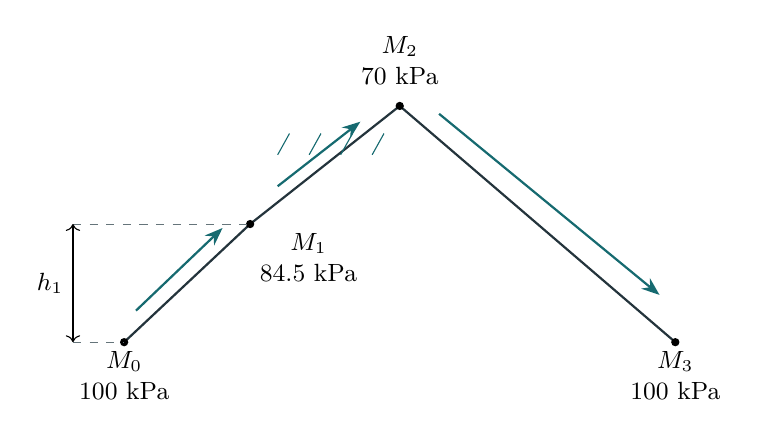
\begin{tikzpicture}[x=1cm,y=1cm]
\draw[object] (0,0)--(1.6,1.5)--(3.5,3)--(7,0);
\draw[motion] (.15,.4)--(1.25,1.45);
\draw[motion] (1.95,1.98)--(3,2.8);
\draw[motion] (4,2.9)--(6.8,.6);
\fill (0,0) circle(1.5pt) (1.6,1.5) circle(1.5pt) (3.5,3) circle(1.5pt) (7,0) circle(1.5pt);
\node[below,align=center] at (0,0) {$M_0$\\100 kPa};
\node[below right,align=center] at (1.6,1.5) {$M_1$\\84.5 kPa};
\node[above,align=center] at (3.5,3.15) {$M_2$\\70 kPa};
\node[below,align=center] at (7,0) {$M_3$\\100 kPa};
\draw[guide] (-.65,0)--(0,0) (-.65,1.5)--(1.6,1.5);
\draw[<->] (-.65,0)--(-.65,1.5) node[midway,left] {$h_1$};
\foreach \x in {2.1,2.5,2.9,3.3}{\draw[accent] (\x,2.65)--(\x-.15,2.38);}
\end{tikzpicture}\figcaption{图 热2.14　迎风侧成云降雨，背风侧按干绝热下沉估算。}\end{minipage}\end{center}

\Needspace{8\baselineskip}\subsection*{解答}

\textbf{按三段跟踪一份空气。}解图热2.14A把成云之前、凝结降雨、背风下降分别标出。比气体常量及压强指数为
\[r=c_p-c_V=c_p(1-1/\gamma),\qquad \kappa=(\gamma-1)/\gamma=2/7.\]
取$T_0=293.15\,\mathrm K$，将水汽对热容量和密度的影响忽略。
\begin{center}\begin{minipage}{0.96\linewidth}\centering
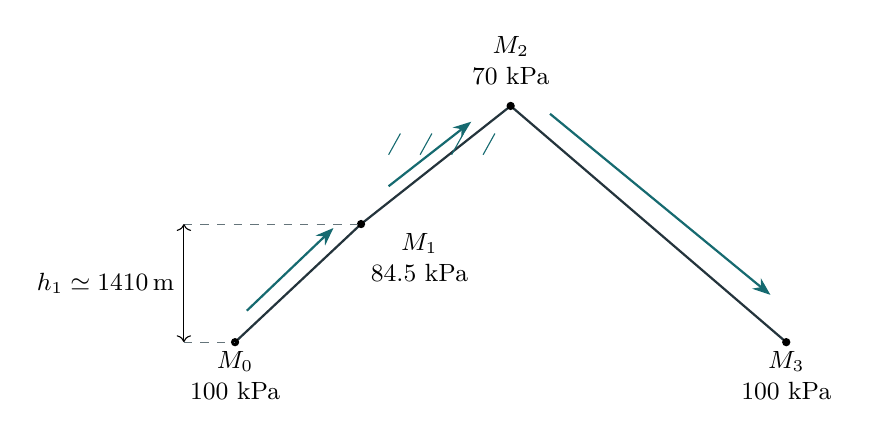
\begin{tikzpicture}[x=1cm,y=1cm]
\draw[object] (0,0)--(1.6,1.5)--(3.5,3)--(7,0);
\draw[motion] (.15,.4)--(1.25,1.45);
\draw[motion] (1.95,1.98)--(3,2.8);
\draw[motion] (4,2.9)--(6.8,.6);
\fill (0,0) circle(1.5pt) (1.6,1.5) circle(1.5pt) (3.5,3) circle(1.5pt) (7,0) circle(1.5pt);
\node[below,align=center] at (0,0) {$M_0$\\100 kPa};
\node[below right,align=center] at (1.6,1.5) {$M_1$\\84.5 kPa};
\node[above,align=center] at (3.5,3.15) {$M_2$\\70 kPa};
\node[below,align=center] at (7,0) {$M_3$\\100 kPa};
\draw[guide] (-.65,0)--(0,0) (-.65,1.5)--(1.6,1.5);
\draw[<->] (-.65,0)--(-.65,1.5) node[midway,left] {$h_1\simeq1410\,\mathrm m$};
\foreach \x in {2.1,2.5,2.9,3.3}{\draw[accent] (\x,2.65)--(\x-.15,2.38);}
\end{tikzpicture}\figcaption{解图 热2.14A　云底高度由迎风站到成云点的压强差和平均密度估算。}\end{minipage}\end{center}
\textbf{(1) 云底温度。}未凝结段采用干绝热关系$T/p^\kappa=\text{常量}$，故
\[T_1=T_0(p_1/p_0)^\kappa=293.15(84.5/100)^{2/7}
=279.3777\,\mathrm K\approx279\,\mathrm K.\]
\textbf{(2) 云底高度。}理想气体密度关系给出
\[\rho_1=\rho_0\frac{p_1T_0}{p_0T_1}=1.05423\,\mathrm{kg/m^3}.\]
密度线性下降时，空气柱平均密度$\bar\rho=(\rho_0+\rho_1)/2$。静压积分为
\[p_0-p_1=g\int_0^{h_1}\rho(h)\dd h
=\frac12g(\rho_0+\rho_1)h_1.\]
于是$h_1=1408.70\,\mathrm m$，按题给精度取$1410\,\mathrm m$。

\textbf{(3) 山顶温度的潜热估算。}先计算同样降压但不凝结时的温度
\[T_x=T_1(p_2/p_1)^\kappa=T_0(70/100)^{2/7}=264.7477\,\mathrm K.\]
每千克空气释放潜热$L_v m_c$，其中$m_c=0.00245\,\mathrm{kg/kg}$，相应等效增温
\[\Delta T=L_vm_c/c_p=6.09453\,\mathrm K.\]
所以估计$T_2=T_x+\Delta T=270.8422\,\mathrm K\approx271\,\mathrm K$。
\begin{center}\begin{minipage}{0.96\linewidth}\centering
\begin{tikzpicture}[x=1cm,y=1cm,font=\small]\node[draw,align=center] (a) at (0,0){$M_0$\\293 K};\node[draw,align=center] (b) at (2.8,0){$M_1$\\279 K};\node[draw,align=center] (c) at (5.8,0){$M_2$\\干绝热265 K\\潜热增温约6 K};\node[draw,align=center] (d) at (9,0){$M_3$\\300 K};\draw[motion] (a)--(b);\draw[motion] (b)--(c);\draw[motion] (c)--(d);
\end{tikzpicture}\figcaption{解图 热2.14B　潜热补偿部分绝热冷却；带着较高山顶温度下沉，使背风站更暖、更干。}\end{minipage}\end{center}
这里先求干绝热的降温，再把凝结放出的潜热折算为山顶处的温度补偿。凝结质量为原空气质量的0.245\%，质量变化按题设忽略。若逐步考虑潜热在后续上升中也被绝热冷却，其贡献为
\[\Delta T_2=\frac{L_v}{c_p}\int_{M_1}^{M_2}(p_2/p)^\kappa\,\dd m_c.\]
这里$\dd m_c$沿上升过程取正的凝结量。总凝结量固定时，$\Delta T_2$在$6.09453(70/84.5)^{2/7}$与$6.09453$之间，两端相差约0.32 K，小于题目1 K的分辨要求；具体温度轨迹随凝结量在各压强处的分配而改变。

\textbf{(4) 降雨量。}1500 s内每平方米的雨水质量为$2000\times0.00245=4.9\,\mathrm{kg/m^2}$。均匀持续3小时，
\[m_{\mathrm{rain}}=4.9\frac{3\times3600}{1500}=35.28\,\mathrm{kg/m^2}.\]
除以水密度$1000\,\mathrm{kg/m^3}$，得水深0.03528 m，取$35\,\mathrm{mm}$。

\textbf{(5) 背风温度。}降雨后下降段不再凝结，用干绝热压缩：
\[T_3=T_2(p_3/p_2)^\kappa=299.8984\,\mathrm K\approx300\,\mathrm K.\]
解图热2.14B沿空气越山路径比较温度：背风侧与迎风侧压强相同，温度较高、水汽含量较少。背风侧的下降增温提高了饱和水汽压，使相对湿度降低；经过凝结后剩余的水汽仍随气流到达背风侧。
\subsubsection*{研究对象、各段条件和近似的作用}
先取随气流越山的一份空气，按每千克初始空气计量，
把水汽凝结量$m_c$写成$\mathrm{kg/kg}$。
成云前$M_0\to M_1$尚无凝结，物质量在近似模型内固定，
可用干绝热的温压关系；云中$M_1\to M_2$仍对外绝热，
但水汽与空气之间因凝结发生内部能量传递，
潜热从凝结的水汽传给空气，属于气团内部的能量交换。
背风$M_2\to M_3$不再发生题设中的凝结降雨，
按相同的干绝热指数下降。下降时压强增加而温度升高，
下降段以实际山顶温度 $T_2$ 为起点。

题给每千克2.45 g对应$0.00245\,\mathrm{kg/kg}=0.245\%$，
这给出参与凝结的质量比例。水汽的热容量、密度贡献及少量质量流失已在题给模型中忽略，
汽化热也在相应温区内取常数。这样可把温度、状态与潜热关系保持为同一套常系数模型。
在上述常系数模型内，下一步用不同释放位置的权重给出山顶温度区间。

云底高度另使用了空气密度随高度线性变化的假设。
由成云前的温压关系，端点密度还可写成
\[
\rho_1=\rho_0(p_1/p_0)^{1/\gamma}.
\]
静力关系$\dd p=-\rho g\dd h$由$M_0$积分到$M_1$，
线性密度使积分恰等于梯形面积，
\[
\int_0^{h_1}\rho(h)\dd h
=\frac{\rho_0+\rho_1}{2}h_1.
\]
指定的线性密度使梯形面积精确给出这一模型的静压积分。
解图热2.14A的$h_1$竖标尺两端分别对齐山脚和云底，
标尺读出的是这两站之间的竖直高度差。

\subsubsection*{为什么潜热用定压热容量，以及释放时机的界限}
在每千克的理想气体模型内，设比容为$v$、比气体常量为$r$，
把凝结对空气部分的等效输入记为$\delta q=L_v\dd m_c$。
由第一定律及微分状态方程，
\[
c_V\dd T=\delta q-p\dd v,\qquad
p\dd v=r\dd T-rT\frac{\dd p}{p}.
\]
消去比容，得到
\[
c_p\dd T-rT\frac{\dd p}{p}=L_v\dd m_c,\qquad
\dd T-\kappa T\frac{\dd p}{p}=\frac{L_v}{c_p}\dd m_c.
\]
因此潜热项的温度系数为$L_v/c_p$，
其中的 $c_p=c_V+r$ 由内能项与膨胀功中的温度项相加得到。
$\dd m_c>0$沿上升过程表示已凝结的水增加，故潜热项为正，
它补偿降压造成的冷却。

对这一线性微分式乘积分因子$p^{-\kappa}$，在云底到山顶积分，
便得到前面的加权潜热式。越早放出的潜热，还会在随后降压中被冷却，
所以同样总凝结量在云底全部释放给最小贡献，山顶全部释放给最大贡献。
用本题数据，两个界限为
\[
5.775378\ \mathrm K\le\Delta T_2\le6.094527\ \mathrm K,
\]
\[
270.523078\ \mathrm K\le T_2\le270.842227\ \mathrm K.
\]
两端相差约0.31915 K，并且按本题取整都为271 K。
下降到100 kPa后，这个范围变成
\[
299.544964\ \mathrm K\le T_3\le299.898352\ \mathrm K,
\]
按1 K取整都为300 K。
两个端点都给出相同的整数温度，因此终态等效增温可用于本题要求的取整结果。
均匀雨强决定累计水深；求逐时温度时，还要给出沿途的压强和凝结量函数。

\subsubsection*{持续降雨的质量、面积与时间逐项换算}
降雨量是水平单位面积上累积雨水的水深。
一份处在降雨层的空气每平方米质量为2000 kg，
经历1500 s后相应凝结水为4.9 kg，所以均匀雨强为
\[
\dot m_{\rm rain}=\frac{4.9}{1500}
\,\mathrm{kg/(m^2\cdot s)}.
\]
将单位面积雨强乘3h对应的10800s，即得累计雨水质量。
累计35.28 $\mathrm{kg/m^2}$除以水密度，
\[
H=\frac{35.28\,\mathrm{kg/m^2}}{1000\,\mathrm{kg/m^3}}
=0.03528\,\mathrm m=35.28\,\mathrm{mm}.
\]
每平方米增加1 kg水就增加1 mm水深，取整后为35 mm。
水深由单位面积水质量除水密度得到，凝结比例和观测时长都线性进入这一结果。

$M_0$与$M_3$压强相同而温度不同：途中凝结释放潜热，随后下降继续压缩增温。
凝结降雨降低了空气的含水量，背风下降又降低相对湿度，
两种作用都使空气显得较干。
若另知剩余水汽分压和当地饱和水汽压，可用两者之比得到背风侧的相对湿度。
在采用同一比气体常量的近似内，同压较暖还意味着背风密度较低；
这一趋势与干暖的定性结论一致。


\Needspace{18\baselineskip}

\pdfbookmark[2]{第 15 题 U形管水银振动与封闭空气绝热弹性}{q15}

\section*{第 15 题\quad U形管水银振动与封闭空气绝热弹性}

等截面竖直U形管两端开口，管内水银全长$h$。压低一侧水银面，静止后撤去外压，忽略摩擦。证明振动周期$T_1=2\pi\sqrt{h/(2g)}$。再在两液面等高、气压等于大气压时封闭右端，封闭空气柱长$L$。气体作准静态绝热过程，水银作微小振动，证明
\[T_2=2\pi\sqrt{\frac{h}{g(2+\gamma h_0/L)}},\qquad \gamma=\frac{2L}{h_0}\left(\frac{T_1^2}{T_2^2}-1\right).\]
其中$h_0$为大气压对应的水银柱高度。

\begin{center}\begin{minipage}{0.96\linewidth}\centering
\begin{tikzpicture}[x=.9cm,y=.8cm]
\begin{scope}
\fill[accent!20] (0,0) rectangle (.7,1.8);
\fill[accent!20] (2.3,0) rectangle (3,1.2);
\fill[accent!20] (0,0) rectangle (3,.4);
\draw[object] (0,3.5)--(0,0)--(3,0)--(3,3.5);
\draw[object] (.7,3.5)--(.7,.4)--(2.3,.4)--(2.3,3.5);
\draw[guide] (-.4,1.5)--(3.4,1.5);
\draw[<->] (-.3,1.5)--(-.3,1.8) node[left,midway] {$y$};
\draw[<->] (3.35,1.2)--(3.35,1.5) node[right,midway] {$y$};
\node at (1.5,.2) {汞};
\node[above] at (.35,3.5) {$p_0$};
\node[above] at (2.65,3.5) {$p_0$};
\node[below] at (1.5,-.55) {两端开口};
\end{scope}
\begin{scope}[xshift=6.2cm]
\fill[accent!20] (0,0) rectangle (.7,1.8);
\fill[accent!20] (2.3,0) rectangle (3,1.2);
\fill[accent!20] (0,0) rectangle (3,.4);
\draw[object] (0,3.5)--(0,0)--(3,0)--(3,3.5);
\draw[object] (.7,3.5)--(.7,.4)--(2.3,.4)--(2.3,3.5);
\draw[guide] (-.4,1.5)--(3.4,1.5);
\draw[<->] (-.3,1.5)--(-.3,1.8) node[left,midway] {$y$};
\draw[<->] (3.35,1.2)--(3.35,1.5) node[right,midway] {$y$};
\node at (1.5,.2) {汞};
\draw[object] (2.3,3.5)--(3,3.5);
\draw[guide] (3,2.6)--(3.55,2.6);
\node[anchor=west,align=left] at (3.7,2.6) {封闭空气\\$L+y,\ p(y)$};
\node[above] at (.35,3.5) {$p_0$};
\node[below] at (1.5,-.55) {右端封闭};
\end{scope}
\end{tikzpicture}\figcaption{图 热2.15　以两液面等高的位置为$y=0$；左面升$y$时右面降$y$。}\end{minipage}\end{center}

\Needspace{8\baselineskip}\subsection*{解答}

\textbf{两端开口：整柱为惯性质量。}取左液面相对平衡面向上位移y，右面向下位移y，液面差$2y$；水银密度$\rho$，截面S。质量$m=\rho Sh$，全部水银的流速为$\dot y$。
\begin{center}\begin{minipage}{0.96\linewidth}\centering
\begin{tikzpicture}[x=.9cm,y=.8cm]
\begin{scope}
\fill[accent!20] (0,0) rectangle (.7,1.8);
\fill[accent!20] (2.3,0) rectangle (3,1.2);
\fill[accent!20] (0,0) rectangle (3,.4);
\draw[object] (0,3.5)--(0,0)--(3,0)--(3,3.5);
\draw[object] (.7,3.5)--(.7,.4)--(2.3,.4)--(2.3,3.5);
\draw[guide] (-.4,1.5)--(3.4,1.5);
\draw[<->] (-.3,1.5)--(-.3,1.8) node[left,midway] {$y$};
\draw[<->] (3.35,1.2)--(3.35,1.5) node[right,midway] {$y$};
\node at (1.5,.2) {汞};
\node[above] at (.35,3.5) {$p_0$};
\node[above] at (2.65,3.5) {$p_0$};
\node[below] at (1.5,-.55) {两端开口};
\end{scope}
\begin{scope}[xshift=6.2cm]
\fill[accent!20] (0,0) rectangle (.7,1.8);
\fill[accent!20] (2.3,0) rectangle (3,1.2);
\fill[accent!20] (0,0) rectangle (3,.4);
\draw[object] (0,3.5)--(0,0)--(3,0)--(3,3.5);
\draw[object] (.7,3.5)--(.7,.4)--(2.3,.4)--(2.3,3.5);
\draw[guide] (-.4,1.5)--(3.4,1.5);
\draw[<->] (-.3,1.5)--(-.3,1.8) node[left,midway] {$y$};
\draw[<->] (3.35,1.2)--(3.35,1.5) node[right,midway] {$y$};
\node at (1.5,.2) {汞};
\draw[object] (2.3,3.5)--(3,3.5);
\draw[guide] (3,2.6)--(3.55,2.6);
\node[anchor=west,align=left] at (3.7,2.6) {封闭空气\\$L+y,\ p(y)$};
\node[above] at (.35,3.5) {$p_0$};
\node[below] at (1.5,-.55) {右端封闭};
\end{scope}
\end{tikzpicture}\figcaption{解图 热2.15A　左图两端开口，右图封闭空气增加回复作用；同一坐标$y$决定液面差$2y$。}\end{minipage}\end{center}
解图热2.15A右图取左液面上移$y$、右液面下移$y$，封闭气柱长度便由$L$变成$L+y$，两液面的高度差改变$2y$。前一项进入气体压强的变化，后一项进入重力恢复压差。解图热2.15B中封闭气体对应的势能曲线更陡，正是附加气体刚度使周期缩短的图像。

高度转移的水银质量$\rho Sy$，其重心平均提升y，故势能增加$\rho Sgy^2$。由初始静止振幅$a$时的机械能守恒
\[\tfrac12\rho Sh\dot y^2+\rho Sgy^2=\rho Sga^2.\]
微分或直接写回复力$-2\rho Sgy$，均得
\[\ddot y+\frac{2g}{h}y=0,\qquad
T_1=2\pi\sqrt{\frac{h}{2g}}.\]
\textbf{封闭右端：空气再提供回复力。}封闭前两面等高，故平衡气压$p_0=\rho gh_0$。左面上升y时右面下降，气柱长$L+y$，绝热关系为
\[p(y)[S(L+y)]^\gamma=p_0(SL)^\gamma.\]
在$|y|\ll L$下
\[p(y)-p_0=p_0[(1+y/L)^{-\gamma}-1]
=-\gamma p_0y/L+p_0O(y^2/L^2).\]
左侧大气作用的广义力为$-p_0S$，右侧气体为$p(y)S$，故合压力为$[p(y)-p_0]S$。加上重力回复项，
\[\rho Sh\ddot y=-2\rho Sgy+[p(y)-p_0]S.\]
线性化即
\[\ddot y+\frac{g}{h}(2+\gamma h_0/L)y=0.\]
\begin{center}\begin{minipage}{0.96\linewidth}\centering
\begin{tikzpicture}[x=1cm,y=1cm]
\draw[axis] (-2.5,0)--(2.8,0) node[right] {$y$};
\draw[axis] (0,0)--(0,4.5) node[above] {$E_{\rm pot}$};
\draw[traj,domain=-2:2,samples=70] plot (\x,{.6*\x*\x});
\draw[warm,thick,domain=-2:2,samples=70] plot (\x,{.95*\x*\x});
\node[below left] at (0,0) {$0$};
\node[right] at (2.1,2.4) {两端开口};
\node[right] at (2.1,3.8) {右端封闭};
\end{tikzpicture}\figcaption{解图 热2.15B　以平衡位置势能为零；封闭空气增加弹性系数，使周期减小。}\end{minipage}\end{center}
\result{T_2=2\pi\sqrt{\frac{h}{g(2+\gamma h_0/L)}}.}
水银的机械能变化也可由两侧压强所作的功给出，$\dd E_{\mathrm{Hg}}=[p(y)-p_0]S\dd y$。从释放点 $a$ 算起，积分下限为 $a$。在线性近似下，将空气回复作用移入势能，得到
\[\tfrac12\rho Sh\dot y^2+
\tfrac12\rho Sg(2+\gamma h_0/L)y^2=\text{常量},\]
与动力学式相符。单独水银的机械能不守恒，气体与恒压大气作用合成的有效势能加入后，才有上述守恒量。

两周期相除，
\[T_1^2/T_2^2=1+\gamma h_0/(2L),\]
\result{\gamma=\frac{2L}{h_0}(T_1^2/T_2^2-1).}
$T_2<T_1$、$L\to\infty$时$T_2\to T_1$。若封闭后的平衡液面有高度差，记实际平衡压强、气柱长度为 $p_e,L_e$，由局部绝热压强斜率得气体刚度 $\gamma p_eS/L_e$。
\subsubsection*{重力势能与整柱惯性的两个系数}
解图热2.15A左图取两液面初始共同高度为零。
左面升$y$、右面降$y$时，相当于把右臂$[-y,0]$的一段水银移到左臂$[0,y]$。
转移质量为$\Delta m=\rho Sy$，两段重心分别在$-y/2$与$y/2$，
所以重心升高为$y$，重力势能增加为$\rho Sgy^2$。
转移水银的重心抬升 $y$，液面高度差 $2y$ 则进入静压差。
全部水银沿等截面管流动，各截面流速大小相同，
各处共同的流速使整柱质量 $\rho Sh$ 都进入动能。

开口情形能量写成
\[
gy^2+\frac h2\dot y^2=ga^2.
\]
对时间求导得到
\[
2gy\dot y+h\dot y\ddot y=0.
\]
在$\dot y\ne0$区间约去$\dot y$得到简谐方程，
转折点的加速度可由连续性延拓，也可直接用
$\rho Sh\ddot y=-2\rho Sgy$，该运动方程也给出转折点的加速度。
两端均为$p_0$时压力功相互抵消，水银与地球的机械能确实守恒。
只要两液面仍在等截面竖直臂内，这一开口模型的重力项就是线性的；
封闭气体那一部分才另要求$|y|/L$很小。

\subsubsection*{封闭气体的压力功与有效位移势能}
解图热2.15A右图中，$y>0$使气柱增长、气压降低。
右气体对水银的功微元为$p(y)S\dd y$，
左大气作用为$-p_0S\dd y$，合为$[p(y)-p_0]S\dd y$。
若水银从静止释放点$a$运动到$y$，
正确的功能关系为
\[
E_{\rm Hg}(y,\dot y)-E_{\rm Hg}(a,0)
=S\int_a^y[p(u)-p_0]\dd u.
\]
从释放点积分时，常数取释放点的机械能；从平衡点积分则以平衡点为势能零点。

也可将气体和恒压大气的作用一起写成有效位移势能。
对$\gamma\ne1$，令其在$y=0$为零，得
\[
\Phi_p(y)=-S\int_0^y[p(u)-p_0]\dd u
=p_0Sy+\frac{p_0SL}{\gamma-1}
[(1+y/L)^{1-\gamma}-1].
\]
其中第二项是绝热气体的内能变化，第一项是恒压大气作用对应的势能。取 $\gamma=1$ 的对数积分时，$\Phi_p=p_0S[y-L\ln(1+y/L)]$。
因此完整的守恒式为
\[
\frac12\rho Sh\dot y^2+\rho Sgy^2+\Phi_p(y)=E.
\]
其中 $p_0Sy$ 是左端恒定大气压力对应的势能项。

在$|y|\ll L$时，
\[
\Phi_p(y)=\frac{\gamma p_0S}{2L}y^2
-\frac{\gamma(\gamma+1)p_0S}{6L^2}y^3+O(y^4).
\]
保留二次势能后，重力刚度$k_g=2\rho Sg$，
气体刚度$k_{\rm gas}=\gamma p_0S/L$，
所以$\omega_2^2=(k_g+k_{\rm gas})/(\rho Sh)$，
与前述动力学线性化一致。解图热2.15B的两条抛物线只表示这一小振动范围；
大振幅时三次等高阶项会使势能不再关于$y=0$对称，周期也可能依赖振幅。

将 $p_0=\rho gh_0$ 代入，得
$g(2+\gamma h_0/L)/h$，括号里的两项均无量纲。
反求式同样只含长度比与周期比，量纲为纯数。
当气柱极长时附加刚度趋零，$T_2\to T_1$；
理想封闭气柱的附加刚度为正，因而 $T_2<T_1$。实测若得到 $T_2\ge T_1$，可分别测定封口漏气、振幅衰减与周期读数误差，再按对应的振动模型求 $\gamma$。


\Needspace{18\baselineskip}

\pdfbookmark[2]{第 16 题 由声速驻波判断碘蒸气分子类型}{q16}

\section*{第 16 题\quad 由声速驻波判断碘蒸气分子类型}

在$400\,\mathrm K$的碘蒸气管中，用$1000\,\mathrm{Hz}$声波形成驻波，相邻波节间距6.77 cm。碘原子相对原子质量127。按理想气体模型判断蒸气分子是单原子还是双原子。给定声速$v=1/\sqrt{\rho K_s}$，其中$K_s=-V^{-1}(\dd V/\dd p)_{\mathrm{ad}}$为绝热压缩系数。

\begin{center}\begin{minipage}{0.96\linewidth}\centering
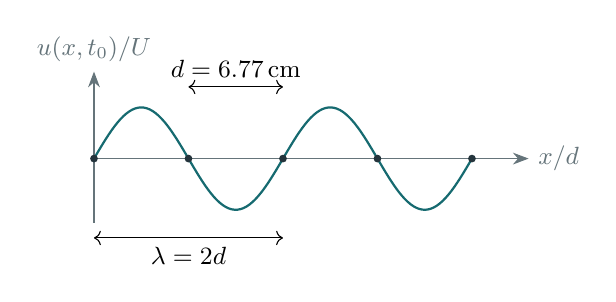
\begin{tikzpicture}[x=1.2cm,y=.65cm]
\draw[axis] (0,0)--(4.6,0) node[right] {$x/d$};
\draw[axis] (0,-1.25)--(0,1.7) node[above] {$u(x,t_0)/U$};
\draw[traj,domain=0:4,samples=130] plot (\x,{sin(180*\x)});
\foreach \x in {0,1,2,3,4}{\fill[ink] (\x,0) circle(1.4pt);}
\draw[<->] (1,1.4)--(2,1.4) node[midway,above] {$d=6.77\,\mathrm{cm}$};
\draw[<->] (0,-1.55)--(2,-1.55) node[midway,below] {$\lambda=2d$};
\end{tikzpicture}\figcaption{图 热2.16　相邻波节间距为半波长；曲线表示固定时刻的位移。}\end{minipage}\end{center}

\Needspace{8\baselineskip}\subsection*{解答}

\textbf{从绝热压缩系数导出声速。}理想气体准静态绝热满足$pV^\gamma=\text{常量}$，微分得到
\[V^\gamma\dd p+\gamma pV^{\gamma-1}\dd V=0,\qquad
(\dd V/\dd p)_{\mathrm{ad}}=-V/(\gamma p).\]
所以$K_s=1/(\gamma p)$。又由$pV=MRT/\mu$，$\rho=M/V=p\mu/(RT)$。代入题给声速式：
\[v^2=\frac{1}{\rho K_s}=\frac{\gamma RT}{\mu},\qquad
\gamma=\frac{\mu v^2}{RT}.\]
\begin{center}\begin{minipage}{0.96\linewidth}\centering
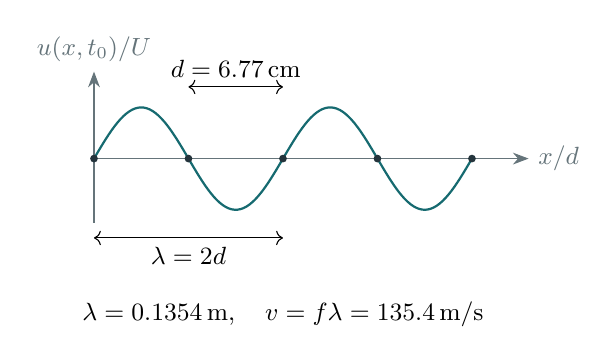
\begin{tikzpicture}[x=1.2cm,y=.65cm]
\draw[axis] (0,0)--(4.6,0) node[right] {$x/d$};
\draw[axis] (0,-1.25)--(0,1.7) node[above] {$u(x,t_0)/U$};
\draw[traj,domain=0:4,samples=130] plot (\x,{sin(180*\x)});
\foreach \x in {0,1,2,3,4}{\fill[ink] (\x,0) circle(1.4pt);}
\draw[<->] (1,1.4)--(2,1.4) node[midway,above] {$d=6.77\,\mathrm{cm}$};
\draw[<->] (0,-1.55)--(2,-1.55) node[midway,below] {$\lambda=2d$};
\node[below,align=center] at (2,-2.6)
 {$\lambda=0.1354\,\mathrm m,\quad v=f\lambda=135.4\,\mathrm{m/s}$};
\end{tikzpicture}\figcaption{解图 热2.16A　由波节间距求波长和声速，再用两种候选摩尔质量分别求绝热指数。}\end{minipage}\end{center}
解图热2.16A中相邻驻波节点间距$d$对应半个波长，故先用$\lambda=2d$求声速，再由$v^2=\gamma RT/\mu$反推$\gamma$。把碘原子和双原子分子各自的摩尔质量代入声速式，得到两组 $\gamma$，再分别与该分子模型的热容量比比较。

\textbf{驻波读数给波长。}相邻两节的空间相位差为 $\pi$，故 $d=\lambda/2$，于是
\[\lambda=2d=0.1354\,\mathrm m,\qquad
v=f\lambda=135.4\,\mathrm{m/s}.\]
两种候选分别代入$T=400\,\mathrm K$、$R=8.314$：
\[\begin{array}{c|c|c|c}
\text{候选} & \mu/(\mathrm{kg/mol}) & \gamma\text{的实验值} & \text{模型值}\\\hline
\mathrm I & 0.127 & 0.70012 & 5/3\\
\mathrm I_2 & 0.254 & 1.40024 & 7/5
\end{array}\]
在题设理想气体、双原子转动充分激发且振动贡献忽略的模型下，双原子候选与观测相符：
\result{\text{碘蒸气分子为}\ \mathrm I_2.}
单原子候选给出小于1的指数，与理想气体模型不相容；双原子判断以本题给定的温区与自由度近似为条件。
\subsubsection*{由压缩性到声速的完整量纲链}
气体中的小幅纵向声波需要体积弹性，给定的$K_s$是绝热压缩系数，
其量纲为$\mathrm{Pa^{-1}}$。
从$pV^\gamma$不变得
\[
\frac{\dd p}{p}+\gamma\frac{\dd V}{V}=0,\qquad
K_s=-\frac1V\left(-\frac V{\gamma p}\right)=\frac1{\gamma p}>0.
\]
再用$\rho=p\mu/(RT)$，有
\[
\rho K_s=\frac{\mu}{\gamma RT},
\qquad
\frac1{\rho K_s}=\frac{\gamma RT}{\mu}.
\]
压强消去，因此在理想气体、相同$T,\mu,\gamma$的模型内，
改变压强本身不改变声速。
摩尔质量与 SI 制的 $R$ 配套，I 的 $127\,\mathrm{g/mol}$ 换成 $0.127\,\mathrm{kg/mol}$。

解图热2.16A以$x/d$为横坐标，相邻位移波节相距一个$d$，
相邻两个波腹振动反相，隔一个波腹才同相。两个同相波腹之间的距离是一个完整波长 $2d$。
因此用$6.77$ cm得到13.54 cm的波长，再换成0.1354 m，
与1000 Hz相乘给135.4 m/s。
相邻同类节点给出同一个半波长。两种候选都使用由这个节距求得的声速，只改变所代入的摩尔质量。

\begin{center}\begin{minipage}{0.96\linewidth}\centering
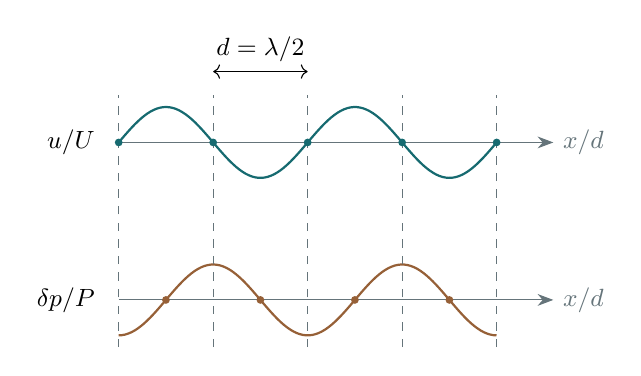
\begin{tikzpicture}[x=1.2cm,y=1cm]
\draw[axis] (0,2)--(4.6,2) node[right] {$x/d$};
\draw[axis] (0,0)--(4.6,0) node[right] {$x/d$};
\draw[traj,domain=0:4,samples=120] plot (\x,{2+.45*sin(180*\x)});
\draw[warm,thick,domain=0:4,samples=120] plot (\x,{-.45*cos(180*\x)});
\foreach \x in {0,1,2,3,4}{
 \draw[guide] (\x,-.6)--(\x,2.6);
 \fill[accent] (\x,2) circle(1.4pt);
}
\foreach \x in {.5,1.5,2.5,3.5}{\fill[warm] (\x,0) circle(1.4pt);}
\node[left] at (-.15,2) {$u/U$};
\node[left] at (-.15,0) {$\delta p/P$};
\draw[<->] (1,2.9)--(2,2.9) node[midway,above] {$d=\lambda/2$};
\end{tikzpicture}
\figcaption{解图 热2.16B　同一时刻的位移与压强扰动；位移节对应压强腹，同类相邻节距均为$\lambda/2$。}
\end{minipage}\end{center}
图中$U$为位移振幅，$P=\gamma pkU$为压强扰动振幅，$k=2\pi/\lambda$；所选时刻满足$\cos\omega t_0=1$。
若取位移$u=U\sin(kx)\cos\omega t$，
压强扰动为
\[
\delta p=-\frac1{K_s}\frac{\partial u}{\partial x}
=-\gamma p\,kU\cos(kx)\cos\omega t.
\]
所以位移的节与压强的节相差四分之一波长，
两列节点分开读数，各取相邻两个同类节点量半波长。

\subsubsection*{由两种候选分子的声速与节距确定分子类型}
将两种候选分子的摩尔质量和绝热指数分别代入声速式，可直接求出各自的驻波节距。
单原子I若取$\mu=0.127$、$\gamma=5/3$，
\[
v_{\rm I}\simeq208.909\,\mathrm{m/s},\qquad
d_{\rm I}=v_{\rm I}/(2f)\simeq10.4455\,\mathrm{cm},
\]
明显偏离实测6.77 cm。
双原子I$_2$若取$\mu=0.254$、$\gamma=7/5$，
\[
v_{\rm I_2}\simeq135.389\,\mathrm{m/s},\qquad
d_{\rm I_2}\simeq6.76943\,\mathrm{cm},
\]
与实测相符。这里由候选分子的摩尔质量与热容量预测声速，再用相邻波节相距半个波长的关系得到节距。

理想气体有$C_p-C_V=R$和正的$C_V$，
因此$\gamma=1+R/C_V>1$。单原子候选用本模型算出的约0.70既低于1，
也不等于单原子自由度所需的$5/3$。
本题按理想气体声速关系比较I与I$_2$两种候选。在实验温度下，I$_2$采用平动和转动自由度对应的热容量，$C_V=5R/2$、$C_p=7R/2$，给出$\gamma=7/5$。这一候选的摩尔质量、热容量与观测节距共同确定了上述判断。


\Needspace{18\baselineskip}

\pdfbookmark[2]{第 17 题 两个三角循环效率的比较}{q17}

\section*{第 17 题\quad 两个三角循环效率的比较}

定容摩尔热容量$C_V$恒定的理想气体经历图示两个顺时针三角循环$A_iB_iC_iA_i$（$i=1,2$）。两循环共用体积端点$V_1,V_2$；$A_iB_i$为过原点的直线$p=k_iV$，$B_iC_i$等容降压，$C_iA_i$等压压缩。比较效率$\eta_1,\eta_2$。

\begin{center}\begin{minipage}{0.96\linewidth}\centering
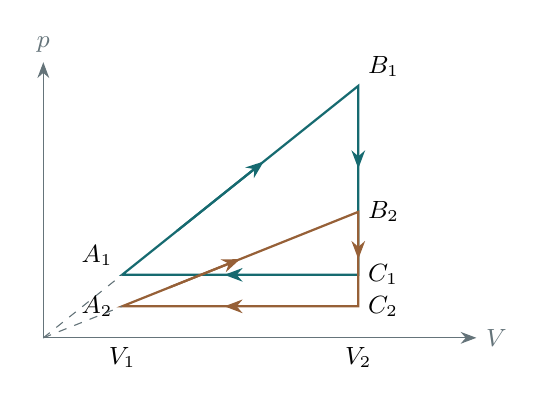
\begin{tikzpicture}[x=1cm,y=1cm,font=\small]\draw[axis] (0,0)--(5.5,0) node[right] {$V$};\draw[axis] (0,0)--(0,3.5) node[above] {$p$};
\draw[traj] (1,.8)--(4,3.2)--(4,.8)--cycle;\draw[warm,thick] (1,.4)--(4,1.6)--(4,.4)--cycle;\draw[guide] (0,0)--(1,.8);\draw[guide] (0,0)--(1,.4);\node[below] at (1,0){$V_1$};\node[below] at (4,0){$V_2$};\node[above left] at (1,.8){$A_1$};\node[above right] at (4,3.2){$B_1$};\node[right] at (4,.8){$C_1$};\node[left] at (1,.4){$A_2$};\node[right] at (4,1.6){$B_2$};\node[right] at (4,.4){$C_2$};
\draw[motion] (1.7,1.36)--(2.8,2.24);
\draw[motion] (4,2.8)--(4,2.15);
\draw[motion] (3.2,.8)--(2.3,.8);
\draw[motion,color=warm] (1.6,.64)--(2.5,1);
\draw[motion,color=warm] (4,1.4)--(4,1);
\draw[motion,color=warm] (3.2,.4)--(2.3,.4);
\end{tikzpicture}\figcaption{图 热2.17　同一体积端点下，两循环的压力尺度不同。}\end{minipage}\end{center}

\Needspace{8\baselineskip}\subsection*{解答}

\textbf{先确定吸热所在的边。}对任意一个循环，记射线斜率k。AB膨胀且$p=kV$，温度从$kV_1^2/(\nu R)$升至$kV_2^2/(\nu R)$。BC等容降温，$Q_{BC}<0$；CA等压压缩降温，$Q_{CA}<0$。所以效率的分母只取 AB 的正热量，循环的净热量等于有向面积表示的净功。
\begin{center}\begin{minipage}{0.96\linewidth}\centering
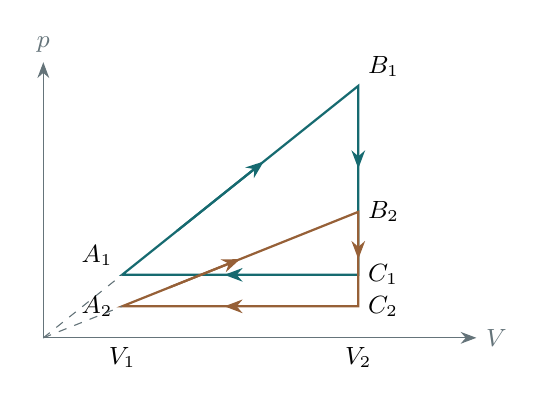
\begin{tikzpicture}[x=1cm,y=1cm,font=\small]\draw[axis] (0,0)--(5.5,0) node[right] {$V$};\draw[axis] (0,0)--(0,3.5) node[above] {$p$};
\draw[traj] (1,.8)--(4,3.2)--(4,.8)--cycle;\draw[warm,thick] (1,.4)--(4,1.6)--(4,.4)--cycle;\draw[guide] (0,0)--(1,.8);\draw[guide] (0,0)--(1,.4);\node[below] at (1,0){$V_1$};\node[below] at (4,0){$V_2$};\node[above left] at (1,.8){$A_1$};\node[above right] at (4,3.2){$B_1$};\node[right] at (4,.8){$C_1$};\node[left] at (1,.4){$A_2$};\node[right] at (4,1.6){$B_2$};\node[right] at (4,.4){$C_2$};\draw[motion] (1.7,1.36)--(2.8,2.24);\draw[motion] (4,2.8)--(4,2.15);\draw[motion] (3.2,.8)--(2.3,.8);
\draw[motion,color=warm] (1.6,.64)--(2.5,1);
\draw[motion,color=warm] (4,1.4)--(4,1);
\draw[motion,color=warm] (3.2,.4)--(2.3,.4);
\end{tikzpicture}\figcaption{解图 热2.17A　每个循环只有$A_iB_i$吸热；压力尺度$k_i$在功与吸热量中同比出现。}\end{minipage}\end{center}
解图热2.17A中，同体积端点的每个三角循环只有$A_iB_i$段吸热，$B_iC_i$及$C_iA_i$段均放热。把吸热积分限制在$A_iB_i$上，分母才是正吸热总量；分子则取图中整个三角形的有向面积。压强按同一倍数改变，使功与吸热按同一比例变化，所以相应效率相同。

AB上$\nu R\dd T=\dd(pV)=2kV\dd V$，第一定律给出
\[\delta Q=\nu C_V\dd T+kV\dd V
=\nu(C_V+R/2)\dd T.\]
其过程摩尔热容量为
\[C=C_V+R/2=\frac{\gamma+1}{2}C_V,\]
等价于多方指数$n=-1$。因此
\[Q_{\mathrm{in}}=\frac{kC}{R}(V_2^2-V_1^2).\]
三角形有向面积是净功：
\[W=\tfrac12[kV_2-kV_1](V_2-V_1)=\tfrac12k(V_2-V_1)^2.\]
\Needspace{11\baselineskip}
相除得
\[\eta=\frac{R(V_2-V_1)}{2C(V_2+V_1)}
=\frac{\gamma-1}{\gamma+1}\frac{V_2-V_1}{V_2+V_1}.\]
k同时乘在功和吸热中，完全消去。两个循环同一气体且体积端点相同，故
\result{\eta_1=\eta_2.}
较陡射线可有更大的功和更大的工作温区，效率仍相同；若改体积比或热容量，这个结论不再自动成立。
\subsubsection*{三角循环各段的温度、热量和净功}
以解图热2.17A中的任一循环为对象，
\[
T_A=\frac{kV_1^2}{\nu R},\qquad
T_B=\frac{kV_2^2}{\nu R},\qquad
T_C=\frac{kV_1V_2}{\nu R}.
\]
由$0<V_1<V_2$，有$T_A<T_C<T_B$。
沿$A\to B$升温膨胀，功和热均为正；
$B\to C$定容降温只放热，$C\to A$定压压缩也放热。
将每一项都写出来，令$\Delta V=V_2-V_1>0$：
\[
\begin{aligned}
Q_{AB}&=\frac{k(C_V+R/2)}R\Delta V(V_2+V_1)>0,\\
Q_{BC}&=-\frac{kC_V}R\,V_2\Delta V<0,\\
Q_{CA}&=-\frac{kC_p}R\,V_1\Delta V<0.
\end{aligned}
\]
其中第二项用了$T_C-T_B=-kV_2\Delta V/(\nu R)$，
第三项用了$T_A-T_C=-kV_1\Delta V/(\nu R)$。
因此正吸热总量为$Q_{\rm in}=Q_{AB}$，
放热绝对值为
\[
Q_{\rm out}=\frac{k\Delta V}R(C_VV_2+C_pV_1).
\]
用$C_p=C_V+R$相减得到
\[
Q_{\rm in}-Q_{\rm out}=\frac{k}{2}(\Delta V)^2=W,
\]
这就是图中三角形的有向面积。效率的分母为$A\to B$段从热源吸收的热量，分子为整个循环输出的净功。

射线$p=kV$还可按多方过程写成$pV^{-1}=k$，
沿射线直接对状态方程求微分，
$\nu R\dd T=2kV\dd V$直接给$\delta Q/\dd T=\nu(C_V+R/2)$。
于是$C=(\gamma+1)C_V/2$，它由气体热容量决定，与射线斜率$k$无关。

\subsubsection*{压力成比例变化时的效率}
若$k_1=a k_2$，两循环相同体积处的压力、所有端点温度、
各边热量及净功都乘$a$，所以效率保持不变。
在图上，每个体积处的压强同比变化，两个三角形沿纵轴成比例伸缩。
温度范围也随压力伸缩。若热容量随温度而变，分别沿两条吸热边对 $C_V(T)+R/2$ 积分。

令$q=V_2/V_1>1$，结果写成
\[
\eta=\frac{\gamma-1}{\gamma+1}\frac{q-1}{q+1},
\qquad
\frac{\dd\eta}{\dd q}
=\frac{2(\gamma-1)}{(\gamma+1)(q+1)^2}>0.
\]
$q\to1$时，净功为体积差的二阶量，吸热为一阶量，
故效率趋零；$q\to\infty$时，趋向$(\gamma-1)/(\gamma+1)$。
同一种气体采用不同体积比时，体积比大的循环效率较高。
取单原子气体与体积比 $q=2$，有 $C=2R$，
$W=kV_1^2/2,Q_{\rm in}=6kV_1^2$，效率为$1/12$；
双原子相同几何则为$1/18$。


\Needspace{18\baselineskip}

\pdfbookmark[2]{第 18 题 多条过程线构成循环的效率比较}{q18}

\section*{第 18 题\quad 多条过程线构成循环的效率比较}

理想气体的$C_V$为常量。图中两曲线为不同绝热线，三条直线的延长线过原点：12在$p=k_3V$上，34在$p=k_2V$上，56在$p=k_1V$上，$k_3>k_2>k_1>0$。1、3、5在同一绝热线上，2、4、6在另一线上。比较$\eta_{12431}$与$\eta_{12651}$；当三射线在同一参考体积处的压强比$p_1^*:p_2^*:p_3^*=1:2:3$时，再比较$\eta_{12431}$与$\eta_{34653}$。

\begin{center}\begin{minipage}{0.96\linewidth}\centering
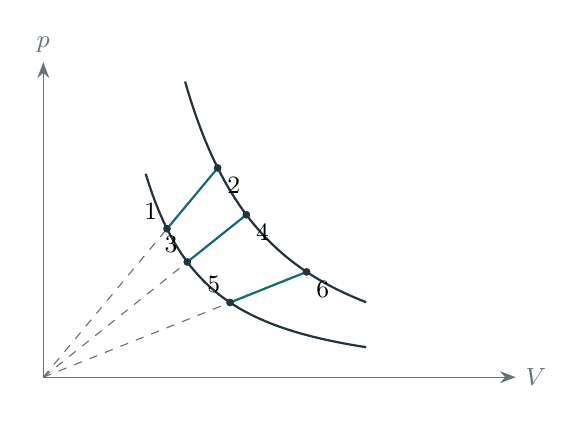
\begin{tikzpicture}[x=1cm,y=1cm,font=\small]\draw[axis] (0,0)--(6,0) node[right] {$V$};\draw[axis] (0,0)--(0,4) node[above] {$p$};
\draw[ink,thick,domain=1.3:4.1,samples=65] plot (\x,{4/pow(\x,5/3)});
\draw[ink,thick,domain=1.8:4.1,samples=65] plot (\x,{10/pow(\x,5/3)});
\draw[guide] (0,0)--(1.5706504008343012,1.8847804810011612);\draw[traj] (1.5706504008343012,1.8847804810011612)--(2.2146598521303114,2.6575918225563737);\fill[ink] (1.5706504008343012,1.8847804810011612) circle(1.4pt);\node[above left] at (1.5706504008343012,1.8847804810011612) {1};
\fill[ink] (2.2146598521303114,2.6575918225563737) circle(1.4pt);\node[below right] at (2.2146598521303114,2.6575918225563737) {2};
\draw[guide] (0,0)--(1.8285790999795744,1.4628632799836596);\draw[traj] (1.8285790999795744,1.4628632799836596)--(2.5783463443031147,2.0626770754424917);\fill[ink] (1.8285790999795744,1.4628632799836596) circle(1.4pt);\node[above left] at (1.8285790999795744,1.4628632799836596) {3};
\fill[ink] (2.5783463443031147,2.0626770754424917) circle(1.4pt);\node[below right] at (2.5783463443031147,2.0626770754424917) {4};
\draw[guide] (0,0)--(2.371373705661655,0.9485494822646621);\draw[traj] (2.371373705661655,0.9485494822646621)--(3.34370152488211,1.337480609952844);\fill[ink] (2.371373705661655,0.9485494822646621) circle(1.4pt);\node[above left] at (2.371373705661655,0.9485494822646621) {5};
\fill[ink] (3.34370152488211,1.337480609952844) circle(1.4pt);\node[below right] at (3.34370152488211,1.337480609952844) {6};

\end{tikzpicture}\figcaption{图 热2.18　两条绝热线与三条过原点射线相交；点号按循环路径排列。}\end{minipage}\end{center}

\Needspace{8\baselineskip}\subsection*{解答}

\textbf{把三段射线的吸热独立记号。}沿12、34、56由内绝热线到外绝热线都是膨胀升温；其多方指数均$n=-1$，过程摩尔热容量同为$C=C_V+R/2$。分别记正吸热$Q_h,Q_m,Q_l$，其反向过程各放出同量热。两条绝热边不交换热量。
\begin{center}\begin{minipage}{0.96\linewidth}\centering
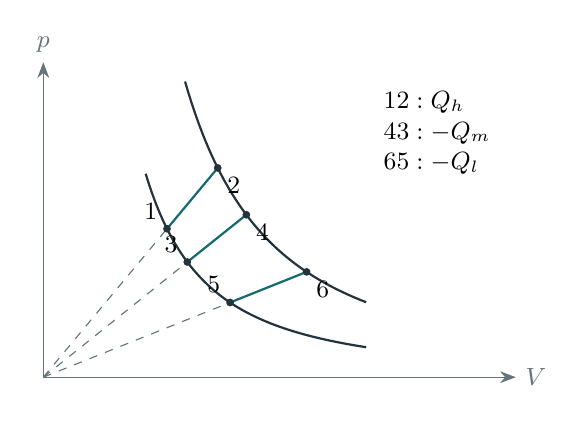
\begin{tikzpicture}[x=1cm,y=1cm,font=\small]\draw[axis] (0,0)--(6,0) node[right] {$V$};\draw[axis] (0,0)--(0,4) node[above] {$p$};
\draw[ink,thick,domain=1.3:4.1,samples=65] plot (\x,{4/pow(\x,5/3)});
\draw[ink,thick,domain=1.8:4.1,samples=65] plot (\x,{10/pow(\x,5/3)});
\draw[guide] (0,0)--(1.5706504008343012,1.8847804810011612);\draw[traj] (1.5706504008343012,1.8847804810011612)--(2.2146598521303114,2.6575918225563737);\fill[ink] (1.5706504008343012,1.8847804810011612) circle(1.4pt);\node[above left] at (1.5706504008343012,1.8847804810011612) {1};
\fill[ink] (2.2146598521303114,2.6575918225563737) circle(1.4pt);\node[below right] at (2.2146598521303114,2.6575918225563737) {2};
\draw[guide] (0,0)--(1.8285790999795744,1.4628632799836596);\draw[traj] (1.8285790999795744,1.4628632799836596)--(2.5783463443031147,2.0626770754424917);\fill[ink] (1.8285790999795744,1.4628632799836596) circle(1.4pt);\node[above left] at (1.8285790999795744,1.4628632799836596) {3};
\fill[ink] (2.5783463443031147,2.0626770754424917) circle(1.4pt);\node[below right] at (2.5783463443031147,2.0626770754424917) {4};
\draw[guide] (0,0)--(2.371373705661655,0.9485494822646621);\draw[traj] (2.371373705661655,0.9485494822646621)--(3.34370152488211,1.337480609952844);\fill[ink] (2.371373705661655,0.9485494822646621) circle(1.4pt);\node[above left] at (2.371373705661655,0.9485494822646621) {5};
\fill[ink] (3.34370152488211,1.337480609952844) circle(1.4pt);\node[below right] at (3.34370152488211,1.337480609952844) {6};
\node[align=left] at (5,3.1){$12:Q_h$\\$43: -Q_m$\\$65: -Q_l$};
\end{tikzpicture}\figcaption{解图 热2.18A　两循环共用吸热段12，较低射线提供较少的放热。}\end{minipage}\end{center}
解图热2.18A的三条斜射线分别对应$p=kV$，两条边界曲线是绝热支。把相邻两个小循环拼合时，中间射线上的热量以相反方向出现并相消，外圈留下最高射线吸热、最低射线放热。这一图中路径的拼合关系决定后面的热量比例，效率合并须按中间热量占比加权。

三个顺时针循环的效率于是为
\[\eta_{12431}=1-Q_m/Q_h,\qquad
\eta_{12651}=1-Q_l/Q_h,\qquad
\eta_{34653}=1-Q_l/Q_m.\]
\textbf{确定热量怎样随射线斜率变。}设两绝热线常量为$a<b$，射线$p=kV$的两个交点满足
\[kV_a^{\gamma+1}=a,\qquad kV_b^{\gamma+1}=b.\]
故体积比$V_b/V_a=(b/a)^{1/(\gamma+1)}=\alpha$，与k无关。该射线的吸热
\[Q(k)=\frac{kC}{R}(V_b^2-V_a^2)
=\frac{C}{R}(\alpha^2-1)a^{2/(\gamma+1)}k^{(\gamma-1)/(\gamma+1)}.\]
令$\beta=(\gamma-1)/(\gamma+1)>0$，则
\[Q_h:Q_m:Q_l=k_3^\beta:k_2^\beta:k_1^\beta.\]
由$k_3>k_2>k_1$直接知$Q_h>Q_m>Q_l$，所以
\result{\eta_{12431}<\eta_{12651}.}
\Needspace{11\baselineskip}
此比较不需要具体压强比。第二问在同一参考体积读压强，故$k_1:k_2:k_3=1:2:3$，从而
\[\eta_{12431}=1-(2/3)^\beta,\qquad
\eta_{34653}=1-(1/2)^\beta.\]
因$(2/3)^\beta>(1/2)^\beta$，
\result{\eta_{12431}<\eta_{34653}.}
两个相邻循环各自用高射线的吸热作分母，因此比较的是吸、放热之比。
\subsubsection*{六个交点的温度差逐步写出}
解图热2.18A中，内绝热线为$pV^\gamma=a$，外线为$pV^\gamma=b$，
且$b>a>0$。射线$p=kV$与二者交于
\[
V_a(k)=a^{1/(\gamma+1)}k^{-1/(\gamma+1)},\qquad
V_b(k)=b^{1/(\gamma+1)}k^{-1/(\gamma+1)}.
\]
所以三个体积比分别满足
\[
\frac{V_2}{V_1}=\frac{V_4}{V_3}=\frac{V_6}{V_5}
=(b/a)^{1/(\gamma+1)}=\alpha>1.
\]
在同一射线上，温度为$T=kV^2/(\nu R)$，进一步得
\[
T_a(k)=\frac{a^{2/(\gamma+1)}}{\nu R}k^\beta,\qquad
T_b(k)=\frac{b^{2/(\gamma+1)}}{\nu R}k^\beta,
\quad \beta=\frac{\gamma-1}{\gamma+1}.
\]
于是六点温差完整对应为
\[
\begin{aligned}
T_2-T_1&=\frac{b^{2/(\gamma+1)}-a^{2/(\gamma+1)}}{\nu R}k_3^\beta,\\
T_4-T_3&=\frac{b^{2/(\gamma+1)}-a^{2/(\gamma+1)}}{\nu R}k_2^\beta,\\
T_6-T_5&=\frac{b^{2/(\gamma+1)}-a^{2/(\gamma+1)}}{\nu R}k_1^\beta.
\end{aligned}
\]
三段的过程摩尔热容量$C=C_V+R/2$相同，乘以$\nu C$后，
共同系数抵消，便得到$Q_h:Q_m:Q_l=k_3^\beta:k_2^\beta:k_1^\beta$。
这里$\beta>0$由$C_V>0,C_p-C_V=R$保证，
故随着射线斜率增加，吸热量按 $Q_l<Q_m<Q_h$ 排列。

若只做第一问，也可在图中看较低的闭合循环$3\to4\to6\to5\to3$。
它顺时针，有正净功$W_{ml}=Q_m-Q_l>0$，
因此相同输入$Q_h$下，外圈放出的$Q_l$小于中圈的$Q_m$，
立刻给$\eta_{12651}>\eta_{12431}$。
这个几何推法用顺时针面积先得到 $W_{ml}>0$，然后用第一定律得热量顺序。

\begin{center}\begin{minipage}{0.96\linewidth}\centering
\begin{tikzpicture}[x=1cm,y=1cm]
\node[draw,minimum width=2.8cm,minimum height=1.4cm,align=center] (H) at (0,0)
 {循环$12431$};
\node[draw,minimum width=2.8cm,minimum height=1.4cm,align=center] (L) at (5,0)
 {循环$34653$};
\draw[force] (-4.5,0)--(H.west) node[midway,above] {$Q_h$};
\draw[motion] (H.east)--(L.west) node[midway,above] {$Q_m$};
\draw[motion] (L.east)--(9.2,0) node[midway,above] {$Q_l$};
\draw[motion] (H.south)--(0,-1.6) node[below] {$W_{hm}=Q_h-Q_m$};
\draw[motion] (L.south)--(5,-1.6) node[below] {$W_{ml}=Q_m-Q_l$};
\end{tikzpicture}
\figcaption{解图 热2.18B　两个相邻循环的热量合并：中间射线项抵消，外圈以$Q_h$吸热、以$Q_l$放热。}
\end{minipage}\end{center}
按解图热2.18B合并路径，中间射线在两循环中反向走过，
所以总净功为$W_{hl}=W_{hm}+W_{ml}=Q_h-Q_l$。
相除时分母仍为外圈正吸热$Q_h$，于是
\[
\eta_{hl}=\eta_{hm}+(1-\eta_{hm})\eta_{ml},\qquad
1-\eta_{hl}=(1-\eta_{hm})(1-\eta_{ml}).
\]
组合式中，第二个小循环的输入占总输入的比例为$Q_m/Q_h=1-\eta_{hm}$。
两个小循环都为热机时，外圈效率大于任一小循环，但仍小于1。

\subsubsection*{参考压强比怎样变成第二个不等式}
题给$p_i^*$是在相同参考体积$V^*$上的压力，故$p_i^*=k_iV^*$，
从而对应$k_1:k_2:k_3=1:2:3$。
图中节点 1、3、5 的体积各不相同；各自压强可用 $p=kV$ 按对应节点体积求出。
比较两个相邻循环要分别保留各自分母：
\[
\frac{Q_m}{Q_h}=(k_2/k_3)^\beta,\qquad
\frac{Q_l}{Q_m}=(k_1/k_2)^\beta.
\]
因为$2/3>1/2$且$\beta>0$，
前者较大，所以中间相邻循环的效率较小。
更一般地，两个相邻效率相等要求$k_2^2=k_1k_3$；
$k_2^2>k_1k_3$时$\eta_{hm}<\eta_{ml}$，反向不等式则反向排序。
相邻效率由斜率的倍率决定。等间距的 $1,2,3$ 给出倍率 $2,3/2$，所以两个效率不同。


\Needspace{18\baselineskip}

\pdfbookmark[2]{第 19 题 氦气三直线循环效率}{q19}

\section*{第 19 题\quad 氦气三直线循环效率}

1 mol氦气视为单原子理想气体，经历三直线组成的顺时针循环$ABCA$：$A(2V_1,p_1)$、$B(V_1,p_1)$、$C(V_1,2p_1)$。求循环效率，并确定CA上的吸放热转折点；说明该转折点与绝热线相切的关系。

\begin{center}\begin{minipage}{0.96\linewidth}\centering
\begin{tikzpicture}[x=3cm,y=1.7cm]
\draw[axis] (0,0)--(2.8,0) node[right] {$V/V_1$};
\draw[axis] (0,0)--(0,2.9) node[above] {$p/p_1$};
\draw[traj] (2,1)--(1,1)--(1,2)--cycle;
\draw[motion] (1.8,1)--(1.3,1);
\draw[motion] (1,1.2)--(1,1.7);
\draw[motion] (1.2,1.8)--(1.55,1.45);
\fill (2,1) circle(1.5pt) node[below right] {$A$};
\fill (1,1) circle(1.5pt) node[below left] {$B$};
\fill (1,2) circle(1.5pt) node[above left] {$C$};
\foreach \u in {1,2}{\draw (\u,.03)--(\u,-.03) node[below] {$\u$};}
\foreach \u in {1,2}{\draw (.02,\u)--(-.02,\u) node[left] {$\u$};}
\end{tikzpicture}\figcaption{图 热2.19　AB等压压缩，BC等容升温，CA沿负斜率直线膨胀。}\end{minipage}\end{center}

\Needspace{8\baselineskip}\subsection*{解答}

\textbf{先找CA上的热量转折。}氦气$C_V=3R/2$；三状态如题图。令$x=V/V_1$，CA直线为$p=p_1(3-x)$。由状态方程
\[RT=p_1V_1x(3-x),\quad R\dd T=p_1(3-2x)\dd V.\]
用第一定律
\[\delta Q=\tfrac32R\dd T+p\dd V
=\frac{p_1}{2}(15-8x)\dd V.\]
从C到A，V增大。因此$x_D=15/8$前吸热，之后放热，
\[V_D=\frac{15}{8}V_1,\qquad p_D=\frac98p_1,\qquad RT_D=\frac{135}{64}p_1V_1.\]
温度在 $x=3/2$ 的 E 点达到极大，热量在更靠右的 D 点变号。解图热2.19A显示CE吸热升温、ED吸热降温、DA放热降温。
\begin{center}\begin{minipage}{0.96\linewidth}\centering
\begin{tikzpicture}[x=3cm,y=1.7cm]
\draw[axis] (0,0)--(2.8,0) node[right] {$V/V_1$};
\draw[axis] (0,0)--(0,2.9) node[above] {$p/p_1$};
\draw[traj] (2,1)--(1,1)--(1,2)--cycle;
\draw[motion] (1.8,1)--(1.3,1);
\draw[motion] (1,1.2)--(1,1.7);
\draw[motion] (1.2,1.8)--(1.55,1.45);
\fill (2,1) circle(1.5pt) node[below right] {$A$};
\fill (1,1) circle(1.5pt) node[below left] {$B$};
\fill (1,2) circle(1.5pt) node[above left] {$C$};
\foreach \u in {1,2}{\draw (\u,.03)--(\u,-.03) node[below] {$\u$};}
\foreach \u in {1,2}{\draw (.02,\u)--(-.02,\u) node[left] {$\u$};}
\draw[warm,thick,domain=1.1:2.3,samples=95]
 plot (\x,{1.125*pow(1.875/\x,5/3)});
\draw[guide,domain=1.05:2.4,samples=85] plot (\x,{2.25/\x});
\fill (1.5,1.5) circle(1.6pt) node[below left] {$E$};
\fill (1.875,1.125) circle(1.6pt);
\draw[guide] (1.875,1.125)--(2.25,1.5) node[right] {$D$};
\node[right,warm] at (2.25,2.6) {过D绝热线};
\node[right,muted] at (2.25,2.25) {过E等温线};
\end{tikzpicture}\figcaption{解图 热2.19A　绝热线在D与CA相切；温度顶点E在D之前，两点用途不同。}\end{minipage}\end{center}
\textbf{把正吸热相加。}AB等压压缩，放热；BC等容升温，吸热：
\[Q_{BC}=\tfrac32R(T_C-T_B)=\tfrac32p_1V_1.\]
CD的功为梯形面积，内能由端点求：
\[\Delta U_{CD}=\tfrac32(RT_D-RT_C)=\frac{21}{128}p_1V_1,\]
\[W_{CD}=\tfrac12(2p_1+\tfrac98p_1)(\tfrac{15}{8}V_1-V_1)
=\frac{175}{128}p_1V_1.\]
于是$Q_{CD}=49p_1V_1/32$。也可直接积分$\int_1^{15/8}(15/2-4x)p_1V_1\dd x$，结果相同。循环净功为三角面积$W=p_1V_1/2$，正吸热总量
\[Q_{\mathrm{in}}=Q_{BC}+Q_{CD}=\frac{97}{32}p_1V_1.\]
\result{\eta=W/Q_{\mathrm{in}}=16/97\approx16.49\%.}
\textbf{转折点相切的证明与局部区域。}任意光滑准静态路径可写
\[\delta Q=\frac{C_V}{R}\big(V\dd p+\gamma p\dd V\big),\qquad \gamma=1+R/C_V.\]
在$\dd V\ne0$的吸放热转折处，$\delta Q=0$，故$\dd p/\dd V=-\gamma p/V$，正是该状态的绝热线斜率；对CA即$-p_1/V_1=-\gamma p_D/V_D$。相切给出一阶热量的零点；沿路径追踪其两侧符号即可判断是不是转折。
\begin{center}\begin{minipage}{0.96\linewidth}\centering
\begin{tikzpicture}[x=1.3cm,y=1.3cm]
\draw[axis] (0,0)--(4.8,0) node[right] {$V$};
\draw[axis] (0,0)--(0,4.4) node[above] {$p$};
\draw[guide] (2,.1)--(2,4.1) node[above] {$V=V_P$};
\draw[guide] (.2,2)--(4.2,2) node[right] {$p=p_P$};
\draw[accent,dashed] (.35,3.65)--(3.65,.35);
\draw[warm,dashed] (.85,{47/12})--(3,{1/3});
\fill (2,2) circle(1.8pt) node[below left] {$P$};
\node at (3.1,3.1) {$\mathrm I$};
\node at (3.2,1.6) {$\mathrm {II}$};
\node at (3,.7) {$\mathrm {III}$};
\node at (2.4,.5) {$\mathrm {IV}$};
\node at (.9,.9) {$\mathrm V$};
\node at (.8,2.4) {$\mathrm {VI}$};
\node at (.8,3.55) {$\mathrm {VII}$};
\node at (1.55,3.7) {$\mathrm {VIII}$};
\node[right,accent] at (4.6,3.3) {等温切线};
\node[right,warm] at (4.6,2.7) {绝热切线};
\end{tikzpicture}\figcaption{解图 热2.19B　以P为局部参照，等容、等压、等温和绝热切线划分方向；各区符号见解答表。}\end{minipage}\end{center}
局部多方指数$n=-V\dd p/(p\dd V)$给出
\[\dd T/T=(1-n)\dd V/V,\quad
C=C_V\frac{n-\gamma}{n-1}\quad(n\ne1).\]
解图热2.19B在同一状态处画出各类过程的切线；八个局部方向归成下面四对，反向时温度和热量微元均变号：
\begin{center}\begin{tabular}{c|cc|cc}\toprule
 & \multicolumn{2}{c|}{膨胀} & \multicolumn{2}{c}{压缩}\\
$n$区间 & $\dd T$ & $\delta Q$ & $\dd T$ & $\delta Q$\\\midrule
$n<0$ & $+$ & $+$ & $-$ & $-$\\
$0<n<1$ & $+$ & $+$ & $-$ & $-$\\
$1<n<\gamma$ & $-$ & $+$ & $+$ & $-$\\
$n>\gamma$ & $-$ & $-$ & $+$ & $+$\\\bottomrule\end{tabular}\end{center}
四类切线分别是等压 $n=0$、等温 $n=1$、绝热 $n=\gamma$，以及 $\dd V=0$ 的等容切线。沿等温切线膨胀时，内能保持，吸热为 $p\dd V$；沿等容切线升温时，功为零，热量为 $\nu C_V\dd T$。
\subsubsection*{循环中四段热量的正负与吸热总量}
解图热2.19A中，AB是定压压缩，BC是定容升温，
CA再在D处分成CD吸热与DA放热。
已求$Q_{BC}=3p_1V_1/2,Q_{CD}=49p_1V_1/32$，
还须保留两项放热：
\[
Q_{AB}=C_p(T_B-T_A)=-\frac52p_1V_1,\qquad
Q_{DA}=\int_{15/8}^{2}(15/2-4x)p_1V_1\dd x
=-\frac1{32}p_1V_1.
\]
因此
\[
Q_{\rm out}=\frac{81}{32}p_1V_1,\qquad
Q_{\rm in}-Q_{\rm out}
=\left(\frac{97}{32}-\frac{81}{32}\right)p_1V_1
=\frac12p_1V_1.
\]
代数和与三角形的有向面积完全一致，
效率分母采用BC与CD两段正热量之和$97p_1V_1/32$。CA上的热量在D处变号，CD的吸热与DA的放热分别计入$Q_{\rm in}$和$Q_{\rm out}$。

CD热量由这段的内能增加与膨胀功相加得到。D的$p_DV_D=135p_1V_1/64$，
C的$p_CV_C=2p_1V_1$，所以
\[
\Delta U_{CD}=\frac32\left(\frac{135}{64}-2\right)p_1V_1
=\frac{21}{128}p_1V_1.
\]
CD梯形功为$175p_1V_1/128$，二者相加才得$49p_1V_1/32$；
即使CD后半已经降温，累计内能从C到D仍略有增加。
E是温度最大点，$T_E=9p_1V_1/(4R)$，
温度在E处由升转降，热量则在D处由吸收转为放出；两处的位置分别由$\dd T=0$与$\delta Q=0$确定。

\subsubsection*{四条局部切线划分八个方向}
解图热2.19B以同一状态P为参照，
只画等容、等压、等温和绝热四条切线。
右上扇区起顺时针标I至VIII，I—IV为$\dd V>0$膨胀，
V—VIII为相反方向的压缩。
I与V对应$n<0$，II与VI对应$0<n<1$，
III与VII对应$1<n<\gamma$，IV与VIII对应$n>\gamma$。
它们与前面符号表四行的左右两列分别对应；
沿相反方向走时，$\dd V,\dd p,\dd T,\delta Q$都反号，
局部斜率与$n$却不变。

从状态方程与第一定律直接得
\[
\delta Q=\frac{C_V}{R}(V\dd p+\gamma p\dd V),\qquad
\frac{\dd T}{T}=\frac{\dd p}{p}+\frac{\dd V}{V}.
\]
在$\dd V\ne0$时定义局部$n=-V\dd p/(p\dd V)$，
便有$\dd T/T=(1-n)\dd V/V$及
\[
\delta Q=\frac{C_V}{R}(\gamma-n)p\dd V.
\]
用这一点的 $n$ 和 $\dd V$ 确定元过程的热量。温度变化非零时，以 $\dd T$ 除热量得到上面的过程热容量；沿各条特殊方向直接由第一定律写
\[
\delta Q_{\rm isoT}=p\dd V,\qquad
\delta Q_{\rm isoV}=(C_V/R)V\dd p,\qquad
\delta Q_{\rm ad}=0.
\]
等压升温也可单独由$C_p\dd T$判断。

在任一光滑路径与绝热线同切线处，
上述线性形式的一阶热量为零。
但热量转折还要沿给定行进方向确实变号。
本题直线上的$\delta Q/\dd V=(p_1/2)(15-8V/V_1)$
是严格下降的一次函数，在D有简单零点，所以D确实是吸放热转折。
另一条路径与绝热线相切时，该点的一阶热量同样为零。如果沿路径经过切点前后的 $\delta Q/\dd V$ 都为正，并且行进方向相同，则仍在吸热。沿实际行进方向，只有热量微元从正变负或从负变正时，吸、放热才发生转换。
局部图中的等温切线划分升温与降温方向，绝热切线划分吸热与放热方向。
两条切线之间的膨胀方向属于III区，温度虽然降低，热量却为正；
相反的VII区是压缩升温放热。
等容线分隔体积增加和减少的方向；等压线同样分隔压力增加和减少的方向。四条切线合在一起，给出图中八个方向。
图中画的是同一状态处的切线方向，判据只用于足够小的元过程；
有限过程经过不同状态时，应逐点更新切线和热量符号。



\Needspace{18\baselineskip}

\pdfbookmark[2]{第 20 题 直线加绝热线循环的效率与极值温度}{q20}

\section*{第 20 题\quad 直线加绝热线循环的效率与极值温度}

0.1 mol单原子理想气体从$I(V_0=8.00\,\mathrm{m^3},p_0=32.0\,\mathrm{Pa})$沿直线到$F(V_1=64.0\,\mathrm{m^3},p_1=1.0\,\mathrm{Pa})$，再沿准静态绝热线回到I。求循环效率及全过程的最高、最低温度。

\begin{center}\begin{minipage}{0.96\linewidth}\centering
\begin{tikzpicture}[x=1cm,y=1cm,font=\small]\draw[axis] (0,0)--(6,0) node[right] {$V/\mathrm{m^3}$};\draw[axis] (0,0)--(0,4) node[above] {$p/\mathrm{Pa}$};
\draw[traj] (.64,3.2)--(5.12,.1);\draw[warm,thick,domain=.64:5.12,samples=90] plot (\x,{3.2*pow(.64/\x,5/3)});\fill[ink] (0.64,3.2) circle(1.4pt);\node[above right] at (0.64,3.2) {I};
\fill[ink] (5.12,0.1) circle(1.4pt);\node[above right] at (5.12,0.1) {F};

\draw[motion] (1.4,2.6741071429)--(2.1,2.1897321429);
\draw[motion,color=warm,domain=3.8:3.1,samples=25]
 plot (\x,{3.2*pow(.64/\x,5/3)});
\end{tikzpicture}\figcaption{图 热2.20　直线膨胀后沿绝热线压缩回I；图中体积按0.08 cm/m$^3$缩放。}\end{minipage}\end{center}

\Needspace{8\baselineskip}\subsection*{解答}

\textbf{过程方程与闭合条件。}两端点确定$p=a-bV$，
\[a=\frac{p_0V_1-p_1V_0}{V_1-V_0}=\frac{255}{7}\,\mathrm{Pa},\qquad
b=\frac{p_0-p_1}{V_1-V_0}=\frac{31}{56}\,\mathrm{Pa/m^3}.\]
单原子气体的 $\gamma=5/3$。两端体积比为 8，压强比为 $8^{5/3}=32$，所以 $p_0V_0^{5/3}=p_1V_1^{5/3}$，两端由同一绝热线连接。

直线膨胀功与绝热回程功分别为
\[W_{IF}=\tfrac12(32+1)(64-8)=924\,\mathrm J,\]
\[W_{FI}=\frac{p_1V_1-p_0V_0}{\gamma-1}
=\frac{64-256}{2/3}=-288\,\mathrm J.\]
于是循环净功$W=636\,\mathrm J$。
\begin{center}\begin{minipage}{0.96\linewidth}\centering
\begin{tikzpicture}[x=1cm,y=1cm,font=\small]\draw[axis] (0,0)--(6,0) node[right] {$V/\mathrm{m^3}$};\draw[axis] (0,0)--(0,4) node[above] {$p/\mathrm{Pa}$};
\draw[traj] (.64,3.2)--(5.12,.1);\draw[warm,thick,domain=.64:5.12,samples=90] plot (\x,{3.2*pow(.64/\x,5/3)});\fill[ink] (0.64,3.2) circle(1.4pt);\node[above right] at (0.64,3.2) {I};
\fill[ink] (5.12,0.1) circle(1.4pt);\node[above right] at (5.12,0.1) {F};
\fill[ink] (3.29032,1.36607) circle(1.4pt);\node[above right] at (3.29032,1.36607) {A：热量转折};
\fill[ink] (2.63226,1.82143) circle(1.4pt);\node[above right] at (2.63226,1.82143) {B：温度极大};
\node[below] at (.64,0){8};\node[below] at (5.12,0){64};
\draw[motion] (1.4,2.6741071429)--(2.1,2.1897321429);
\draw[motion,color=warm,domain=3.8:3.1,samples=25]
 plot (\x,{3.2*pow(.64/\x,5/3)});
\end{tikzpicture}\figcaption{解图 热2.20A　先到温度顶点B，再到吸放热转折A；回程不交换热量。}\end{minipage}\end{center}
解图热2.20A中，I到F沿直线$p=a-bV$膨胀，F到I沿绝热线闭合。直线上的B是$pV$的极大点，A是$\delta Q$变号点，两点含义不同：B以前升温，B以后仍可继续吸热，直到A才开始放热。正吸热的积分从 I 一直取到 A，包含 B 到 A 的降温吸热。

\textbf{吸热只积分到转折A。}直线上
\[\nu R\dd T=(a-2bV)\dd V,\]
\[\delta Q=\left[\frac32(a-2bV)+(a-bV)\right]\dd V
=(5a/2-4bV)\dd V.\]
所以$V_A=5a/(8b)=41.1290\,\mathrm{m^3}$，$p_A=3a/8=13.6607\,\mathrm{Pa}$。IA吸热，AF放热；回程绝热。正吸热为
\[\begin{aligned}
Q_{\mathrm{in}}&=\int_{V_0}^{V_A}(5a/2-4bV)\dd V\\
&=\left[\frac{5a}{2}V-2bV^2\right]_{8}^{V_A}
=1215.1256\,\mathrm J.
\end{aligned}\]
或分别计算$W_{IA}=(p_0+p_A)(V_A-V_0)/2$与$\Delta U_{IA}=3(p_AV_A-p_0V_0)/2$相加。故
\result{\eta=636/1215.1256\approx52.34\%.}
\textbf{温度极值与转折分开。}直线温度函数
\[T(V)=\frac{aV-bV^2}{\nu R},\quad \nu=0.1.\]
其最大点B满足$V_B=a/(2b)=32.9032\,\mathrm{m^3}$、$p_B=a/2$，
\[T_{\max}=\frac{a^2}{4b\nu R}=720.843\,\mathrm K\approx721\,\mathrm K.\]
也可由等温线斜率$-p/V$与直线斜率$-b$相等求B；热量转折A则与绝热线斜率$-\gamma p/V$相等。二者分别给$V_B=a/(2b)$和 $V_A=\gamma a/[(\gamma+1)b]$。
\begin{center}\begin{minipage}{0.96\linewidth}\centering
\begin{tikzpicture}[x=1cm,y=1cm,font=\small]\draw[axis] (0,0)--(6,0) node[right] {$V/\mathrm{m^3}$};\draw[axis] (0,0)--(0,3.8) node[above] {$T/\mathrm K$};
\draw[traj,domain=8:64,samples=80] plot ({.08*\x},{.0045*(255/7-31*\x/56)*\x/.8314});\draw[warm,thick,domain=8:64,samples=80] plot ({.08*\x},{.0045*(256/.8314)*pow(8/\x,2/3)});\draw[guide] (2.63226,0) node[below]{$32.90$}--(2.63226,3.24379);\node[above] at (2.63226,3.24379){$T_{\max}\simeq721$};\node[right] at (5.12,.3464){$T_{\min}\simeq77$};
\end{tikzpicture}\figcaption{解图 热2.20B　蓝线为直线过程的温度抛物线，橙线为绝热回程的温度。}\end{minipage}\end{center}
解图热2.20B将直线去程与绝热回程都换成温度曲线。直线段两端温度$T_I=256/(\nu R)$、$T_F=64/(\nu R)$，较低为F；绝热压缩回程温度随V减小而升高。故
\result{T_{\min}=T_F=64/(0.1R)\approx76.98\,\mathrm K.}
循环净热量636 J是正吸热1215.1256 J减去放热大小后所得。效率量的是输出功在正吸热中所占比例。
\subsubsection*{直线端点、回程绝热线与循环能量关系}
将直线系数代入初、末两状态的体积，压强分别为
\[
a-bV_0=\frac{255}{7}-\frac{31}{56}\,8=32,\qquad
a-bV_1=\frac{255}{7}-\frac{31}{56}\,64=1.
\]
回程沿同一条可逆绝热线，两个端点满足$p_0V_0^{5/3}=p_1V_1^{5/3}$。
这里$(V_1/V_0)^{5/3}=8^{5/3}=32=p_0/p_1$，
故条件相容，回程的外功为负。
直线段$\Delta U_{IF}=3(64-256)/2=-288$ J，
所以它全段的代数热量为$924-288=636$ J；
回程$\Delta U_{FI}=288$ J、$W_{FI}=-288$ J、$Q_{FI}=0$。
两段合起来回到初始状态，内能总变化为零，循环净热量等于输出净功。

\subsubsection*{热量与温度在实际体积区间的变化}
对一般直线$p=a-bV$，
\[
\frac{\delta Q}{\dd V}
=\frac{C_V}{R}[\gamma a-(\gamma+1)bV],\qquad
\frac{\dd T}{\dd V}=\frac{a-2bV}{\nu R}.
\]
由此分别求出$V_A=\gamma a/[(\gamma+1)b]$、
$V_B=a/(2b)$；在区间 $[V_0,V_1]$ 内的零点才分开两段实际过程。
本题顺序为
\[
8<V_B\simeq32.9032<V_A\simeq41.1290<64.
\]
所以I到B升温吸热、B到A降温吸热、A到F降温放热；
若改变端点，可用这两个线性导数在实际区间内的符号重新分段。

解图热2.20C左图在B作等温切线，
$-b=-p_B/V_B$联立$p_B=a-bV_B$给$p_B=a/2$。
右图在A作局部绝热线，
$-b=-\gamma p_A/V_A$给$p_A=a/(\gamma+1)$。
过 A 的辅助绝热线给出局部相切斜率。实际回程从 F 沿另一条绝热线到 I，其下有向面积给回程功。

\begin{center}\begin{minipage}{0.96\linewidth}\centering
\begin{tikzpicture}[x=3.8cm,y=3cm]
\begin{scope}
\draw[axis] (0,0)--(1.1,0) node[right] {$bV/a$};
\draw[axis] (0,0)--(0,1.15) node[above] {$p/a$};
\draw[traj,domain=.2:.95,samples=60] plot (\x,{1-\x});
\draw[guide,domain=.25:.95,samples=80] plot (\x,{.25/\x});
\fill (.5,.5) circle(1.5pt) node[below left] {$B$};
\node[above] at (.55,1.4) {等温相切};
\end{scope}
\begin{scope}[xshift=6.6cm]
\draw[axis] (0,0)--(1.1,0) node[right] {$bV/a$};
\draw[axis] (0,0)--(0,1.15) node[above] {$p/a$};
\draw[traj,domain=.2:.95,samples=60] plot (\x,{1-\x});
\draw[warm,dashed,thick,domain=.35:.95,samples=90]
 plot (\x,{.375*pow(.625/\x,5/3)});
\fill (.625,.375) circle(1.5pt) node[below left] {$A$};
\node[above] at (.55,1.4) {绝热相切};
\end{scope}
\end{tikzpicture}
\figcaption{解图 热2.20C　同一条直线在B与等温线相切，在A与另一条局部绝热线相切。}
\end{minipage}\end{center}
IA正吸热也可不用直接积分，而用端点内能与梯形功：
\[
W_{IA}=756.347638\,\mathrm J,\qquad
\Delta U_{IA}=458.777938\,\mathrm J,\qquad
Q_{IA}=1215.125576\,\mathrm J.
\]
AF放热为$Q_{AF}=636-Q_{IA}=-579.125576$ J，
把负热量与正吸热相加得到636 J。
全过程最高温需比较直线温度顶点与回程的最高温。
回程$T\propto V^{-2/3}$单调升温，其范围仅在约77 K至308 K，
低于直线顶点约721 K，所以全过程最高在B、最低在F。


\Needspace{18\baselineskip}

\pdfbookmark[2]{第 21 题 圆形准静态循环的功、热量和转折点}{q21}

\section*{第 21 题\quad 圆形准静态循环的功、热量和转折点}

1 mol单原子理想气体沿图示顺时针圆形循环ABCDA运行。归一化坐标$x=V/V_0$、$y=p/p_0$满足$(x-2)^2+(y-2)^2=1$，$p_0=10^5\,\mathrm{Pa}$、$V_0=10^{-3}\,\mathrm{m^3}$，A、B、C、D为左、上、右、下四端点。求：一周对外功；ABC的内能增量；ABC的代数吸热量；吸放热转折点坐标应满足的代数方程（不必求解）。

\begin{center}\begin{minipage}{0.96\linewidth}\centering
\begin{tikzpicture}[x=1cm,y=1cm,font=\small]\draw[axis] (0,0)--(4,0) node[right] {$x=V/V_0$};\draw[axis] (0,0)--(0,3.8) node[above] {$y=p/p_0$};
\draw[traj] (2,2) circle(1);\draw[guide] (1,0) node[below]{1}--(1,2);\draw[guide] (3,0) node[below]{3}--(3,2);\draw[guide] (0,1) node[left]{1}--(2,1);\draw[guide] (0,3) node[left]{3}--(2,3);\fill[ink] (1,2) circle(1.4pt);\node[left] at (1,2) {A};
\fill[ink] (2,3) circle(1.4pt);\node[above] at (2,3) {B};
\fill[ink] (3,2) circle(1.4pt);\node[right] at (3,2) {C};
\fill[ink] (2,1) circle(1.4pt);\node[below] at (2,1) {D};
\draw[motion] ({2+cos(130)},{2+sin(130)}) arc(130:110:1);
\end{tikzpicture}\figcaption{图 热2.21　归一化坐标内为半径1的圆，箭头沿A、B、C、D依次运行。}\end{minipage}\end{center}

\Needspace{8\baselineskip}\subsection*{解答}

\textbf{从归一化面积得到物理功。}解图热2.21A中，归一化坐标的圆半径为1；物理$p,V$坐标上对应椭圆，半轴为$p_0,V_0$。顺时针一周对外功
\result{W=\pi p_0V_0=314.159\,\mathrm J.}
将图中面积乘 $p_0V_0$，就把归一化读数转换成焦耳。
\begin{center}\begin{minipage}{0.96\linewidth}\centering
\begin{tikzpicture}[x=1cm,y=1cm,font=\small]
\fill[accent!10] (1,0) rectangle(3,2);
\fill[accent!16] (1,2) arc(180:0:1)--cycle;
\draw[axis] (0,0)--(4,0) node[right] {$x=V/V_0$};
\draw[axis] (0,0)--(0,3.8) node[above] {$y=p/p_0$};
\draw[guide] (1,0) node[below]{1}--(1,2);
\draw[guide] (3,0) node[below]{3}--(3,2);
\draw[guide] (0,1) node[left]{1}--(2,1);
\draw[guide] (0,3) node[left]{3}--(2,3);
\draw[traj] (2,2) circle(1);
\fill[ink] (1,2) circle(1.4pt) node[left] {A};
\fill[ink] (2,3) circle(1.4pt) node[above] {B};
\fill[ink] (3,2) circle(1.4pt) node[right] {C};
\fill[ink] (2,1) circle(1.4pt) node[below] {D};
\draw[motion] ({2+cos(130)},{2+sin(130)}) arc(130:110:1);
\end{tikzpicture}\figcaption{解图 热2.21A　沿 $A\to B\to C$ 的膨胀功由矩形和上半圆面积给出。一周净功由整圆面积给出。}\end{minipage}\end{center}
A的$pV=2p_0V_0$，C的$pV=6p_0V_0$。单原子1 mol气体$U=3RT/2=3pV/2$，所以
\[\Delta U_{ABC}=\tfrac32(6-2)p_0V_0=600\,\mathrm J.\]
ABC为上半圆，由A的$V_0$膨胀到C的$3V_0$。曲线下方包括底部矩形和上半圆面积：
\[W_{ABC}=2p_0(3V_0-V_0)+\tfrac12\pi p_0V_0
=(4+\pi/2)p_0V_0.\]
第一定律给代数热量
\result{Q_{ABC}=(10+\pi/2)p_0V_0=1157.080\,\mathrm J.}
ABC整段代数热量为正，包含从 N 到 C 的放热；求循环的全部正吸热时按 M 经 A、B 到 N 积分。

\textbf{由圆的切线求热量零点。}圆微分为
\[(x-2)\dd x+(y-2)\dd y=0,\qquad
\frac{\dd y}{\dd x}=-\frac{x-2}{y-2}.\]
解图热2.21B在M、N处比较圆的切线与绝热线。任一绝热线$yx^\gamma=\text{常量}$的斜率为$-\gamma y/x$。相切条件因此为
\[-\frac{x-2}{y-2}=-\gamma\frac yx,
\qquad x(x-2)-\gamma y(y-2)=0.\]
代$\gamma=5/3$，两转折点坐标满足
\result{\begin{cases}
3x(x-2)-5y(y-2)=0,\\
(x-2)^2+(y-2)^2=1.
\end{cases}}
\begin{center}\begin{minipage}{0.96\linewidth}\centering
\begin{tikzpicture}[x=1cm,y=1cm,font=\small]\draw[axis] (0,0)--(4,0) node[right] {$x=V/V_0$};\draw[axis] (0,0)--(0,3.8) node[above] {$y=p/p_0$};
\draw[traj] (2,2) circle(1);\draw[guide] (1,0) node[below]{1}--(1,2);\draw[guide] (3,0) node[below]{3}--(3,2);\draw[guide] (0,1) node[left]{1}--(2,1);\draw[guide] (0,3) node[left]{3}--(2,3);\fill[ink] (1,2) circle(1.4pt);\node[left] at (1,2) {A};
\fill[ink] (2,3) circle(1.4pt);\node[above] at (2,3) {B};
\fill[ink] (3,2) circle(1.4pt);\node[right] at (3,2) {C};
\fill[ink] (2,1) circle(1.4pt);\node[below] at (2,1) {D};
\draw[motion] ({2+cos(130)},{2+sin(130)}) arc(130:110:1);\fill[ink] (2.8325233044909974,2.5539900247110863) circle(1.4pt);\node[above right] at (2.8325233044909974,2.5539900247110863) {N};
\draw[warm,thick,domain=2.4825233044909973:3.1825233044909975,samples=35] plot (\x,{2.5539900247110863*pow(2.8325233044909974/\x,5/3)});\fill[ink] (1.0691036298870145,1.6347166194439344) circle(1.4pt);\node[below left] at (1.0691036298870145,1.6347166194439344) {M};
\draw[warm,thick,domain=0.8:1.4191036298870143,samples=35] plot (\x,{1.6347166194439344*pow(1.0691036298870145/\x,5/3)});\node[align=left] at (5.4,2.5){$M\to A\to B\to N$：吸热\\$N\to C\to D\to M$：放热};
\end{tikzpicture}\figcaption{解图 热2.21B　M、N处圆的切线与当地绝热线相同；区间方向按顺时针循环判定。}\end{minipage}\end{center}
也可不用斜率，直接写$\delta Q/(p_0V_0)=\tfrac32x\dd y+\tfrac52y\dd x=0$，联立圆微分即得同一方程；它避开了圆左右端点的竖切线。题目无需解根。沿顺时针方向，M 经 A、B 到 N 为吸热弧，N 经 C、D 回 M 为放热弧。两段均跨过图中的水平直径。
\subsubsection*{弧下积分、闭合面积和端点内能分别计算}
解图热2.21A以$x,y$表示归一化体积、压强，
物理功应写成$p_0V_0\int y\dd x$，其中$p_0V_0=100$ J。
ABC的上半圆为$y=2+\sqrt{1-(x-2)^2}$，故
\[
W_{ABC}=p_0V_0\int_1^3[2+\sqrt{1-(x-2)^2}]\dd x
=(4+\pi/2)p_0V_0=557.080\,\mathrm J.
\]
下半圆回程CDA沿$x$减小方向，
\[
W_{CDA}=p_0V_0\int_3^1[2-\sqrt{1-(x-2)^2}]\dd x
=(-4+\pi/2)p_0V_0=-242.920\,\mathrm J.
\]
相加时两项矩形面积相消，留下$\pi p_0V_0$。
开放弧的功包含直径下方的矩形面积，一周的净功则留下闭合圆面积。
由$RT_A=2p_0V_0,RT_C=6p_0V_0$，又有
\[
R(T_C-T_A)=4p_0V_0,\qquad
\Delta U_{ABC}=\frac32R(T_C-T_A)=6p_0V_0.
\]
回程内能变化为$-6p_0V_0$，
$Q_{CDA}=(-10+\pi/2)p_0V_0$，
与$Q_{ABC}$相加仍为$\pi p_0V_0$。
这里两段的 $Q$ 都包含沿弧实际发生的正、负热量；正吸热按热量微元的符号另行选段。

\subsubsection*{零热量的切向条件与两个转折点的唯一性}
圆微分与零热量条件可不除以$\dd x$，直接联立
\[
(x-2)\dd x+(y-2)\dd y=0,\qquad
5y\dd x+3x\dd y=0.
\]
一个非零切向量同时满足这两个线性条件，故系数行列式为零：
\[
3x(x-2)-5y(y-2)=0.
\]
这样左右端点的竖切线不会引入分母无定义的问题。
A、C处$\dd x=0$而$\dd y\ne0$，热量由$3x\dd y/2$给出且非零；
B、D处$\dd y=0$而$\dd x\ne0$，热量由$5y\dd x/2$给出且非零。
四个端点的热量符号由各自的行进方向给出；热量零点在四分之一圆弧的内部。

整个圆均有$x,y>0$。转折方程要求$x-2$与$y-2$同号，
候选点只可能在右上BC弧和左下DA弧，端点另按微分条件排除。
更直接地，在右上四分之一圆上$x$从2增到3，
$x(x-2)$严格增加，$\gamma y(y-2)$随$y$从3降到2严格减少，
两者由前者小于后者变为大于，恰有一个交点N。
在左下四分之一圆上$x$从1增到2，$y$从2降到1，
$x(x-2)$从$-1$增加到0，$\gamma y(y-2)$从0减少到$-\gamma$，
也恰有一个交点M。其余两象限两边异号，无交点。
两弧上各有一个简单转折点，其位置分别由该弧上的单调方程唯一确定。

沿顺时针用$x=2-\cos\theta,y=2+\sin\theta$参数化，
A、B、C、D分别对应$0,\pi/2,\pi,3\pi/2$，并有
\[
\frac{1}{p_0V_0}\frac{\delta Q}{\dd\theta}
=\frac32x\cos\theta+\frac52y\sin\theta.
\]
在A取正，在C取负，结合只有M、N两个零点，
便得到解图热2.21B所示M经A、B到N吸热，N经C、D到M放热。
这也解释了为何ABC末段NC已经放热，
ABC弧的正吸热部分从A经B到N，NC段则放热；效率中的吸热总量按M经A、B到N的整段计算。


\Needspace{18\baselineskip}

\pdfbookmark[2]{第 22 题 可逆卡诺空调的维持室温与最高外温}{q22}

\section*{第 22 题\quad 可逆卡诺空调的维持室温与最高外温}

一台理想空调按可逆卡诺循环运行，连续工作时输入功率$P_0$。夏季室外恒温$T_1$，连续工作可维持室温$T_2$；室外向室内的漏热功率为$A(T_1-T_2)$。求$T_2$关于$T_1,P_0,A$的表达式。已知室外30℃时，空调只有30\%时间工作即可维持室内20℃；求连续工作仍能维持20℃的最高室外温度。冬季反向运行作为热泵，求仍可维持20℃的最低室外温度。绝对零度取$-273^\circ\mathrm C$。

\begin{center}\begin{minipage}{0.96\linewidth}\centering
\begin{tikzpicture}[x=1cm,y=1cm,font=\small]\node[draw,align=center] (room) at (0,0){室内\\$T_2$};\node[draw,align=center] (ac) at (3,0){空调\\可逆循环};\node[draw,align=center] (out) at (6,0){室外\\$T_1$};\draw[force] (3,-1.5)--(ac) node[pos=0,below]{$P_0$};\draw[motion] (room)--(ac) node[midway,above]{$\dot Q_c$};\draw[motion] (ac)--(out) node[midway,above]{$\dot Q_h$};\draw[force] (6,1.2)--(0,1.2) node[midway,above]{漏热$A(T_1-T_2)$};
\end{tikzpicture}\figcaption{图 热2.22　夏季空调从室内吸热，房屋传热则从室外流向室内。}\end{minipage}\end{center}

\Needspace{8\baselineskip}\subsection*{解答}

\textbf{夏季制冷：先列功率关系。}使用绝对温度。令制冷功率$\dot Q_c$来自室内，放热功率$\dot Q_h$进入室外，输入平均功率为P。可逆卡诺装置满足
\[\dot Q_h=\dot Q_c+P,\qquad
\dot Q_h/T_1=\dot Q_c/T_2.\]
消去$\dot Q_h$，得$\dot Q_c=PT_2/(T_1-T_2)$。解图热2.22A中室内漏入与移出的热流平衡：
\[A(T_1-T_2)=\frac{PT_2}{T_1-T_2},\quad
A(T_1-T_2)^2=PT_2.\]
\begin{center}\begin{minipage}{0.96\linewidth}\centering
\begin{tikzpicture}[x=1cm,y=1cm,font=\small]\node[draw,align=center] (room) at (0,0){室内\\$T_2$};\node[draw,align=center] (ac) at (3,0){空调\\可逆循环};\node[draw,align=center] (out) at (6,0){室外\\$T_1$};\draw[force] (3,-1.5)--(ac) node[pos=0,below]{$P_0$};\draw[motion] (room)--(ac) node[midway,above]{$\dot Q_c$};\draw[motion] (ac)--(out) node[midway,above]{$\dot Q_h$};\draw[force] (6,1.2)--(0,1.2) node[midway,above]{漏热$A(T_1-T_2)$};\node[below] at (3,-2.1){夏：$\dot Q_c=P_0T_2/(T_1-T_2)$};
\end{tikzpicture}\figcaption{解图 热2.22A　维持室温要求制冷功率等于漏热功率。}\end{minipage}\end{center}
解二次方程，舍去$T_2>T_1$的根。连续工作P取$P_0$：
\result{T_2=T_1+\frac12\left[\frac{P_0}{A}-
\sqrt{(P_0/A)^2+4(P_0/A)T_1}\right].}
\textbf{最高室外温度。}开机占总时间的30\%，所以平均输入功率为 $P=0.3P_0$。用标定状态$T_1=303$ K、$T_2=293$ K，
\[A\times10^2=0.3P_0\times293,\qquad P_0/A=100/(0.3\times293).\]
同样室温连续运行，最大温差
\[T_{h,\max}-293=\sqrt{(P_0/A)293}=10/\sqrt{0.3}=18.2574\,\mathrm K.\]
故最高室外温度为$38.2574^\circ\mathrm C$。

\textbf{冬季供暖仍需输入功。}解图热2.22B所示装置是逆卡诺\emph{热泵}，从低温室外取热，再加输入功向室内放热。设室外$T_o$，室内仍293 K，
\[\dot Q_h=\dot Q_c+P_0,\quad \dot Q_c/T_o=\dot Q_h/293,\quad
\dot Q_h=P_0\frac{293}{293-T_o}.\]
室内向外漏热$A(293-T_o)$，故
\[A(293-T_o)^2=P_0\times293,\qquad
T_{o,\min}=293-18.2574=274.7426\,\mathrm K.\]
\result{t_{h,\max}\approx38.26^\circ\mathrm C,\qquad
 t_{o,\min}\approx1.74^\circ\mathrm C.}
\begin{center}\begin{minipage}{0.96\linewidth}\centering
\begin{tikzpicture}[x=1cm,y=1cm,font=\small]\node[draw,align=center] (r) at (0,0){室内\\293 K};\node[draw,align=center] (a) at (3,0){热泵};\node[draw,align=center] (o) at (6,0){室外\\$T_o<293$ K};\draw[motion] (o)--(a) node[midway,above]{$\dot Q_c$};\draw[motion] (a)--(r) node[midway,above]{$\dot Q_h$};\draw[force] (3,-1.3)--(a) node[pos=0,below]{$P_0$};\draw[force] (0,1.2)--(6,1.2) node[midway,above]{漏热$A(293-T_o)$};\node[below] at (3,-2){冬：$\dot Q_h=P_0\,293/(293-T_o)$};
\end{tikzpicture}\figcaption{解图 热2.22B　冬季向高温室内供热；供热量包括输入功，仍是逆向热循环。}\end{minipage}\end{center}
两极限围绕20℃对称，是因为夏季从低温室内吸热，冬季向高温室内供热，两式的分子都取同一室内温度，且采用同一漏热模型。
\subsubsection*{二次方程的两个根及物理范围}
解图热2.22A中$\dot Q_c$取自室内，
由$\dot Q_h/T_1=\dot Q_c/T_2$及$\dot Q_h-\dot Q_c=P$，
得到$P=\dot Q_c(T_1-T_2)/T_2$。
室外温度由题设给定；稳态方程对室内写，墙体漏入的热量由空调移走。
令$r=P/A>0$，因$A$单位为W/K，$r$单位为K，
稳态关系可展开为
\[
(T_1-T_2)^2=rT_2,\qquad
T_2^2-(2T_1+r)T_2+T_1^2=0.
\]
两根为
\[
T_{2,\pm}=\frac{2T_1+r\pm\sqrt{r^2+4rT_1}}2.
\]
正号根大于$T_1$，不满足夏季$T_2<T_1$。
负号根既小于$T_1$又大于0；
后一项可由$(2T_1+r)^2-(r^2+4rT_1)=4T_1^2>0$判断。
因此有效根唯一。若需要避免大数相减，可等价写成
\[
T_2=\frac{2T_1^2}{2T_1+r+\sqrt{r^2+4rT_1}}.
\]
当$r\to0^+$，室温趋向外温；当$r\to\infty$，理想模型给$T_2\to0^+$。
任意正的有限 $r$ 对应正的室温根。

\subsubsection*{先用标定工况消去设备参数，再求夏冬极限}
设工作时间占比为$f$，开机时功率$P_0$，长期平均输入才是$fP_0$。
题设将室温作为恒定值使用，故平均制冷功率也按该室温的卡诺关系计算，
墙体在开机和关机时都传热，所以漏热项按整个周期计为 $A(T_o-T_r)$。
在303 K与293 K的标定状态，
\[
A(303-293)=\frac{0.3P_0\,293}{303-293},\qquad
\frac{P_0}{A}=\frac{100}{0.3\times293}
\simeq1.137656\,\mathrm K.
\]
固定室温$T_r=293$ K、外温为$T_o$时，
夏季所需输入功率为$A(T_o-T_r)^2/T_r$。
外温在室温以上越高，所需功率越大；当它达到额定功率时，室外温度到达允许的上限。
夏季极限温差满足
\[
\Delta T_{\max}^2=\frac{P_0T_r}{A}
=\frac{10^2}{0.3},\qquad
\Delta T_{\max}=\frac{10}{\sqrt{0.3}}.
\]
标定到连续运转，平均功率乘 $1/0.3$，而温差只乘这一倍率的平方根。由此从室温20℃起向上量18.2574K。

冬季按解图热2.22B取进入室内的高温侧热流，
\[
\dot Q_h=\dot Q_c+P_0,\qquad
\frac{\dot Q_c}{T_o}=\frac{\dot Q_h}{T_r},\qquad
\dot Q_h=\frac{P_0T_r}{T_r-T_o}.
\]
令它补偿持续向外的漏热$A(T_r-T_o)$，
便得到$(T_r-T_o)^2=P_0T_r/A$，
两季允许的极限温差因而相同。
因此$T_{h,\max}=311.257419$ K，
$T_{o,\min}=274.742581$ K，按题设摄氏换算分别为38.257419℃与1.742581℃。
冬季从室外吸取的热流小于室内得到的供热流，差值就是输入功；
输入功箭头也始终指向机器，向房内送热是低温侧取热与输入功之和。
当两季的目标室温、漏热系数和额定功率都相同时，两条极限式的右端相同，因此两侧温差相等。


\Needspace{18\baselineskip}

\pdfbookmark[2]{第 23 题 绝热细棒热平衡过程的熵增}{q23}

\section*{第 23 题\quad 绝热细棒热平衡过程的熵增}

均匀细棒长$l$，线密度$\lambda$，比热$c$恒定；初始两端温度$T_1$、$2T_1$，中间温度线性分布。棒对外绝热，最终达到热平衡，不作外功。求棒的总熵增量，并判断过程是否可逆。

\begin{center}\begin{minipage}{0.96\linewidth}\centering
\begin{tikzpicture}[x=1cm,y=1cm,font=\small]\draw[axis] (0,0)--(5.6,0) node[right] {$x$};\draw[axis] (0,0)--(0,3) node[above] {$T$};
\draw[traj] (0,1)--(5,2);\node[left] at (0,1){$T_1$};\node[left] at (0,2){$2T_1$};\draw[guide] (0,2)--(5,2);\node[below] at (5,0){$l$};
\end{tikzpicture}\figcaption{图 热2.23　初始温度沿棒长线性增加，棒整体对外绝热。}\end{minipage}\end{center}

\Needspace{8\baselineskip}\subsection*{解答}

\textbf{先由能量守恒求终温。}取坐标$0\le x\le l$，初始
\[T_i(x)=T_1(1+x/l),\qquad \dd m=\lambda\dd x.\]
对外绝热、无外功，只在棒内传热。总体内能不变，因c恒定，
\[0=\int_0^l c\lambda[T_e-T_i(x)]\dd x.\]
所以
\[lT_e=T_1\int_0^l(1+x/l)\dd x=\tfrac32lT_1,
\qquad T_e=\tfrac32T_1.\]
\begin{center}\begin{minipage}{0.96\linewidth}\centering
\begin{tikzpicture}[x=1cm,y=1cm,font=\small]
\fill[accent!10] (0,1)--(0,1.5)--(2.5,1.5)--cycle;
\fill[warm!15] (2.5,1.5)--(5,1.5)--(5,2)--cycle;
\draw[axis] (0,0)--(5.6,0) node[right] {$x$};
\draw[axis] (0,0)--(0,3) node[above] {$T$};
\draw[guide] (2.5,0) node[below] {$l/2$}--(2.5,1.5);
\draw[traj] (0,1) node[left] {$T_1$}--(5,2) node[right] {$2T_1$};
\draw[warm,thick] (0,1.5)--(5,1.5) node[right] {$T_e=3T_1/2$};
\node at (1.25,2.3) {冷半棒吸热};
\node at (4,2.6) {热半棒放热};
\node[below] at (5,0) {$l$};
\end{tikzpicture}\figcaption{解图 热2.23A　阴影面积乘 $c\lambda$ 给出两半棒分别吸收和放出的热量。}\end{minipage}\end{center}
\textbf{熵为状态函数，用辅助可逆路径算每段变化。}每个质量元的熵变取决于两端温度。对质量 $\lambda\dd x$ 的小段，选从 $T_i(x)$ 到 $T_e$ 的辅助可逆加热或冷却路径，积分 $\delta Q_{\rm rev}/T$：
\[\dd(\Delta S)=c\lambda\dd x\int_{T_i(x)}^{T_e}\frac{\dd T}{T}
=c\lambda\ln\frac{T_e}{T_i(x)}\dd x.\]
\Needspace{15\baselineskip}
空间积分，令$u=x/l$，得
\[\Delta S=c\lambda l\int_0^1\ln\frac{3/2}{1+u}\dd u.\]
计算$\int_0^1\ln(1+u)\dd u=[(1+u)\ln(1+u)-(1+u)]_0^1=2\ln2-1$，故
\result{\Delta S=c\lambda l\left[1+\ln\frac38\right]
=0.01917075\,c\lambda l>0.}
终温是初温的空间平均。由于 $\ln T$ 为严格凹函数，平均温度的对数大于各处初温对数的平均，因而
\[\ln T_e\ge\frac1l\int_0^l\ln T_i(x)\dd x.\]
乘$c\lambda l$即为总熵变非负的条件；初温不均匀，所以本题严格大于零。解图热2.23A中分界$x=l/2$左侧小段升温、右侧小段降温，两侧的熵变分别带正、负号计入全棒积分。

棒外没有熵交换，总正熵变来自内部热传导的熵产生，因此过程不可逆。左侧初温低于终温，小段熵增为正；右侧初温高，小段为负，但总和为正。导热让热段的状态熵减少，但冷段增加的熵更多。
\subsubsection*{冷、热两半棒的熵变与内能变化}
解图热2.23A中初温曲线与终温水平线相交于$x=l/2$。
以$u=x/l$积分时，所有对数均为温度比的对数，
\[
\frac{\Delta S}{c\lambda l}
=\ln\frac32-\int_0^1\ln(1+u)\dd u
=\ln\frac32-[z\ln z-z]_1^2.
\]
因此
\[
\frac{\Delta S}{c\lambda l}
=\ln\frac32-(2\ln2-1)
=1+\ln\frac38.
\]
每个小段在辅助可逆路径上都有
$\delta Q_{\rm rev}=c\lambda\dd x\,\dd T$，
先对温度积分$\dd T/T$，再对棒长积分；
前者是同一质量元从初态到末态，后者才是不同质量元相加。



\begin{center}\begin{minipage}{.98\linewidth}\centering
\begin{tikzpicture}[scale=.86,transform shape]
\begin{scope}[x=5.7cm,y=4cm]
\fill[accent!23](0,0)--(0,{ln(1.5)}) plot[domain=0:.5,samples=47](\x,{ln(1.5/(1+\x))})--cycle;
\fill[warm!20](.5,0)plot[domain=.5:1,samples=47](\x,{ln(1.5/(1+\x))})--(1,0)--cycle;
\draw[axis](0,0)--(1.1,0)node[right]{$u=x/l$};
\draw[axis](0,-.35)--(0,.525)node[above]{$\ln(T_e/T_i)$};
\draw[traj,domain=0:1,samples=80]plot(\x,{ln(1.5/(1+\x))});
\fill(.5,0)circle(1.4pt)node[above right]{$1/2$};
\node[below]at(1,0){$1$};
\node[above]at(.16,.15){冷半棒};
\node[below]at(.77,-.22){热半棒};
\end{scope}
\end{tikzpicture}
\figcaption{解图 热2.23B\quad 状态熵变密度在棒中点变号；相对于横轴的有向面积给熵变}
\end{minipage}\end{center}

解图热2.23B的横坐标为 $u=x/l$，纵坐标为 $\ln(T_e/T_i)$。将对应的有向面积分别乘 $c\lambda l$，得到左右半棒的熵变。
积分得
\[
\Delta S_L=c\lambda l\int_0^{1/2}
\ln\frac{3/2}{1+u}\dd u
=c\lambda l\left(\frac12-\ln\frac32\right)
\simeq0.09453489\,c\lambda l,
\]
\[
\Delta S_R=c\lambda l\int_{1/2}^{1}
\ln\frac{3/2}{1+u}\dd u
=c\lambda l\left(\frac12+\ln\frac9{16}\right)
\simeq-0.07536414\,c\lambda l.
\]
相加回到正的$0.01917075\,c\lambda l$。
而冷半棒增加的内能为
\[
\Delta U_L=c\lambda lT_1\int_0^{1/2}(1/2-u)\dd u
=\frac18c\lambda lT_1=-\Delta U_R.
\]
解图热2.23A中，两块相等的三角形给冷段和热段交换的同一份能量。熵积分多了 $1/T$ 权重，故解图热2.23B中正面积的大小超过负面积。

若用相邻冷热部分间传递的正热量$\delta Q$说明不可逆性，
该次传热使两者总熵增加
\[
\delta S_{\rm pair}
=\delta Q\left(\frac1{T_c}-\frac1{T_h}\right)>0
\quad(T_h>T_c).
\]
棒外无热交换，也无质量交换，因此没有外界熵流来解释这项总增加；
它是内部有限温差导热的熵产生。
热端状态熵的减少包含它向冷端传出的熵；全棒对外无熵流，所以总熵变等于内部产生量。
$c\lambda l$单位为J/K，括号中为无量纲数，结果的量纲与正号均相符。


\Needspace{18\baselineskip}

\pdfbookmark[2]{第 24 题 氧气复合循环效率与 S-T 图像}{q24}

\section*{第 24 题\quad 氧气复合循环效率与 S-T 图像}

3.2 g氧气，$\gamma=7/5$，从状态1（$p_1=1.0\,\mathrm{atm},V_1=1.0\,\mathrm L$）等压膨胀到2（$V_2=2.0\,\mathrm L$），再等容升压到3（$p_3=2.0\,\mathrm{atm}$），再准静态绝热膨胀到4（$T_4=T_1$），最后等温压缩回1。求循环效率。取熵S为纵轴、温度T为横轴，画出形状正确的$S-T$图，标各特征点坐标，以$S_1$表示初态熵。各传热段按内部可逆过程计算。

\begin{center}\begin{minipage}{0.96\linewidth}\centering
\begin{tikzpicture}[x=1.45cm,y=1.65cm,font=\small]
\draw[axis] (-.25,0)--(4.8,0) node[right] {$u=\ln(V/V_1)$};
\draw[axis] (0,0)--(0,2.6) node[above] {$p/\mathrm{atm}$};
\draw[traj] (0,1)--({ln(2)},1)--({ln(2)},2);
\draw[warm,thick,domain=ln(2):ln(64),samples=100]
 plot (\x,{2*exp(-1.4*(\x-ln(2)))});
\draw[traj,domain=0:ln(64),samples=100] plot (\x,{exp(-\x)});
\fill (0,1) circle(1.5pt) node[left] {1};
\fill ({ln(2)},1) circle(1.5pt) node[below right] {2};
\fill ({ln(2)},2) circle(1.5pt) node[above right] {3};
\fill ({ln(64)},.015625) circle(1.5pt) node[above right] {4};
\draw[guide] ({ln(2)},0) node[below] {$\ln2$}--({ln(2)},.85);
\node[below] at ({ln(64)},0) {$\ln64$};
\draw[motion] (.12,1)--(.48,1);
\draw[motion] ({ln(2)},1.2)--({ln(2)},1.7);
\draw[motion,warm,domain=1:1.5,samples=30]
 plot (\x,{2*exp(-1.4*(\x-ln(2)))});
\draw[motion,domain=3.1:2.5,samples=30] plot (\x,{exp(-\x)});

\end{tikzpicture}\figcaption{图 热2.24　体积坐标为 $u=\ln(V/V_A)$，沿曲线的功按 $W=\int pV\dd u$ 计算。}\end{minipage}\end{center}

\Needspace{8\baselineskip}\subsection*{解答}

\textbf{由三段状态关系求四个端点。}氧气摩尔数$\nu=3.2/32=0.1$，$C_V=5R/2$、$C_p=7R/2$。取$1\,\mathrm{atm}=101325\,\mathrm{Pa}$，
\[T_1=p_1V_1/(\nu R)=121.8764\,\mathrm K.\]
等压段$V_2=2V_1$给$T_2=2T_1$；等容段$p_3=2p_1,V_3=2V_1$给$T_3=4T_1$。绝热段满足
\[T_3V_3^{\gamma-1}=T_4V_4^{\gamma-1},\quad T_4=T_1,\]
\[V_4=V_3(T_3/T_4)^{1/(\gamma-1)}
=2V_1\,4^{5/2}=64V_1.\]
末态p由状态方程求$p_4=p_1/64$。
\begin{center}\begin{minipage}{0.96\linewidth}\centering
\begin{tikzpicture}[x=1.45cm,y=1.65cm,font=\small]
\draw[axis] (-.25,0)--(4.8,0) node[right] {$u=\ln(V/V_1)$};
\draw[axis] (0,0)--(0,2.6) node[above] {$p/\mathrm{atm}$};
\draw[traj] (0,1)--({ln(2)},1)--({ln(2)},2);
\draw[warm,thick,domain=ln(2):ln(64),samples=100]
 plot (\x,{2*exp(-1.4*(\x-ln(2)))});
\draw[traj,domain=0:ln(64),samples=100] plot (\x,{exp(-\x)});
\fill (0,1) circle(1.5pt) node[left] {1};
\fill ({ln(2)},1) circle(1.5pt) node[below right] {2};
\fill ({ln(2)},2) circle(1.5pt) node[above right] {3};
\fill ({ln(64)},.015625) circle(1.5pt) node[above right] {4};
\draw[guide] ({ln(2)},0) node[below] {$\ln2$}--({ln(2)},.85);
\node[below] at ({ln(64)},0) {$\ln64$};
\draw[motion] (.12,1)--(.48,1);
\draw[motion] ({ln(2)},1.2)--({ln(2)},1.7);
\draw[motion,warm,domain=1:1.5,samples=30]
 plot (\x,{2*exp(-1.4*(\x-ln(2)))});
\draw[motion,domain=3.1:2.5,samples=30] plot (\x,{exp(-\x)});
\node[align=left] at (2.85,1.5)
 {$12$等压，$23$等容\\$34$绝热，$41$等温};
\end{tikzpicture}\figcaption{解图 热2.24A　状态4的体积为64 L，压强仅1/64 atm；使用对数体积避免挤压状态1—3。}\end{minipage}\end{center}
\begin{center}\begin{tabular}{c|ccc}\toprule
状态 & $V/\mathrm L$ & $p/\mathrm{atm}$ & $T/\mathrm K$\\\midrule
1 & 1 & 1 & 121.876\\
2 & 2 & 1 & 243.753\\
3 & 2 & 2 & 487.505\\
4 & 64 & 0.015625 & 121.876\\\bottomrule\end{tabular}\end{center}
\textbf{吸热、放热分开。}按解图热2.24A的过程次序，12、23吸热，34无热，41等温压缩放热：
\[Q_{12}=\nu C_p(T_2-T_1)=\tfrac72\nu RT_1,\]
\[Q_{23}=\nu C_V(T_3-T_2)=5\nu RT_1,\qquad Q_{34}=0,\]
\[Q_{41}=\nu RT_1\ln(V_1/V_4)=-\nu RT_1\ln64.\]
故$Q_{\mathrm{in}}=8.5\nu RT_1$、$Q_{\mathrm{out}}=\nu RT_1\ln64$，
\result{\eta=1-\frac{\ln64}{8.5}=0.51072\approx51.07\%.}
四段功分别为 $W_{12}=\nu RT_1$、$W_{23}=0$、$W_{34}=7.5\nu RT_1$、$W_{41}=-\nu RT_1\ln64$。把四项按符号相加，得到与净热量相等的循环净功。

\textbf{S作纵轴，T作横轴。}理想气体熵差可写
\[S-S_1=\nu C_V\ln(T/T_1)+\nu R\ln(V/V_1),\]
或消去V得到$\nu C_p\ln(T/T_1)-\nu R\ln(p/p_1)$。于是12段
\[S=S_1+\nu C_p\ln(T/T_1),\quad T_1\le T\le2T_1,\]
$S_2-S_1=0.35R\ln2=2.0170\,\mathrm{J/K}$。23段
\[S=S_2+\nu C_V\ln[T/(2T_1)],\quad 2T_1\le T\le4T_1,\]
$S_3-S_1=(0.35+0.25)R\ln2=3.4577\,\mathrm{J/K}$。
\begin{center}\begin{minipage}{0.96\linewidth}\centering
\begin{tikzpicture}[x=1.3cm,y=1.04cm,font=\small]
\draw[axis] (0,0)--(4.9,0) node[right] {$T/T_1$};
\draw[axis] (0,0)--(0,4.3) node[above] {$(S-S_1)/(\mathrm{J/K})$};
\draw[traj,domain=1:2,samples=65] plot (\x,{.35*8.314*ln(\x)});
\draw[traj,domain=2:4,samples=65]
 plot (\x,{.35*8.314*ln(2)+.25*8.314*ln(\x/2)});
\draw[warm,thick] (4,3.4576953955)--(1,3.4576953955);
\draw[traj] (1,3.4576953955)--(1,0);
\fill (1,0) circle(1.5pt) node[below left] {1};
\fill (2,2.0169889807) circle(1.5pt) node[above left] {2};
\fill (4,3.4576953955) circle(1.5pt) node[above right] {3};
\fill (1,3.4576953955) circle(1.5pt) node[above left] {4};
\node[below] at (2,0) {2};\node[below] at (4,0) {4};
\draw[guide] (0,2.0169889807) node[left] {2.0170}--(2,2.0169889807);
\draw[guide] (0,3.4576953955) node[left] {3.4577}--(1,3.4576953955);
\draw[motion,domain=1.25:1.65,samples=25] plot (\x,{.35*8.314*ln(\x)});
\draw[motion,domain=2.5:3.2,samples=25]
 plot (\x,{.35*8.314*ln(2)+.25*8.314*ln(\x/2)});
\draw[motion,warm] (3.3,3.4576953955)--(2.3,3.4576953955);
\draw[motion] (1,2.6)--(1,1.6);
\end{tikzpicture}\figcaption{解图 热2.24B　熵作纵轴：等压、等容两段均为凹向下的对数曲线，绝热水平，等温竖直。}\end{minipage}\end{center}
两条对数曲线均向下弯，$\dd S/\dd T$分别为$\nu C_p/T$、$\nu C_V/T$；在2点切换时斜率减小。34段可逆绝热，$S_4=S_3$，在图上为向左的水平线；41等温，$T=T_1$，为向下的竖线。四点坐标为
\[\begin{aligned}
1&:(T_1,S_1),&2&:(2T_1,S_1+2.0170),\\
3&:(4T_1,S_1+3.4577),&4&:(T_1,S_1+3.4577).
\end{aligned}\]
在本题交换了通常坐标轴位置的S—T图中，面积关系也要随之改变。沿闭合可逆循环，
\[W=\oint T\dd S=-\oint S\dd T,\]
因为$\oint\dd(TS)=0$。所以按横轴$T$、纵轴$S$计算的有向面积$\oint S\dd T$，等于净功的相反数。求单段热量仍沿路径对 $\dd S$ 积分，如解图热2.24B中的等温竖线给 $T_1\Delta S$。

熵数值单位为J/K；$\Delta S_{12}+\Delta S_{23}=0.6R\ln2$，等温回程$\Delta S_{41}=-0.1R\ln64=-0.6R\ln2$，循环总熵变为零。沿各段对 $T\dd S$ 积分，可得到工质一周吸收的代数净热量。
\subsubsection*{四段过程的功、内能变化与热量}
解图热2.24A中，按$1\,\mathrm{L}=10^{-3}\,\mathrm{m^3}$与$1\,\mathrm{atm}=101325\,\mathrm{Pa}$换算，$p_1V_1=101.325$ J。
四段内能变化依次为
\[
\Delta U_{12}=\frac52p_1V_1,\quad
\Delta U_{23}=5p_1V_1,\quad
\Delta U_{34}=-\frac{15}{2}p_1V_1,\quad
\Delta U_{41}=0.
\]
12的等压功为$p_1(V_2-V_1)=p_1V_1$；
23定容功为零；
34绝热膨胀功为$-\Delta U_{34}=15p_1V_1/2$；
41等温压缩功为$p_1V_1\ln(V_1/V_4)$。
因此
\[
Q_{\rm in}=\frac{17}{2}p_1V_1=861.2625\,\mathrm J,\qquad
Q_{\rm out}=p_1V_1\ln64=421.3988\,\mathrm J,
\]
\[
W=(17/2-\ln64)p_1V_1=439.8637\,\mathrm J.
\]
内能四项之和为零，功的代数和与正吸热减放热相同，
两种途径得到的效率均为$0.5107196$。
对数体积坐标中，功积分写成$W=\int pV\,\dd\ln(V/V_1)$，其中
$\dd V=V\dd\ln(V/V_1)$给出体积权重。状态路径上的每一点均按此权重进入功的计算。

\subsubsection*{由熵微分到两种状态公式及四段曲线}
对内部可逆的简单可压缩理想气体，
\[
\dd S=\frac{\delta Q_{\rm rev}}T
=\nu C_V\frac{\dd T}{T}+\nu R\frac{\dd V}{V}.
\]
常量热容量下，从状态1积分得前述温度—体积比公式。
再用状态方程
$V/V_1=(T/T_1)(p_1/p)$，逐项代入，
\[
S-S_1=\nu(C_V+R)\ln\frac T{T_1}-\nu R\ln\frac p{p_1}
=\nu C_p\ln\frac T{T_1}-\nu R\ln\frac p{p_1}.
\]
在12定压段，第二项消失；在23定容段，体积比项不变，
从状态2积分才得到$S_2+\nu C_V\ln(T/T_2)$。
两段熵增分别为$0.35R\ln2$与$0.25R\ln2$，
因此状态3相对初态的熵坐标为两段之和 $S_3-S_1=0.60R\ln2$。

解图热2.24B按横轴$T/T_1$、纵轴$S-S_1$作图，
初态熵的绝对零点只使整图竖直平移，不改变路径与热量。
两条对数曲线的二阶导数分别为
\[
\left.\frac{\dd^2S}{\dd T^2}\right|_{12}
=-\frac{\nu C_p}{T^2}<0,\qquad
\left.\frac{\dd^2S}{\dd T^2}\right|_{23}
=-\frac{\nu C_V}{T^2}<0.
\]
所以二者都凹向下，且在同一温度$T_2$处，
左、右斜率比为$C_p/C_V=7/5$，连续曲线有折角而没有熵的跳跃。
34的等熵条件使它水平向左，41的等温条件使它竖直向下，
两条直线按前表的温度和熵坐标接回起点。循环总熵变为零来自工质回到初态；本题用各段内部可逆关系计算热量。


\Needspace{18\baselineskip}

\pdfbookmark[2]{第 25 题 由 T-S 直线导出理想气体过程方程}{q25}

\section*{第 25 题\quad 由 T-S 直线导出理想气体过程方程}

$\nu$ mol理想气体，$\gamma$恒定，经历图示准静态过程：$T-S$图中两点$(S_1,T_1)$、$(S_2,T_2)$之间为直线，$T_2>T_1>0$、$S_2>S_1$。导出过程方程。在可逆情形下，可由 $\delta Q=T\dd S$ 求过程热容量。状态轨迹也可直接由理想气体的熵微分确定。

\begin{center}\begin{minipage}{0.96\linewidth}\centering
\begin{tikzpicture}[x=1cm,y=1cm,font=\small]\draw[axis] (0,0)--(5,0) node[right] {$S$};\draw[axis] (0,0)--(0,3.8) node[above] {$T$};
\draw[traj] (1,1)--(4,3);\fill[ink] (1,1) circle(1.4pt);\node[above left] at (1,1) {$(S_1,T_1)$};
\fill[ink] (4,3) circle(1.4pt);\node[above right] at (4,3) {$(S_2,T_2)$};
\draw[motion] (2,1.667)--(3,2.333);
\end{tikzpicture}\figcaption{图 热2.25　熵作横轴、温度作纵轴；直线斜率为$1/m$。}\end{minipage}\end{center}

\Needspace{8\baselineskip}\subsection*{解答}

\textbf{先读熵与温度的斜率。}题图横轴为S、纵轴为T；直线意味着
\[\dd S/\dd T=m=\frac{S_2-S_1}{T_2-T_1}.\]
总熵以J/K计，m的单位为J/K$^2$。若按可逆过程定义摩尔热容量C，则
\[\delta Q=T\dd S=\nu C\dd T,\qquad C(T)=\frac{mT}{\nu}.\]
令$C_V=R/(\gamma-1)$，并定义
\[\alpha=\frac{m}{\nu C_V}
=\frac{(\gamma-1)(S_2-S_1)}{\nu R(T_2-T_1)}.\]
于是$C=\alpha C_VT$，$\alpha$单位为K$^{-1}$。
\begin{center}\begin{minipage}{0.96\linewidth}\centering
\begin{tikzpicture}[x=2.25cm,y=2cm,font=\small]
\draw[axis] (0,0)--(3.6,0) node[right] {$\theta=T/T_1$};
\draw[axis] (0,0)--(0,2) node[above] {$V/V_1$};
\draw[traj,domain=1:3,samples=120]
 plot (\x,{exp(.9*(\x-1))*pow(\x,-1.5)});
\fill (1,1) circle(1.6pt) node[above left] {1};
\fill (3,{exp(1.8)*pow(3,-1.5)}) circle(1.6pt) node[above right] {2};
\draw[guide] ({5/3},0) node[below] {$5/3$}--
 ({5/3},{exp(.6)*pow(5/3,-1.5)});
\fill ({5/3},{exp(.6)*pow(5/3,-1.5)}) circle(1.6pt) node[below right] {$V_{\min}$};
\draw[motion,domain=1.08:1.4,samples=25]
 plot (\x,{exp(.9*(\x-1))*pow(\x,-1.5)});
\draw[motion,domain=2.1:2.6,samples=25]
 plot (\x,{exp(.9*(\x-1))*pow(\x,-1.5)});
\node[below] at (1,0) {1};\node[below] at (3,0) {3};
\draw (.03,1)--(-.03,1) node[left] {1};
\end{tikzpicture}\figcaption{解图 热2.25A　状态轨迹的体积可先减后增；只有实际温区跨过$T=1/\alpha$时才出现转折。}\end{minipage}\end{center}
\textbf{第一定律导出体积轨迹。}对可逆准静态过程
\[p\dd V=\nu(C-C_V)\dd T
=\nu C_V(\alpha T-1)\dd T.\]
用$p=\nu RT/V$消去p，得到
\[\frac{\dd V}{V}=\frac1{\gamma-1}\left(\alpha-\frac1T\right)\dd T.\]
从状态1积分，
\[(\gamma-1)\ln\frac{V}{V_1}
=\alpha(T-T_1)-\ln\frac{T}{T_1}.\]
整理为无量纲的对数，
\result{\ln\left[\frac{T}{T_1}\left(\frac{V}{V_1}\right)^{\gamma-1}\right]
=\alpha(T-T_1).}
等价于$TV^{\gamma-1}e^{-\alpha T}=T_1V_1^{\gamma-1}e^{-\alpha T_1}$。此时C随T线性变化，通常不是固定多方指数过程。

\textbf{由理想气体的熵微分求状态轨迹。}理想气体状态之间有
\[\dd S=\nu C_V\frac{\dd T}{T}+\nu R\frac{\dd V}{V}.\]
代$\dd S=m\dd T$，直接得到相同的$\dd V/V$式。这一推导采用熵的状态函数关系，由给定$S(T)$求出$V(T)$。过程可逆时，$\delta Q=T\dd S$进一步给出热容量$C=\delta Q/(\nu\dd T)$；状态轨迹本身由前面的熵微分与状态方程确定。

由状态方程$V/V_1=(T/T_1)(p_1/p)$还可写
\result{\gamma\ln(T/T_1)- (\gamma-1)\ln(p/p_1)=\alpha(T-T_1).}
解图热2.25A画出由熵微分积分得到的体积轨迹。沿升温方向，$\dd V/\dd T$ 在 $T=1/\alpha$ 处过零，轨迹在这一状态的体积坐标瞬时保持。若 $m=0$，状态熵保持，方程退回 $TV^{\gamma-1}=\text{常量}$；水平的等温线则直接满足 $pV=\nu RT$。
\subsubsection*{从热容量到积分常量的每一步}
题图的斜率是$\dd T/\dd S=1/m$，读成$m$会把比例倒置。
可逆的摩尔过程热容量由$C=T(\dd S/\dd T)/\nu$求出，
故$C=mT/\nu=\alpha C_VT$。
$m=\dd S/\dd T$ 保持，所以每升高单位温度对应的熵增量相同；热量微元还乘当时的 $T$，于是 $C$ 随温度增加。
除$m=0$等特例外，它不属于固定热容量的常指数多方过程。

第一定律中$\nu C\dd T=\nu C_V\dd T+p\dd V$，
先把内能项移到左侧，再代状态方程，
\[
\nu C_V(\alpha T-1)\dd T
=\frac{\nu RT}{V}\dd V,\qquad
(\gamma-1)\frac{\dd V}{V}
=\alpha\dd T-\frac{\dd T}{T}.
\]
从$(T_1,V_1)$到$(T,V)$逐项积分得
\[
(\gamma-1)\int_{V_1}^{V}\frac{\dd v}{v}
=\alpha\int_{T_1}^{T}\dd t-\int_{T_1}^{T}\frac{\dd t}{t}.
\]
温度、体积均为正，所得对数只涉及同量纲状态比；
初态代入时两边都为零，积分常量已由初态确定。
对积分式求导，恢复 $(\gamma-1)\dd V/V=\alpha\dd T-\dd T/T$，其中 $-\dd T/T$ 来自移到左侧的内能项。
显式体积和压强可写为
\[
\frac V{V_1}
=\exp\!\left[\frac{\alpha(T-T_1)}{\gamma-1}\right]
\left(\frac T{T_1}\right)^{-1/(\gamma-1)},\qquad
\frac p{p_1}
=\left(\frac T{T_1}\right)^{\gamma/(\gamma-1)}
\exp\!\left[-\frac{\alpha(T-T_1)}{\gamma-1}\right].
\]
两式的指数均无量纲。相乘时指数项抵消，温度比的幂相加为 1，得到 $(p/p_1)(V/V_1)=T/T_1$。

\subsubsection*{体积转折、压力转折和过程热量各有条件}
沿给定的升温方向，$m>0,\alpha>0$，
\[
\frac{\dd\ln V}{\dd T}=\frac{\alpha-1/T}{\gamma-1},\qquad
\frac{\dd\ln p}{\dd T}=\frac{\gamma/T-\alpha}{\gamma-1}.
\]
所以体积极小点在$T=1/\alpha$，压力极大点在$T=\gamma/\alpha$；
两者不是同一个状态，且只有落在实际$[T_1,T_2]$中才参与该段过程。
解图热2.25A、B仅取$\gamma=5/3,\alpha T_1=0.6,T_2=3T_1$作示例，
此示例的温区包含两个极值点，初态归一值为 $V/V_1=p/p_1=1$。给定新的端点时，在对应温区画出显式轨迹的一段即可。
在体积变化率非零的位置，局部多方指数为
\[
n(T)=-\frac{\dd\ln p}{\dd\ln V}
=1-\frac{\gamma-1}{\alpha T-1}.
\]
它随温度变化，且在体积极小点分母为零；
该点的状态方向可直接由 $V(T)$ 的零导数读出。

对可逆实现，整个升温段的热量和功为
\[
Q=\int_{T_1}^{T_2}mT\dd T
=\frac m2(T_2^2-T_1^2)>0,\qquad
\Delta U=\nu C_V(T_2-T_1),
\]
\[
W=\nu C_V(T_2-T_1)
\left[\frac{\alpha(T_1+T_2)}2-1\right].
\]
可逆升温段吸热为正，净功仍随端点的平均温度改变符号：
净功正、零、负分别对应$\alpha(T_1+T_2)$大于、等于、小于2。
这与途中可先压缩再膨胀的体积图相容。

熵微分给的是气体的状态轨迹。计算实际热量时，对气体写第一定律：若唯一功为准静态 $p\dd V$，则平衡态关系 $\dd U+p\dd V=T\dd S$ 给出 $\delta Q=T\dd S$。气体与热源以有限温差传热时，熵产生可发生在传热接触处，气体侧的这一能量关系仍成立。若另有功项，把它与体积功一并计入第一定律，从同一轨迹求相应热量。
\begin{center}\begin{minipage}{0.96\linewidth}\centering
\begin{tikzpicture}[x=2.25cm,y=1.7cm,font=\small]
\draw[axis] (0,0)--(3.6,0) node[right] {$\theta=T/T_1$};
\draw[axis] (0,0)--(0,3.3) node[above] {$p/p_1$};
\draw[traj,domain=1:3,samples=120]
 plot (\x,{pow(\x,2.5)*exp(-.9*(\x-1))});
\fill (1,1) circle(1.6pt) node[below right] {1};
\fill (3,{pow(3,2.5)*exp(-1.8)}) circle(1.6pt) node[below right] {2};
\fill ({25/9},{pow(25/9,2.5)*exp(-1.6)}) circle(1.6pt) node[above] {$p_{\max}$};
\draw[guide] ({25/9},0) node[below] {$25/9$}--
 ({25/9},{pow(25/9,2.5)*exp(-1.6)});
\draw[motion,domain=1.3:1.75,samples=30]
 plot (\x,{pow(\x,2.5)*exp(-.9*(\x-1))});
\node[below] at (1,0) {1};\node[below] at (3,0) {3};
\draw (.03,1)--(-.03,1) node[left] {1};
\end{tikzpicture}
\figcaption{解图 热2.25B　同一示例的压强先升后降；压力极大温度高于体积极小温度。}
\end{minipage}\end{center}



\end{document}
